\section{Yield and distribution}
\label{sec:yield}
[For the following distributions, signal region $4~\GeV < \mass{Z2} < 12~\GeV$ is blinded.]

In this section, kinematic distributions and yields after signal region selection are summarised and inputs to 
final results and interpretation are shown.

The reconstructed four-lepton~$\pt$~and~$\eta$~ distributions are shown in 
Fig.~\ref{fig:muonPt_16}-\ref{fig:eleEta_17}.

%The number of candidates observed in data and the expected yields for the backgrounds and different \zd 
%signals after the full event selection are reported in Table~\ref{tab:EventYieldsFull}. 
In addition, Fig.~\ref{fig:massZ1_16}-\ref{fig:massZ2_16} shows the reconstructed \mass{Z1} and \mass{Z2} distribution, 
compared with the expectations from signal and background processes using the combination of 2016 and 2017 dataset.

The observed distributions agree with the expectation within the statistical uncertainties over the whole spectrum.

\begin{figure}[!htbp]
\vspace*{0.3cm}
\centering
{ 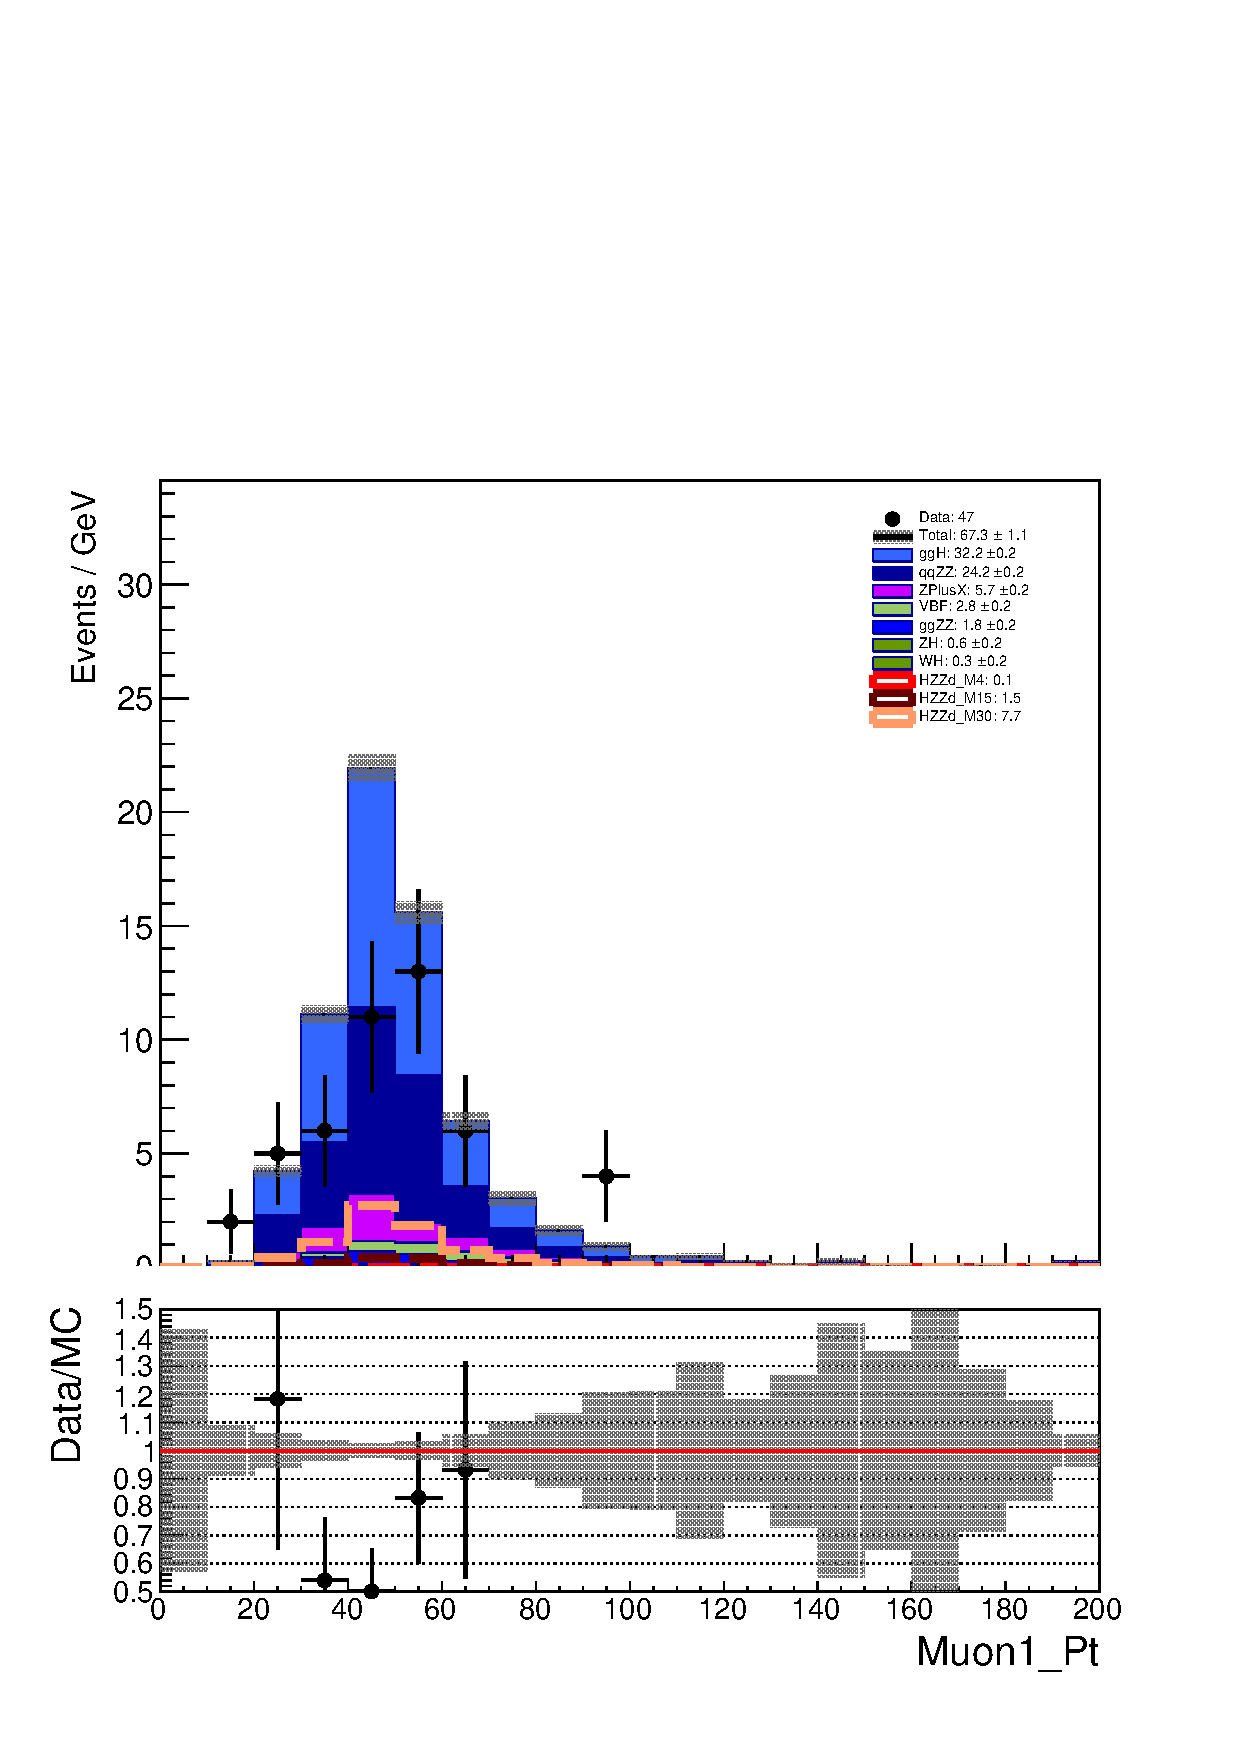
\includegraphics[width=0.49\textwidth]{Figures/Results/Distributions/DarkPhotonSR16/Muon1_Pt}}
{ 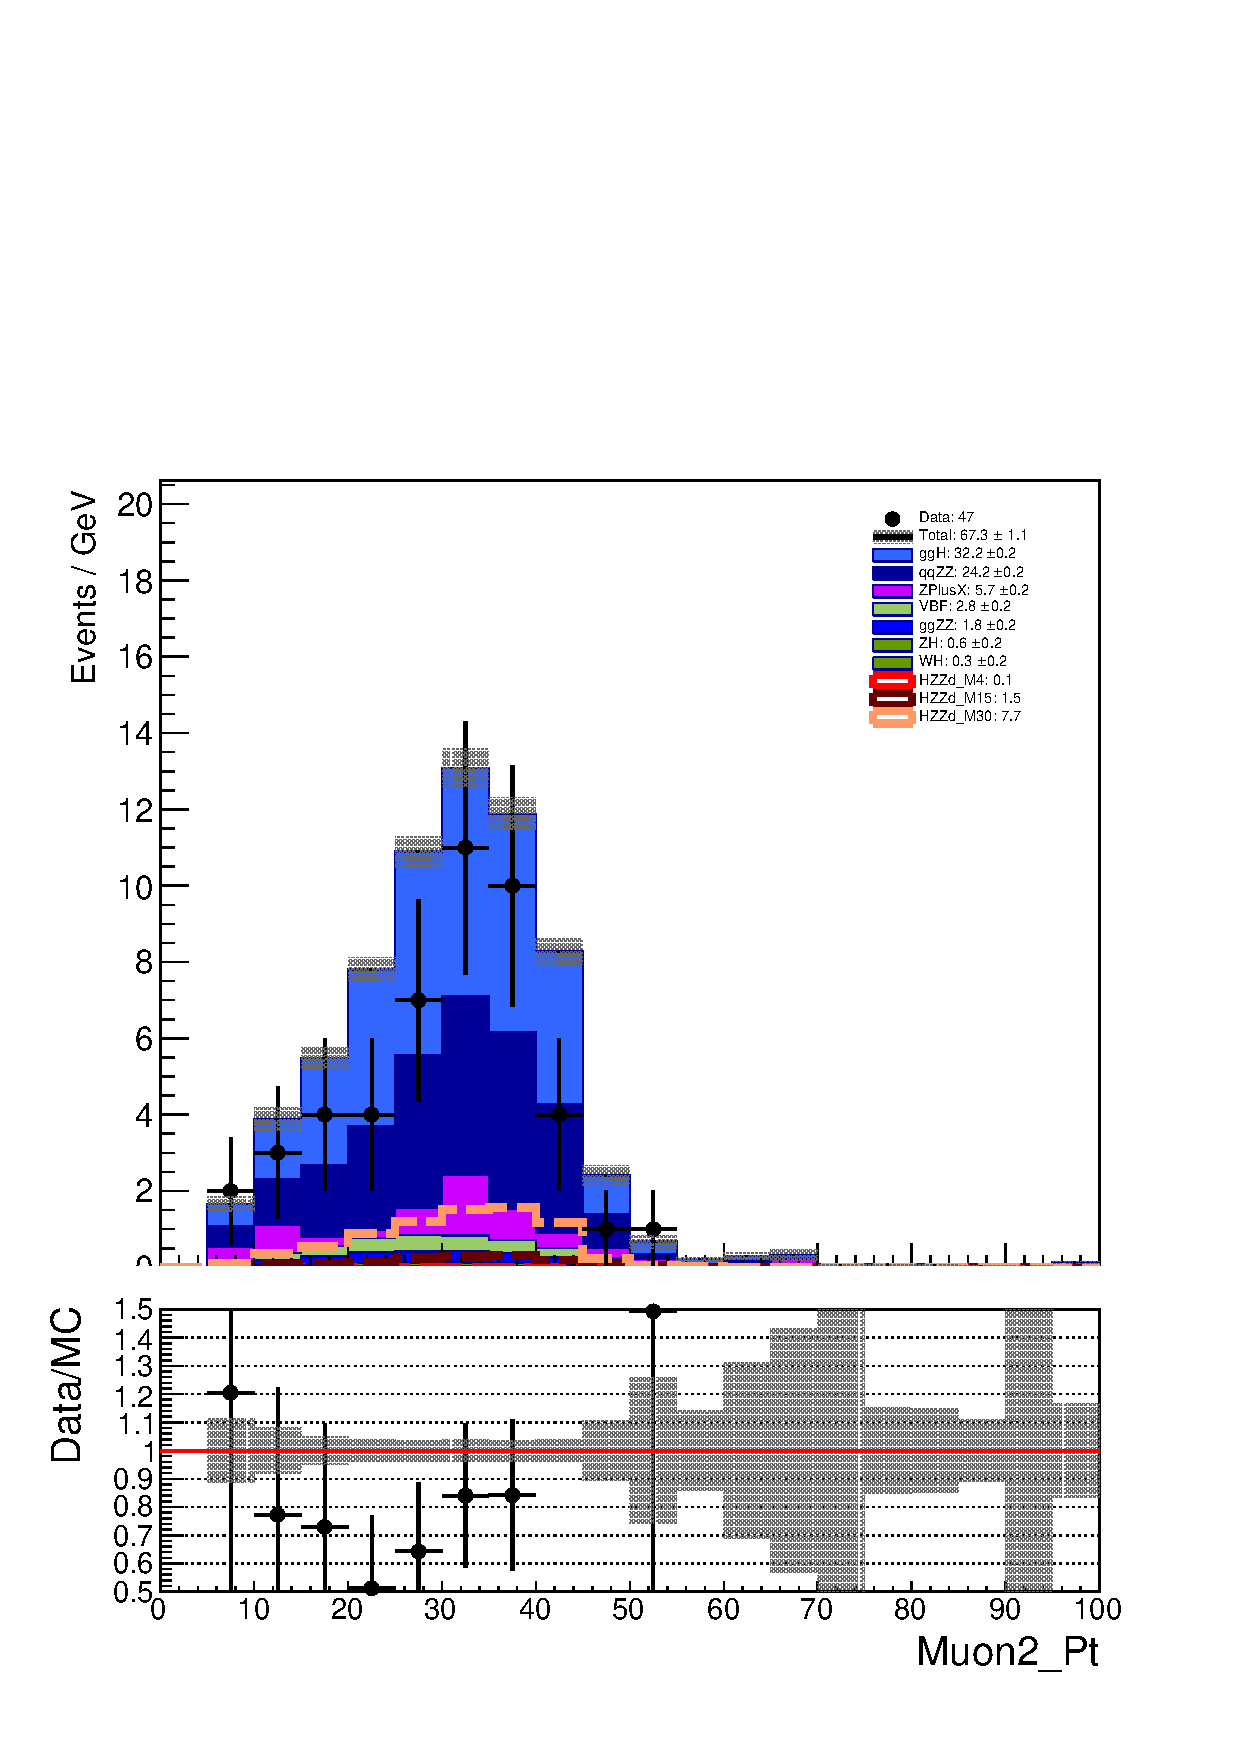
\includegraphics[width=0.49\textwidth]{Figures/Results/Distributions/DarkPhotonSR16/Muon2_Pt}}
{ 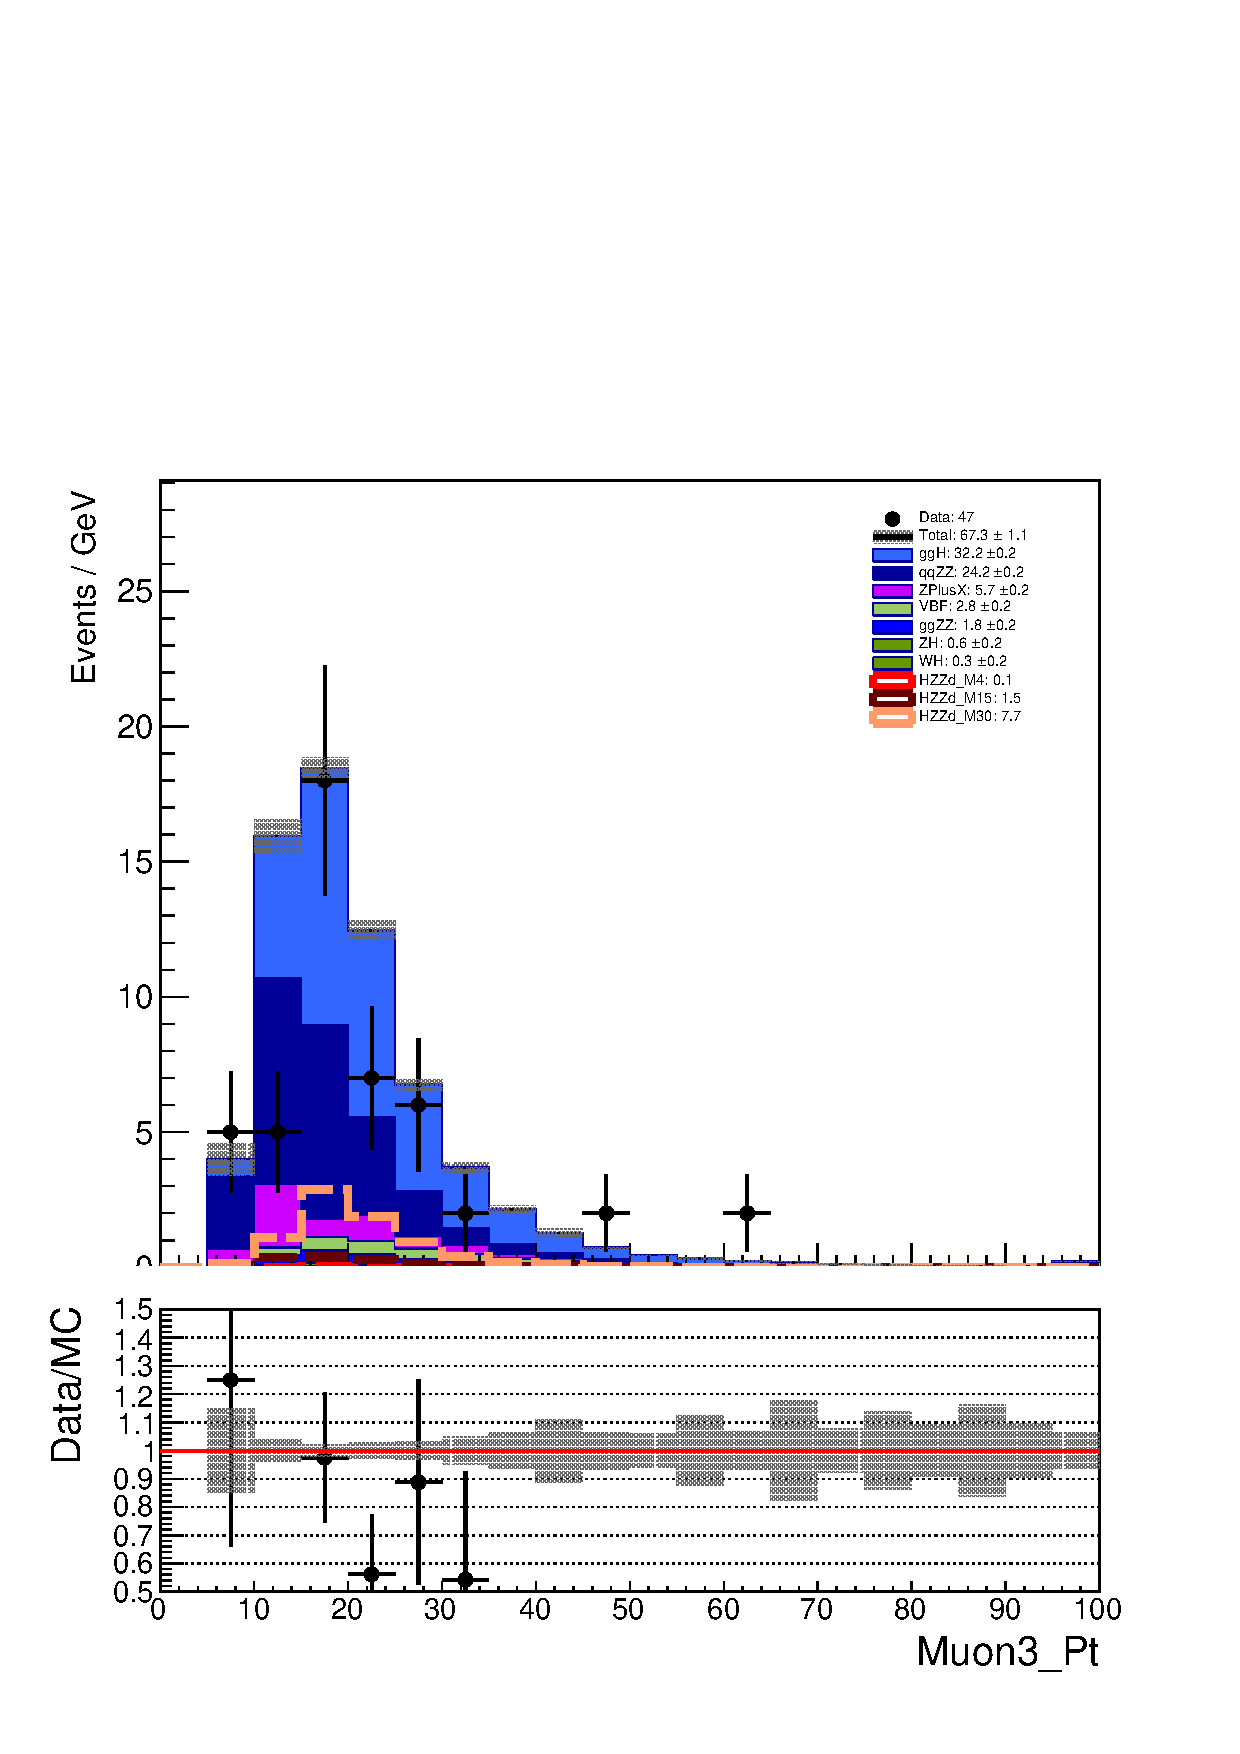
\includegraphics[width=0.49\textwidth]{Figures/Results/Distributions/DarkPhotonSR16/Muon3_Pt}}
{ 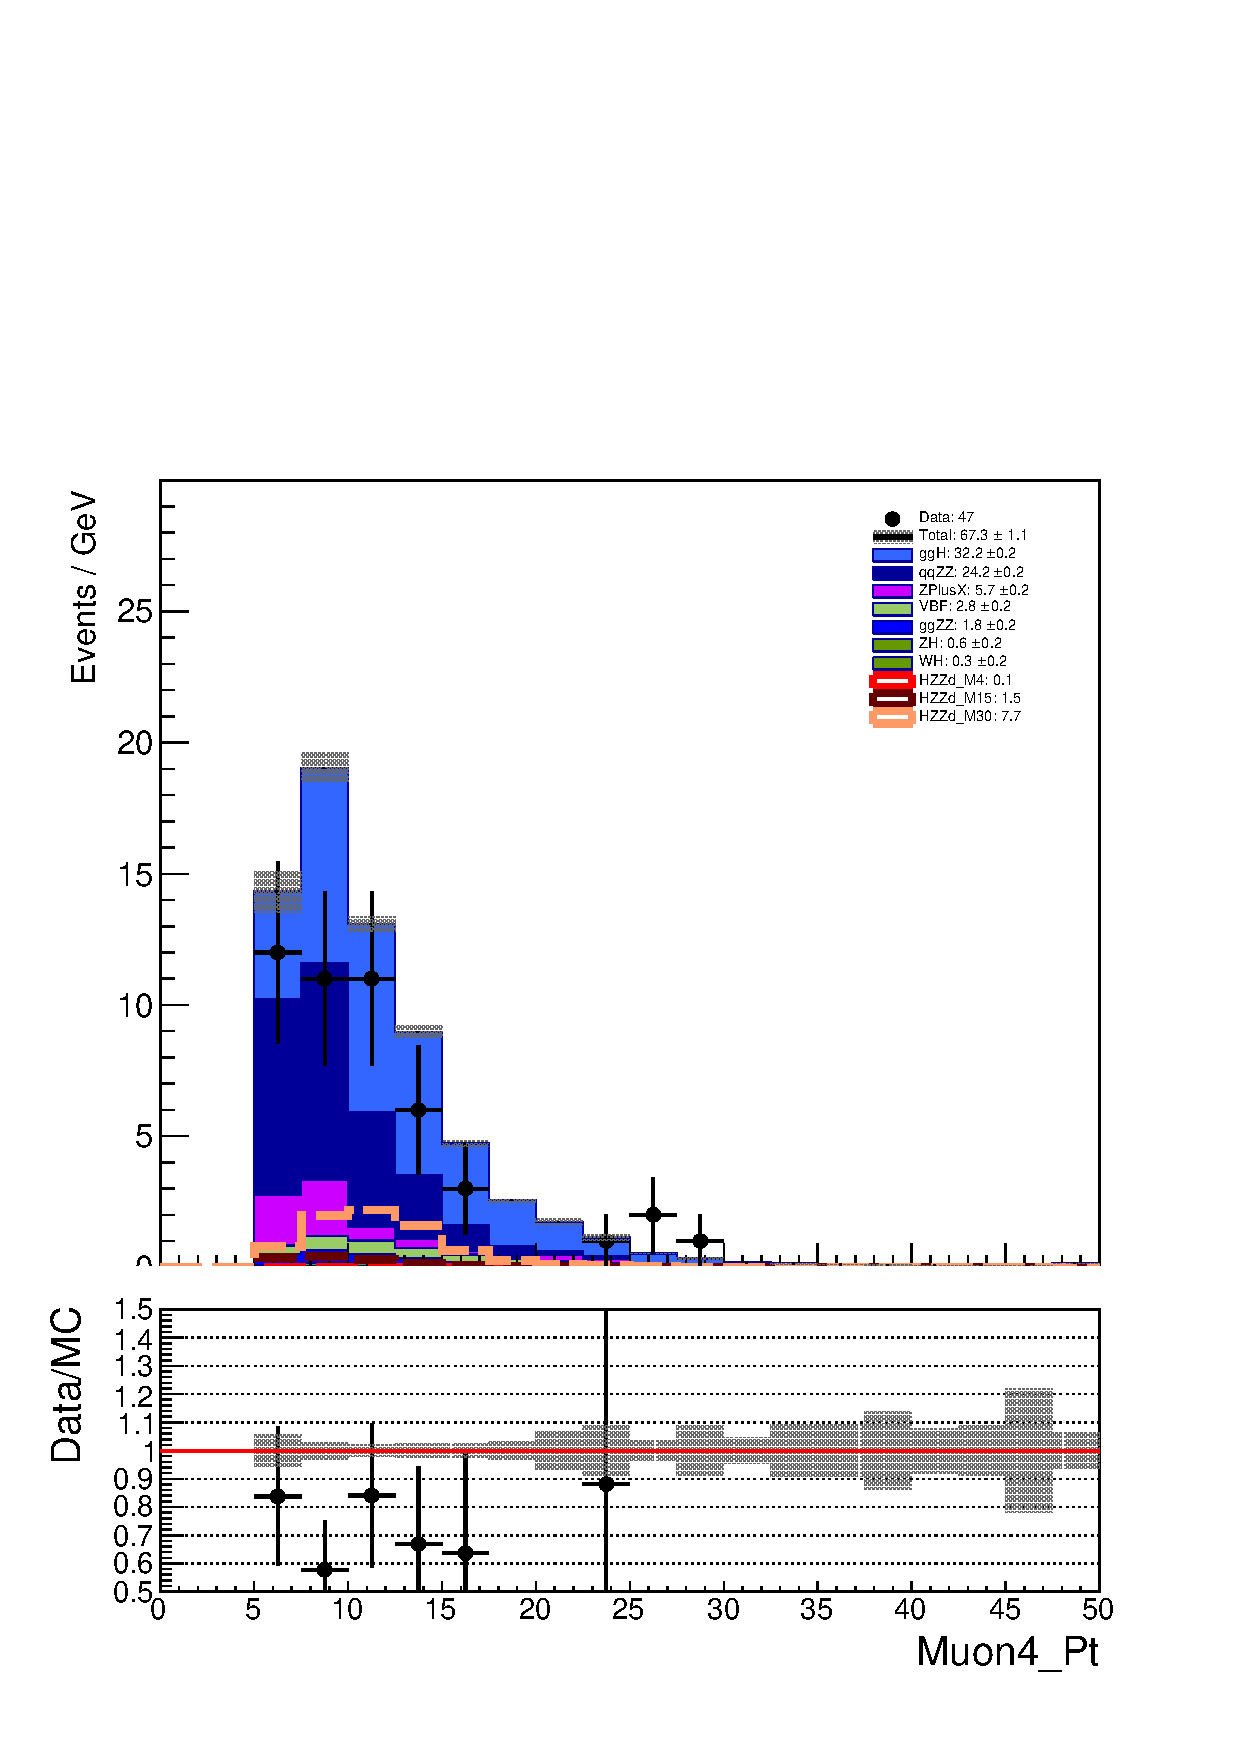
\includegraphics[width=0.49\textwidth]{Figures/Results/Distributions/DarkPhotonSR16/Muon4_Pt}}
\caption{ Distribution of the reconstructed muon~$\pt$ distribution and a comparison to predicted backgrounds using 2016 dataset.
\label{fig:muonPt_16}}
\end{figure}

\begin{figure}[!htbp]
\vspace*{0.3cm}
\centering
{ 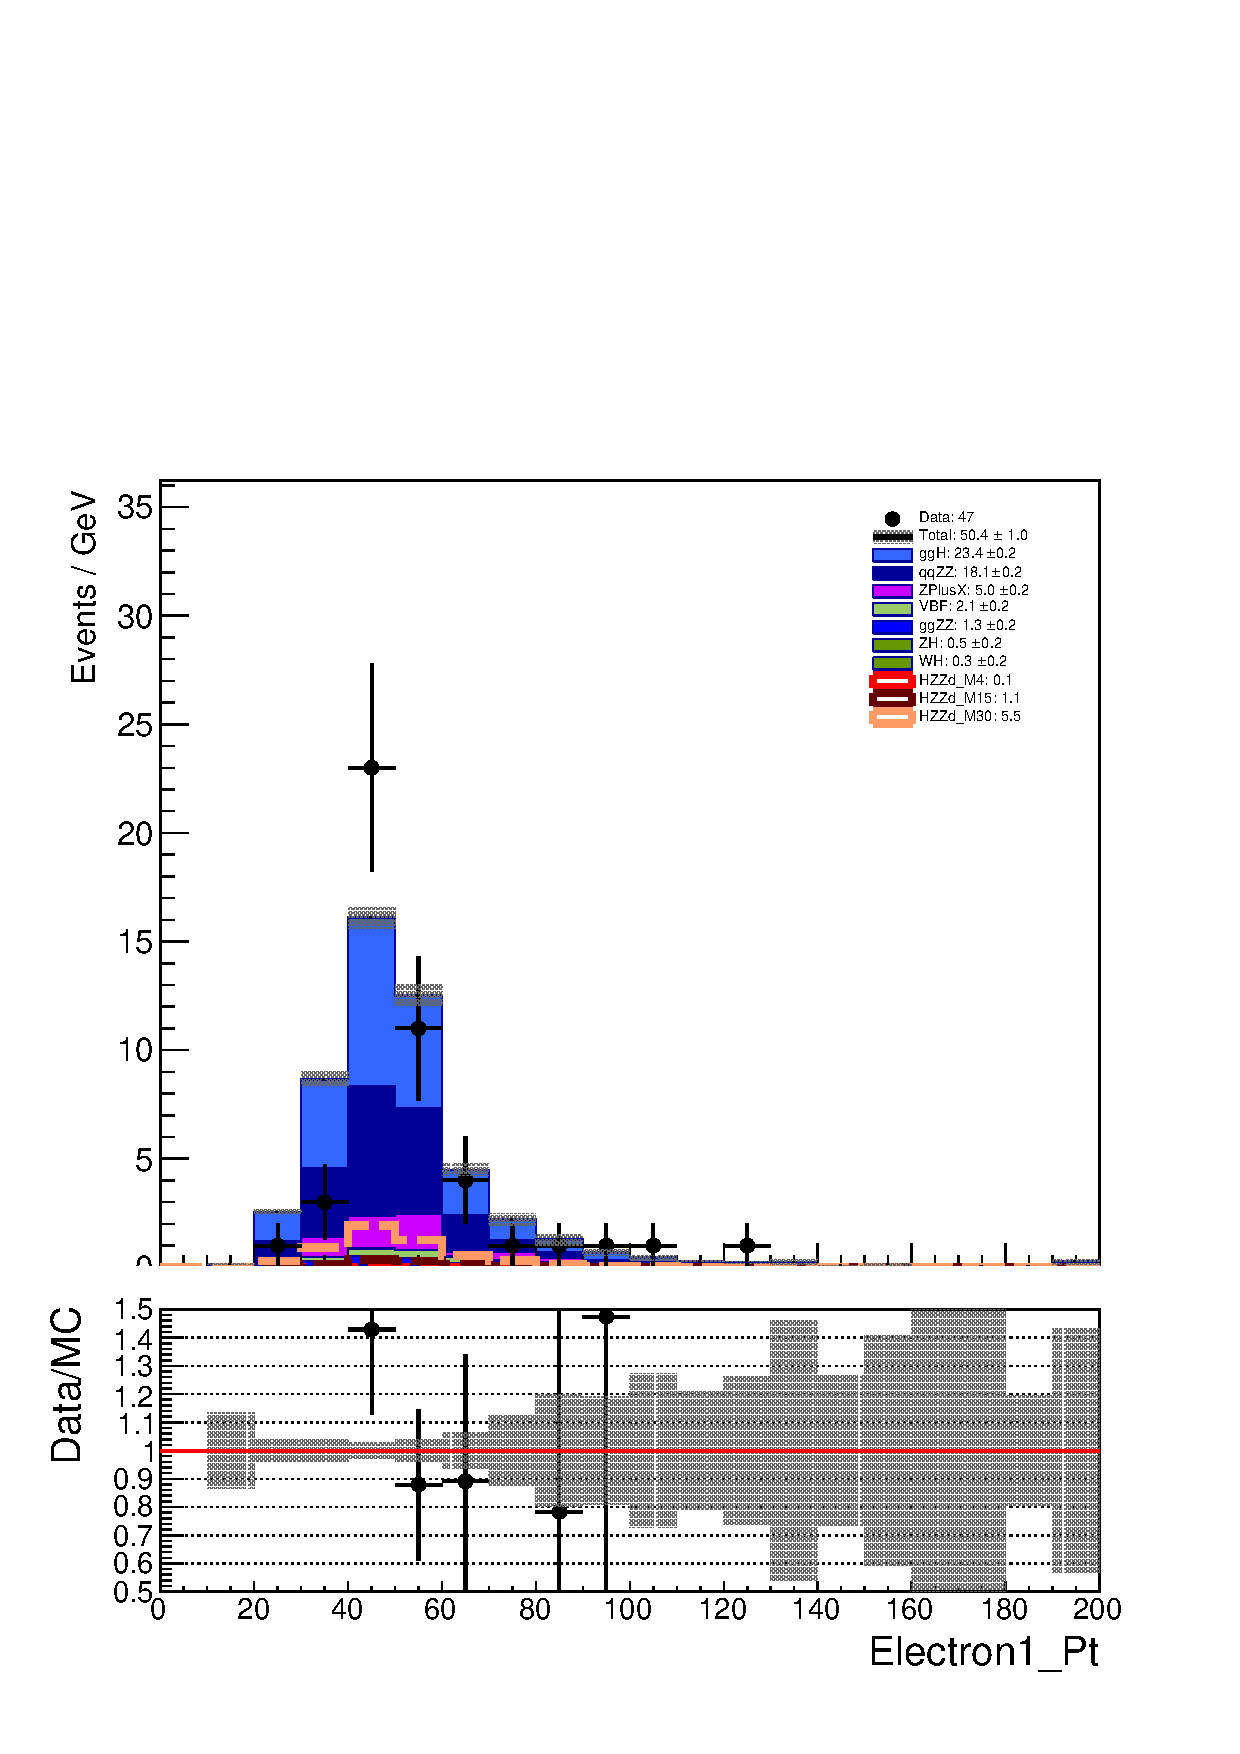
\includegraphics[width=0.49\textwidth]{Figures/Results/Distributions/DarkPhotonSR16/Electron1_Pt}}
{ 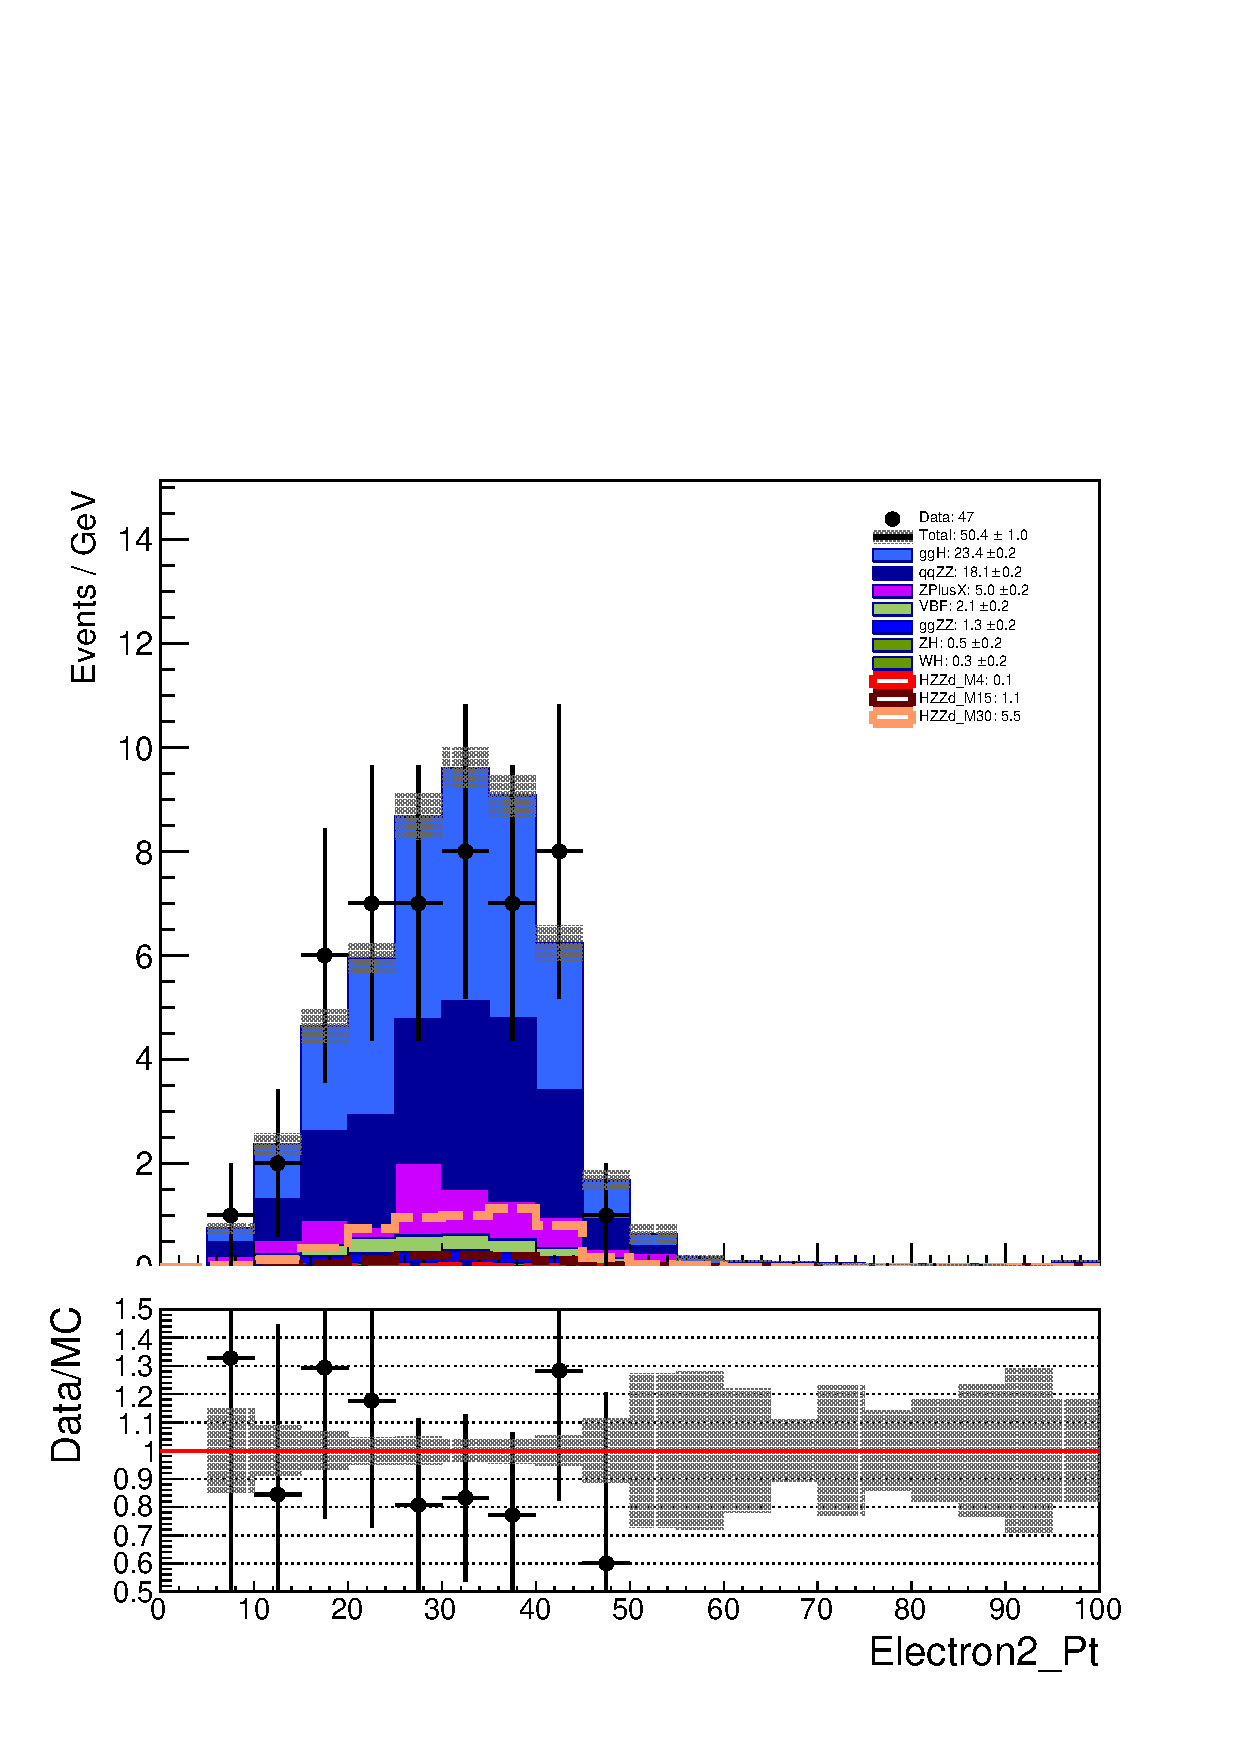
\includegraphics[width=0.49\textwidth]{Figures/Results/Distributions/DarkPhotonSR16/Electron2_Pt}}
{ 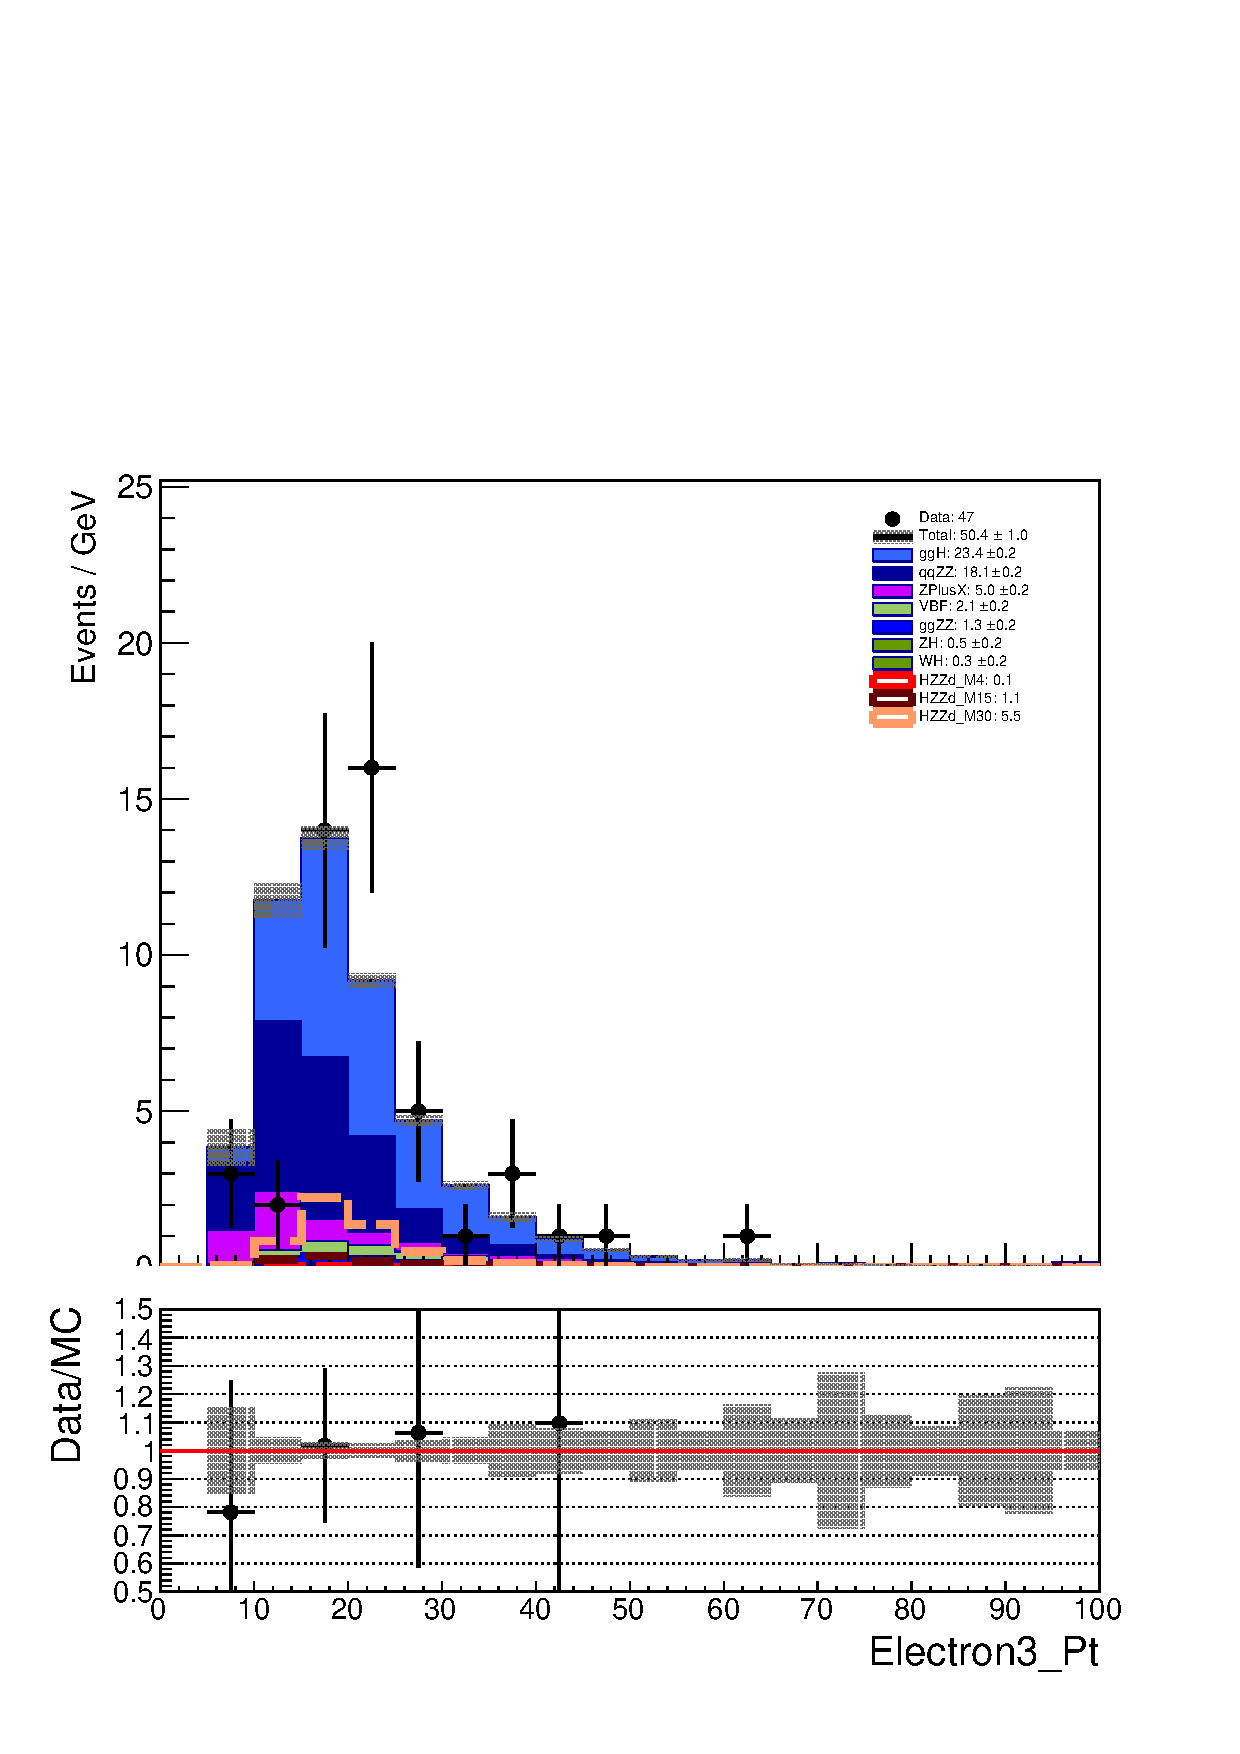
\includegraphics[width=0.49\textwidth]{Figures/Results/Distributions/DarkPhotonSR16/Electron3_Pt}}
{ 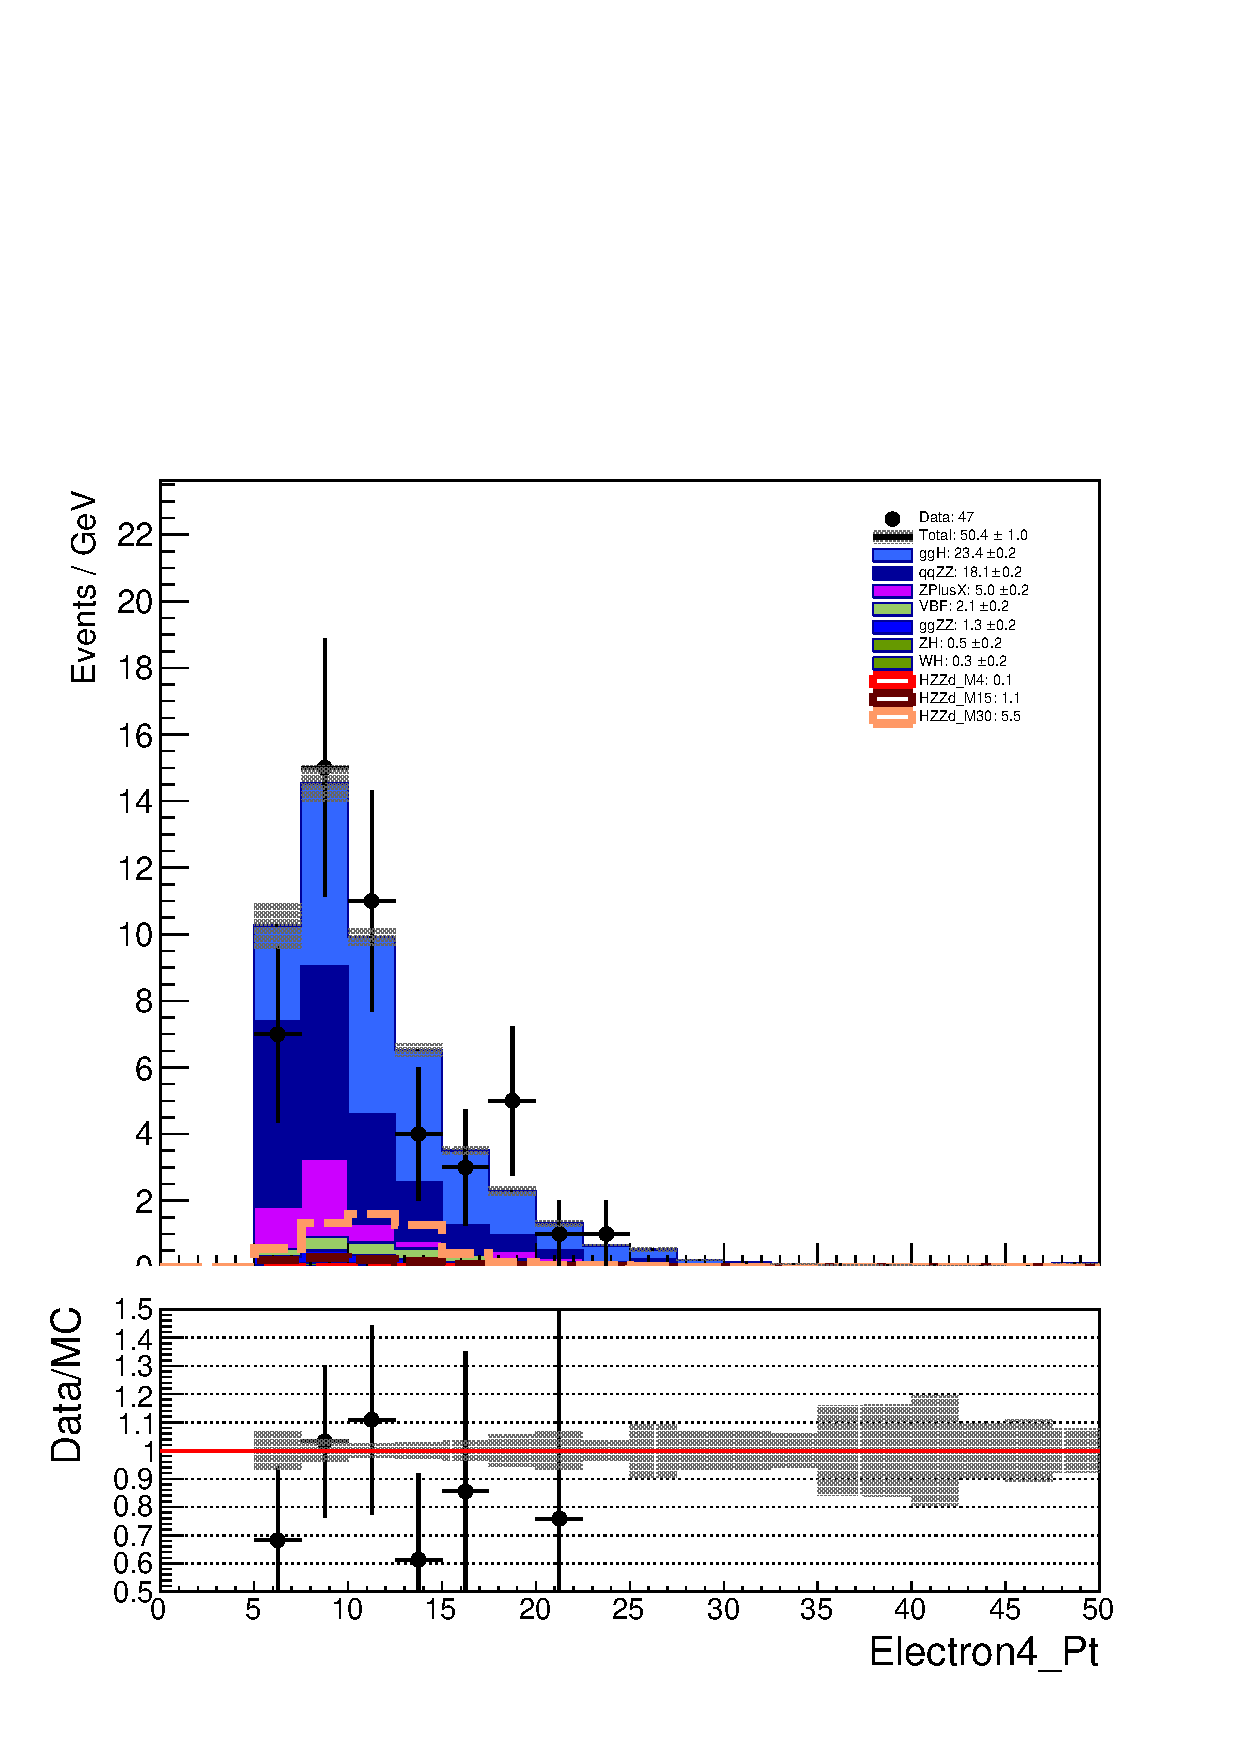
\includegraphics[width=0.49\textwidth]{Figures/Results/Distributions/DarkPhotonSR16/Electron4_Pt}}
\caption{ Distribution of the reconstructed electron~$\pt$ distribution and a comparison to predicted backgrounds using 2016 dataset.
\label{fig:elePt_16}}
\end{figure}

\begin{figure}[!htbp]
\vspace*{0.3cm}
\centering
{ 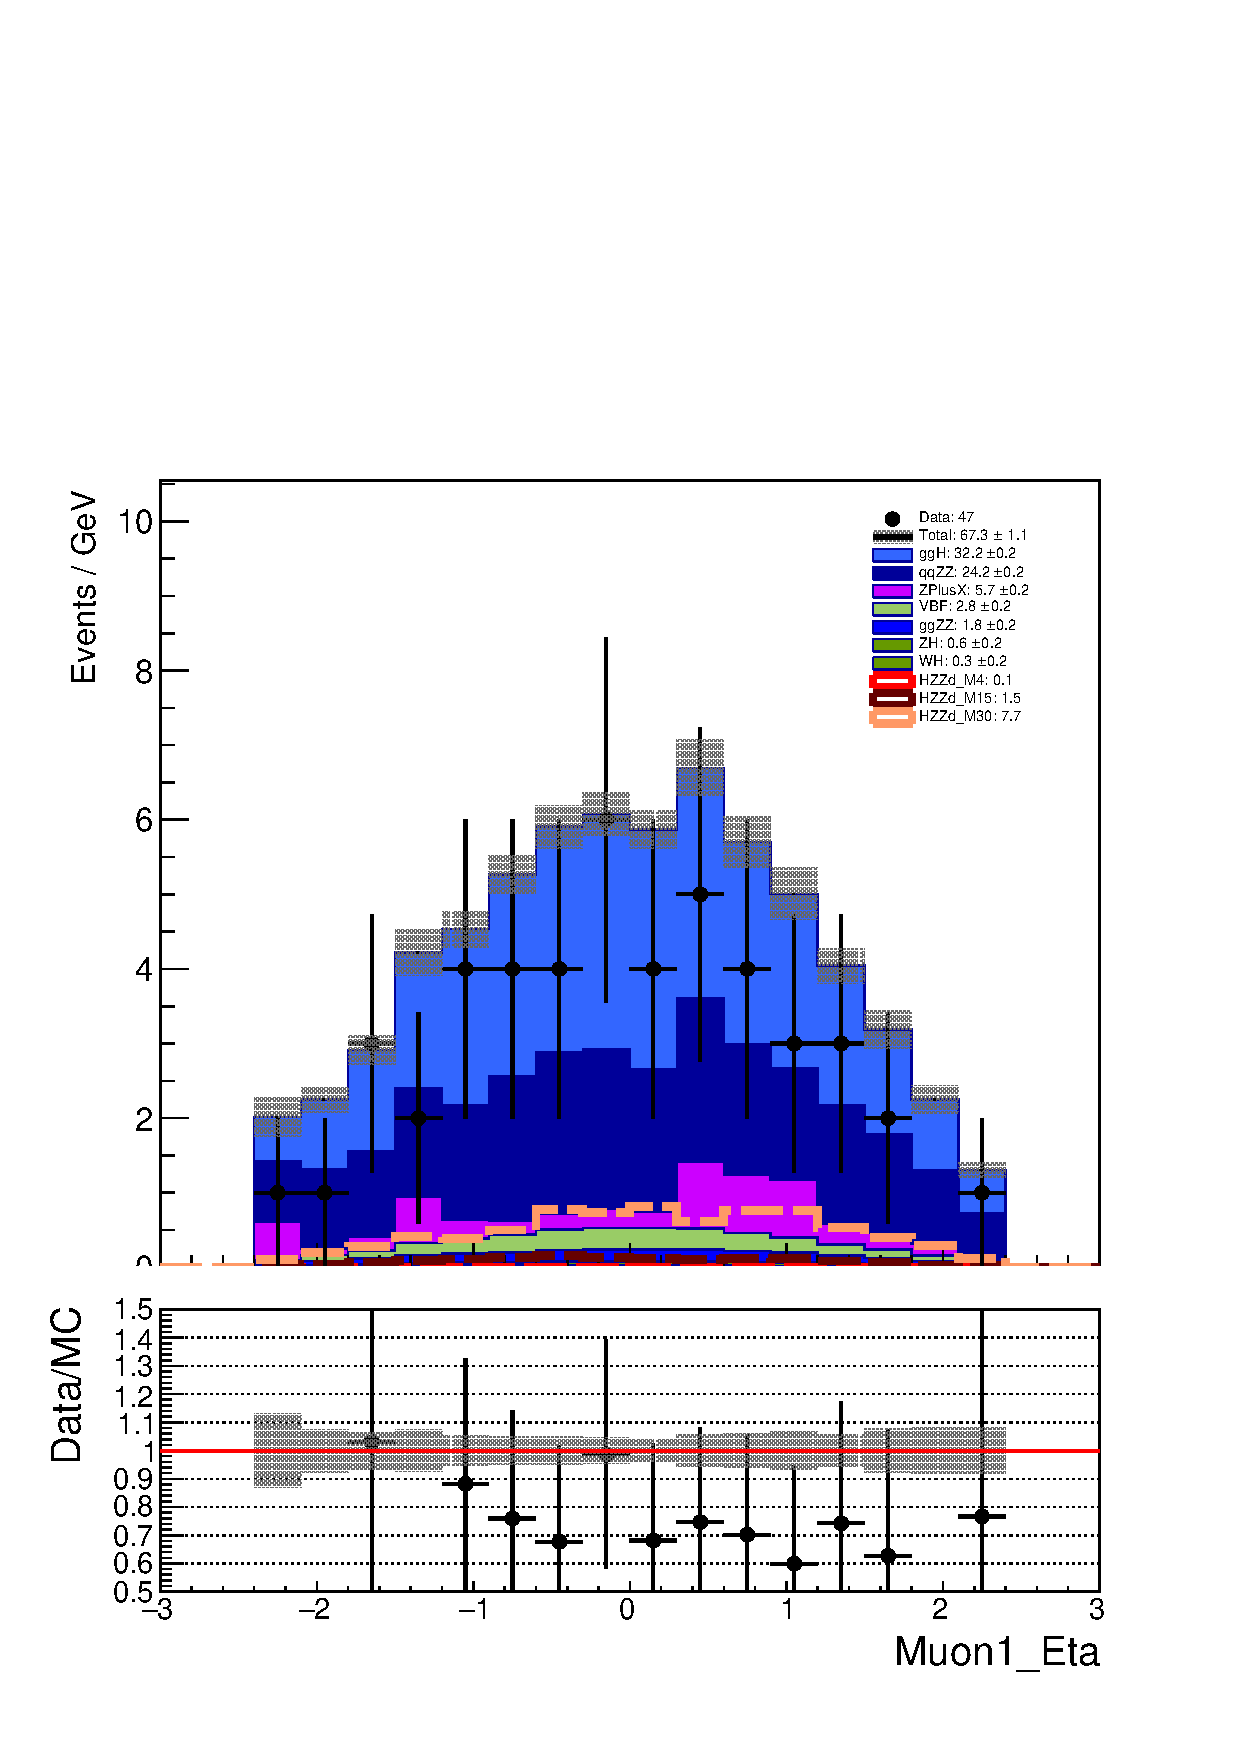
\includegraphics[width=0.49\textwidth]{Figures/Results/Distributions/DarkPhotonSR16/Muon1_Eta}}
{ 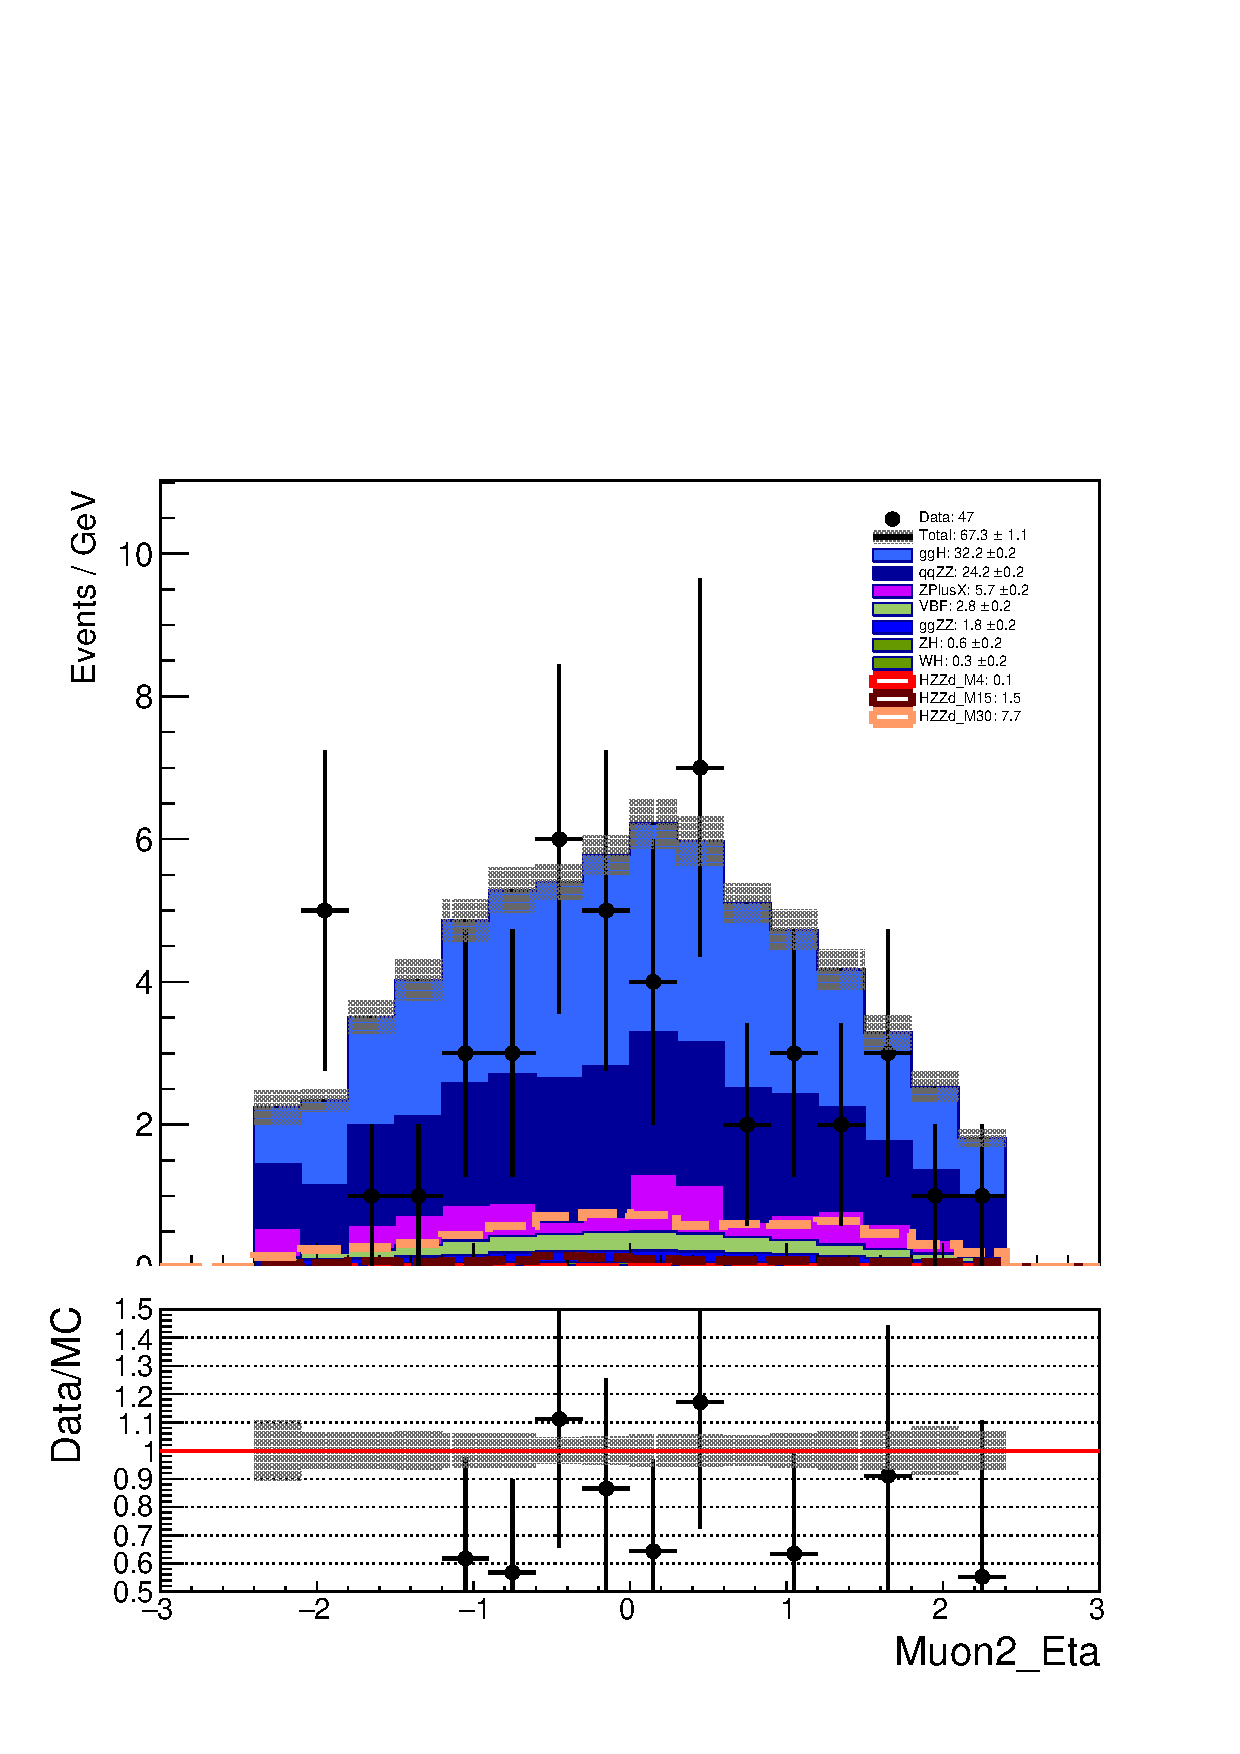
\includegraphics[width=0.49\textwidth]{Figures/Results/Distributions/DarkPhotonSR16/Muon2_Eta}}
{ 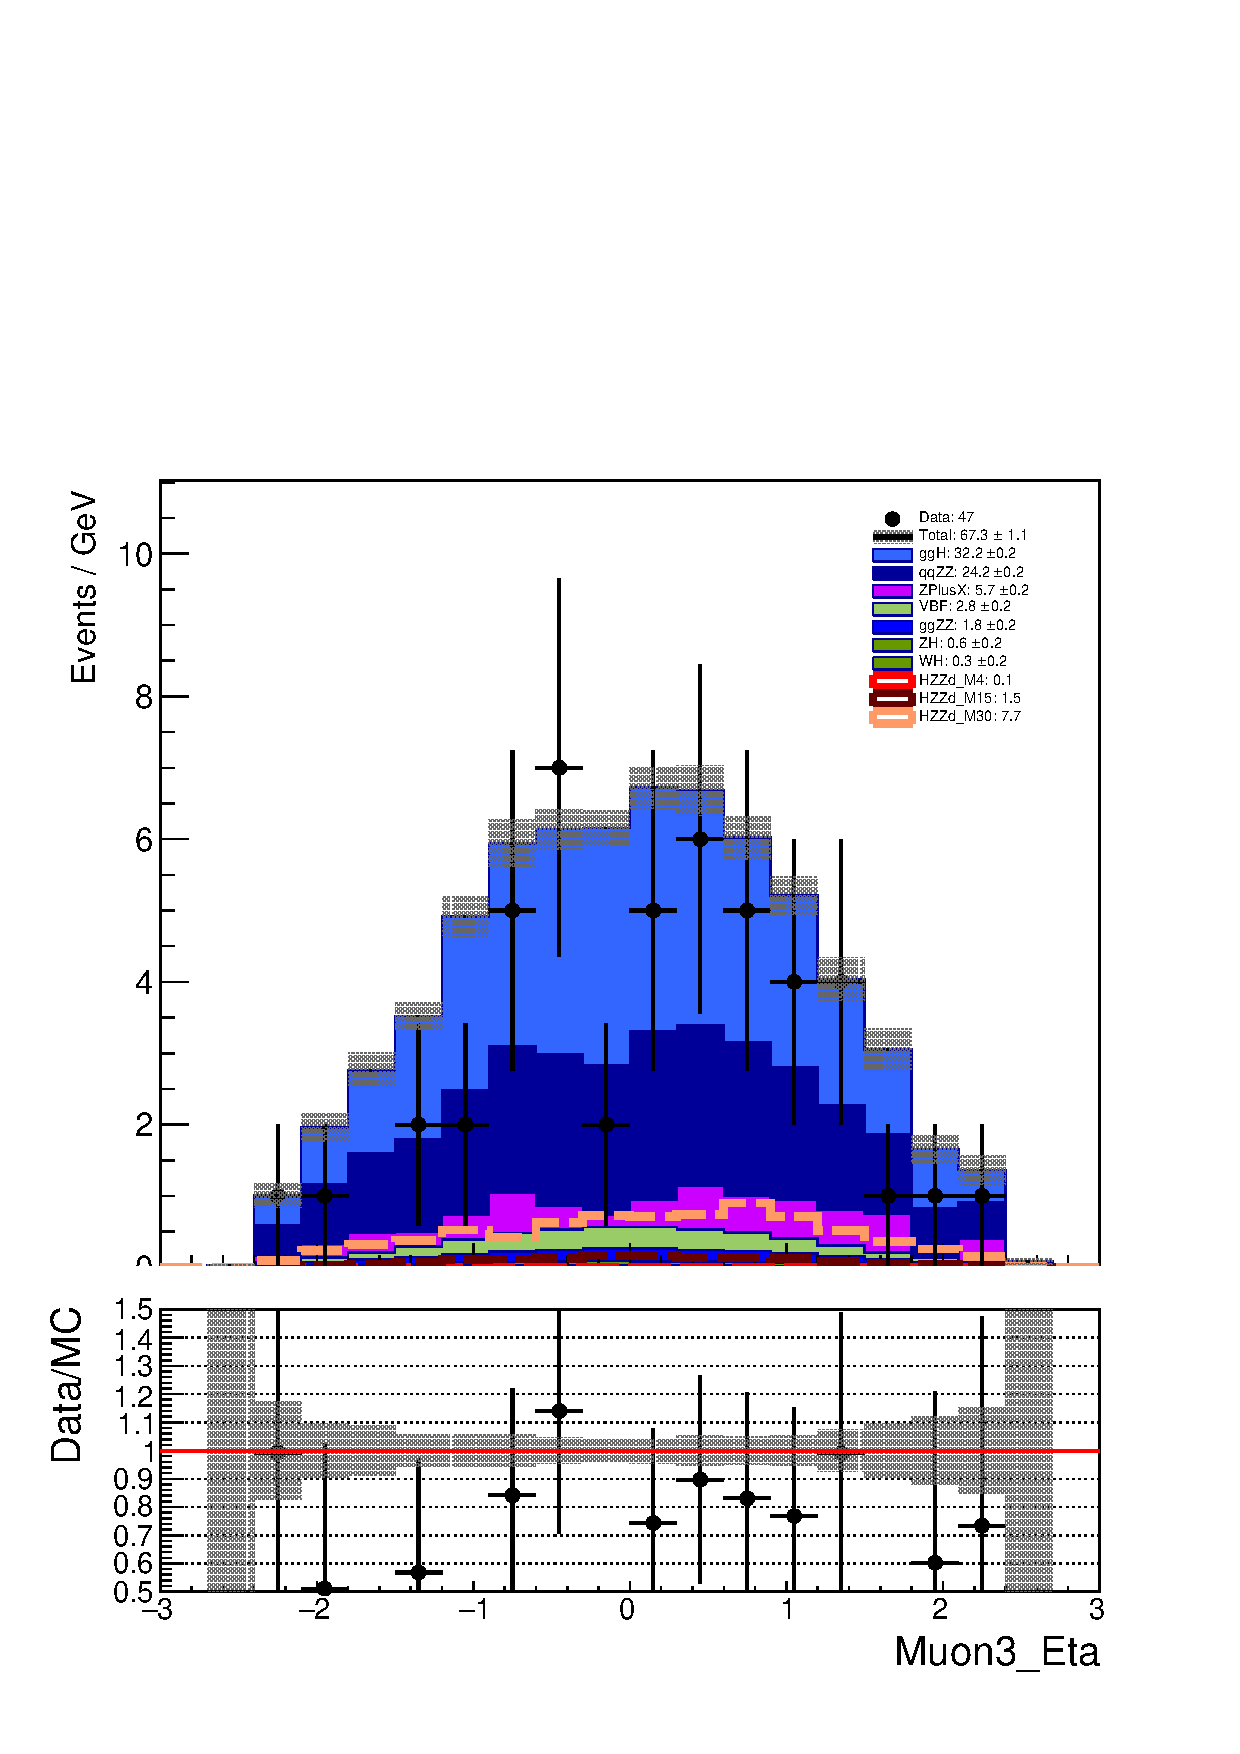
\includegraphics[width=0.49\textwidth]{Figures/Results/Distributions/DarkPhotonSR16/Muon3_Eta}}
{ 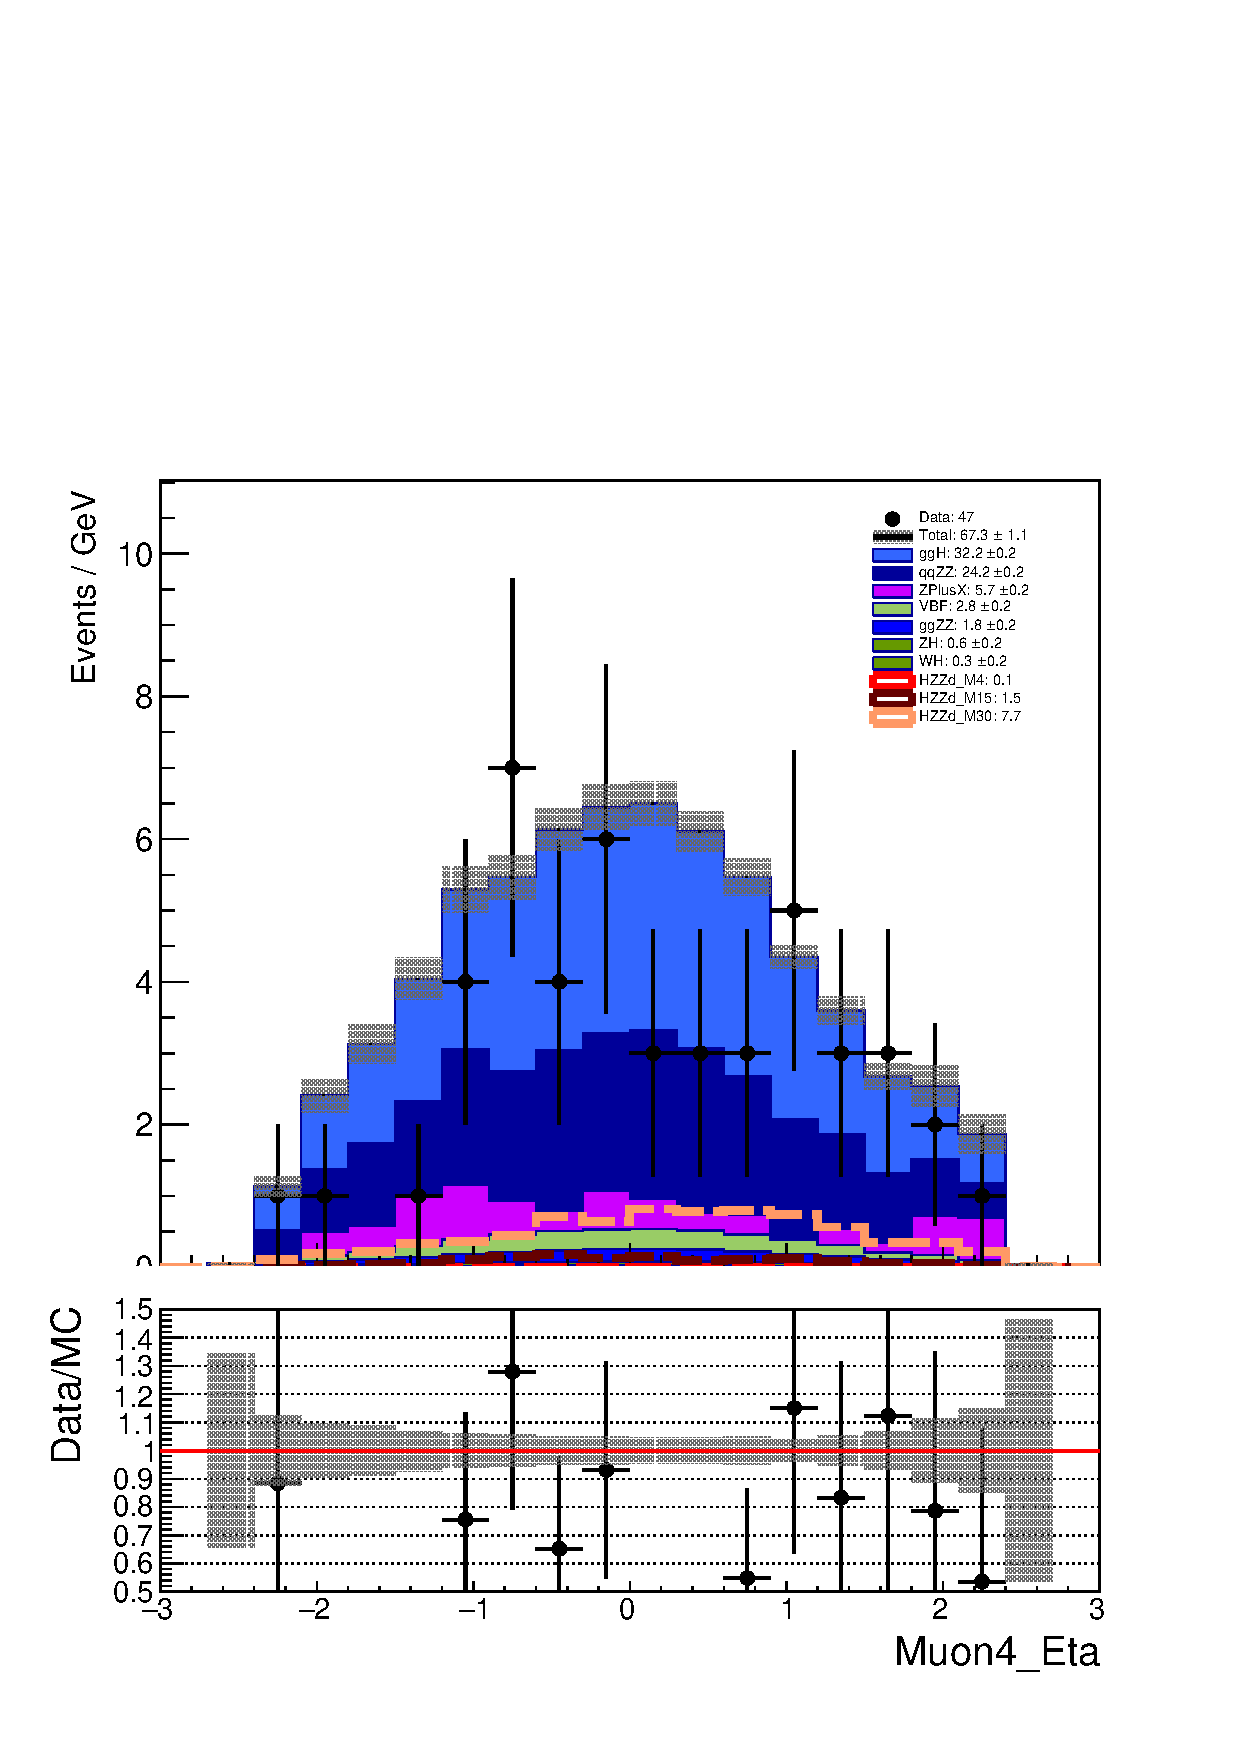
\includegraphics[width=0.49\textwidth]{Figures/Results/Distributions/DarkPhotonSR16/Muon4_Eta}}
\caption{ Distribution of the reconstructed muon~$\eta$ distribution and a comparison to predicted backgrounds using 2016 dataset.
\label{fig:muonEta_16}}
\end{figure}

\begin{figure}[!htbp]
\vspace*{0.3cm}
\centering
{ 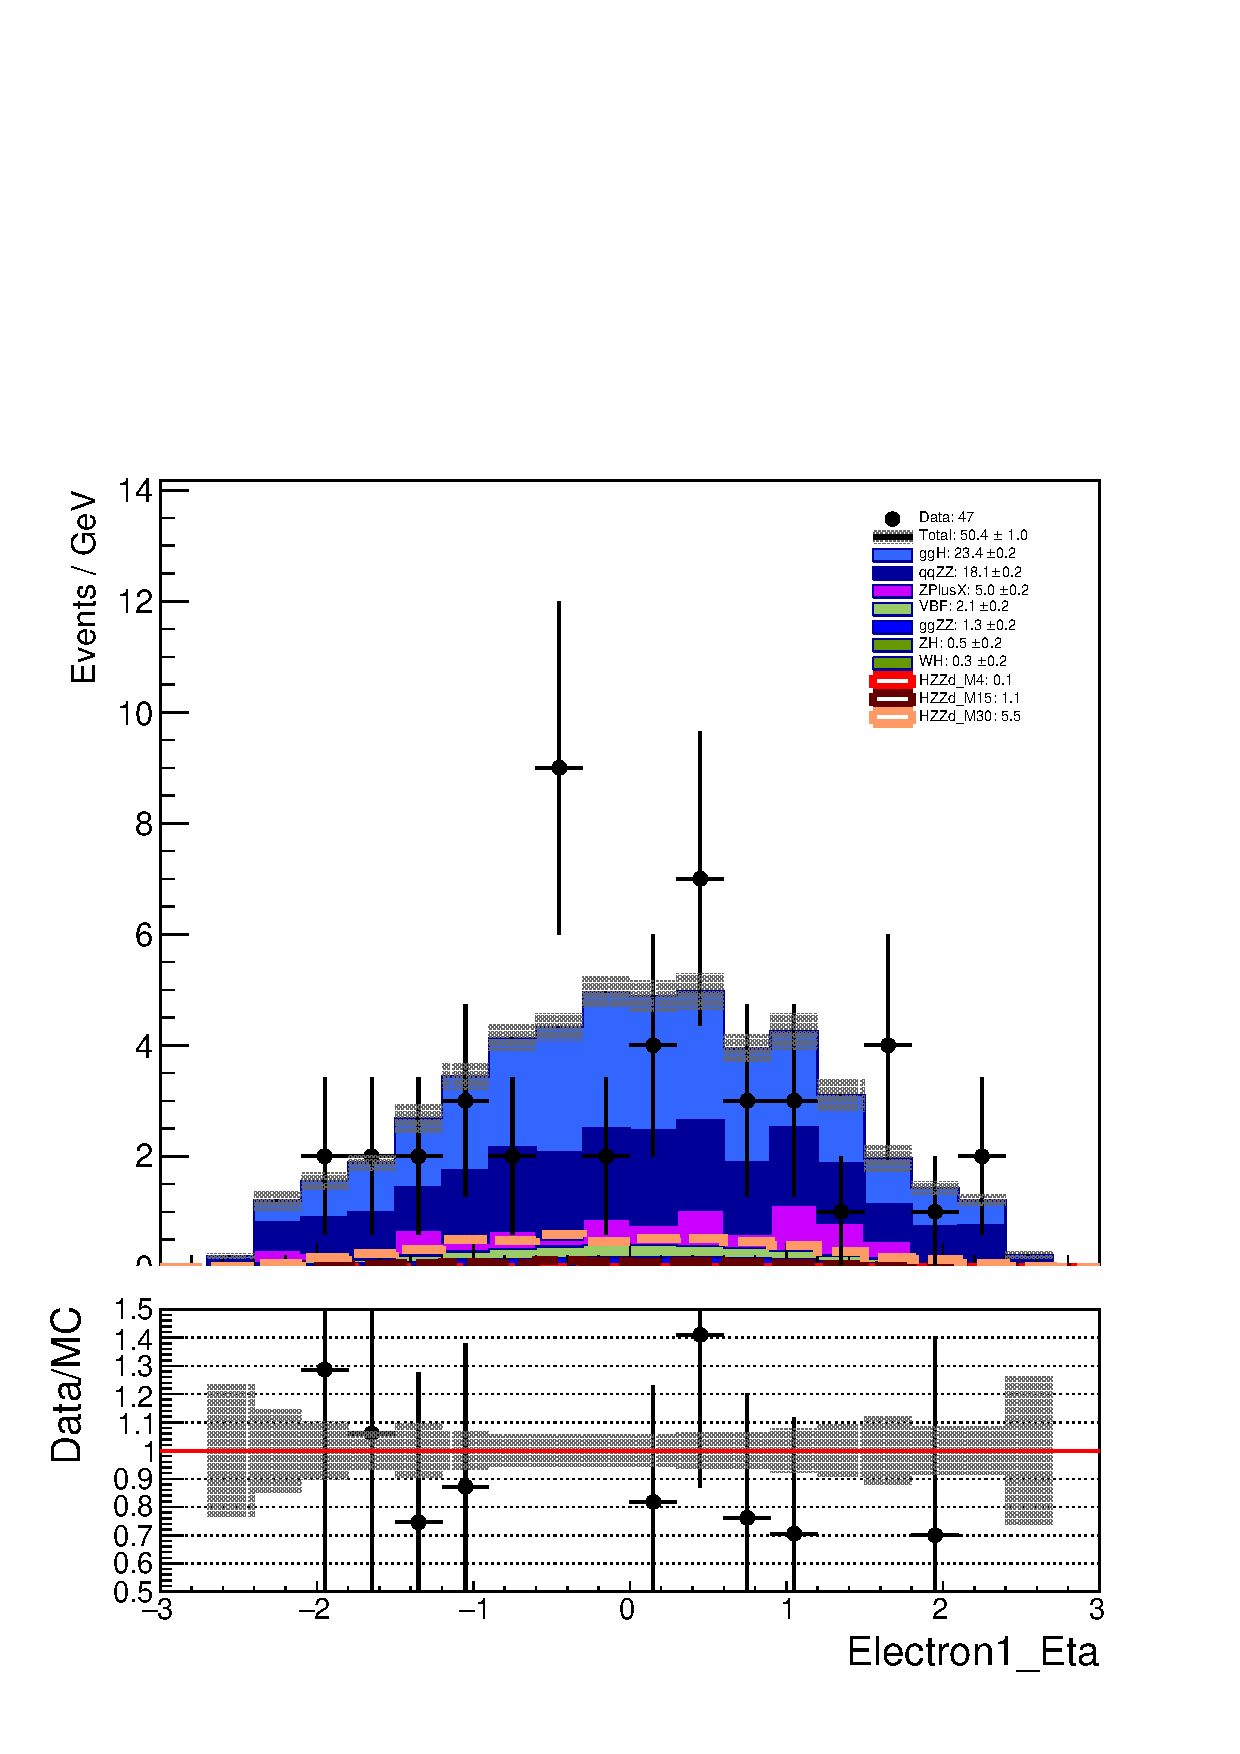
\includegraphics[width=0.49\textwidth]{Figures/Results/Distributions/DarkPhotonSR16/Electron1_Eta}}
{ 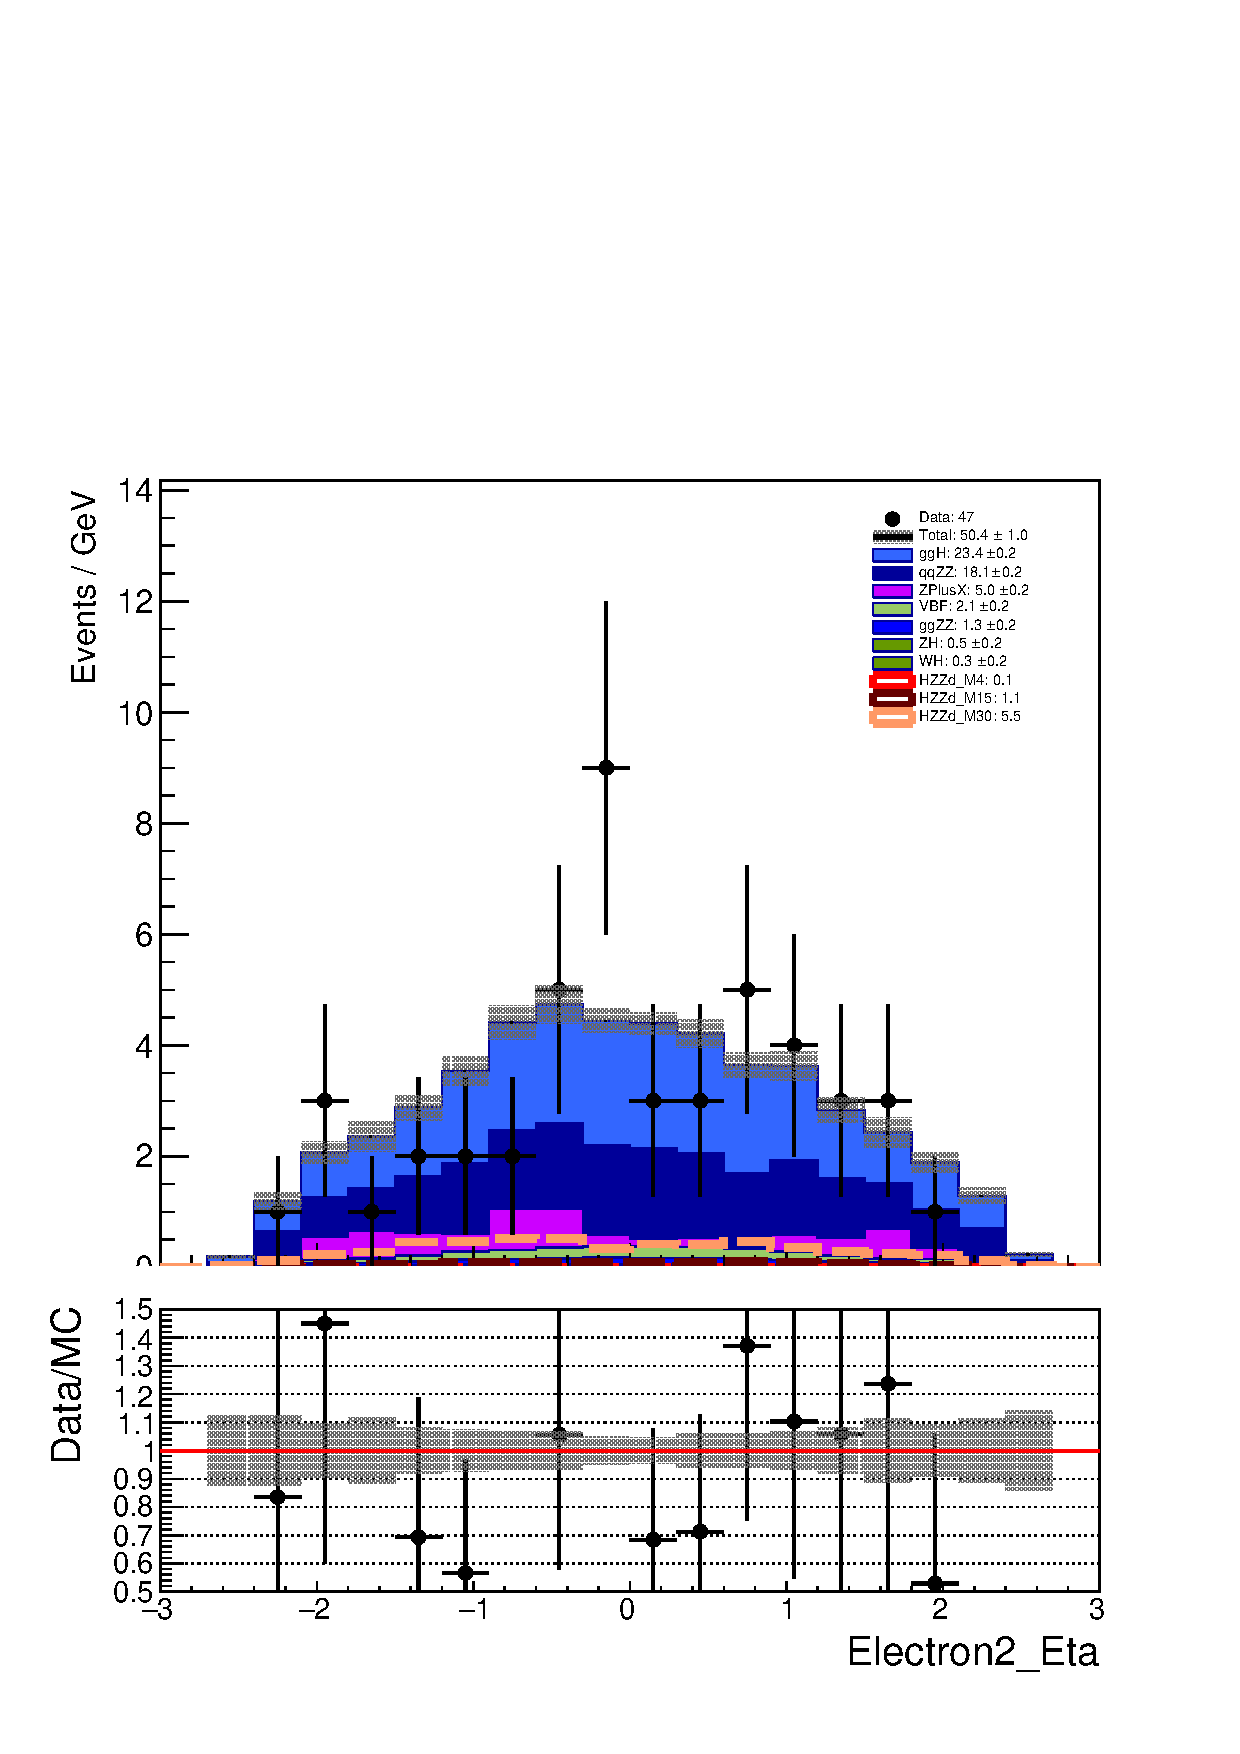
\includegraphics[width=0.49\textwidth]{Figures/Results/Distributions/DarkPhotonSR16/Electron2_Eta}}
{ 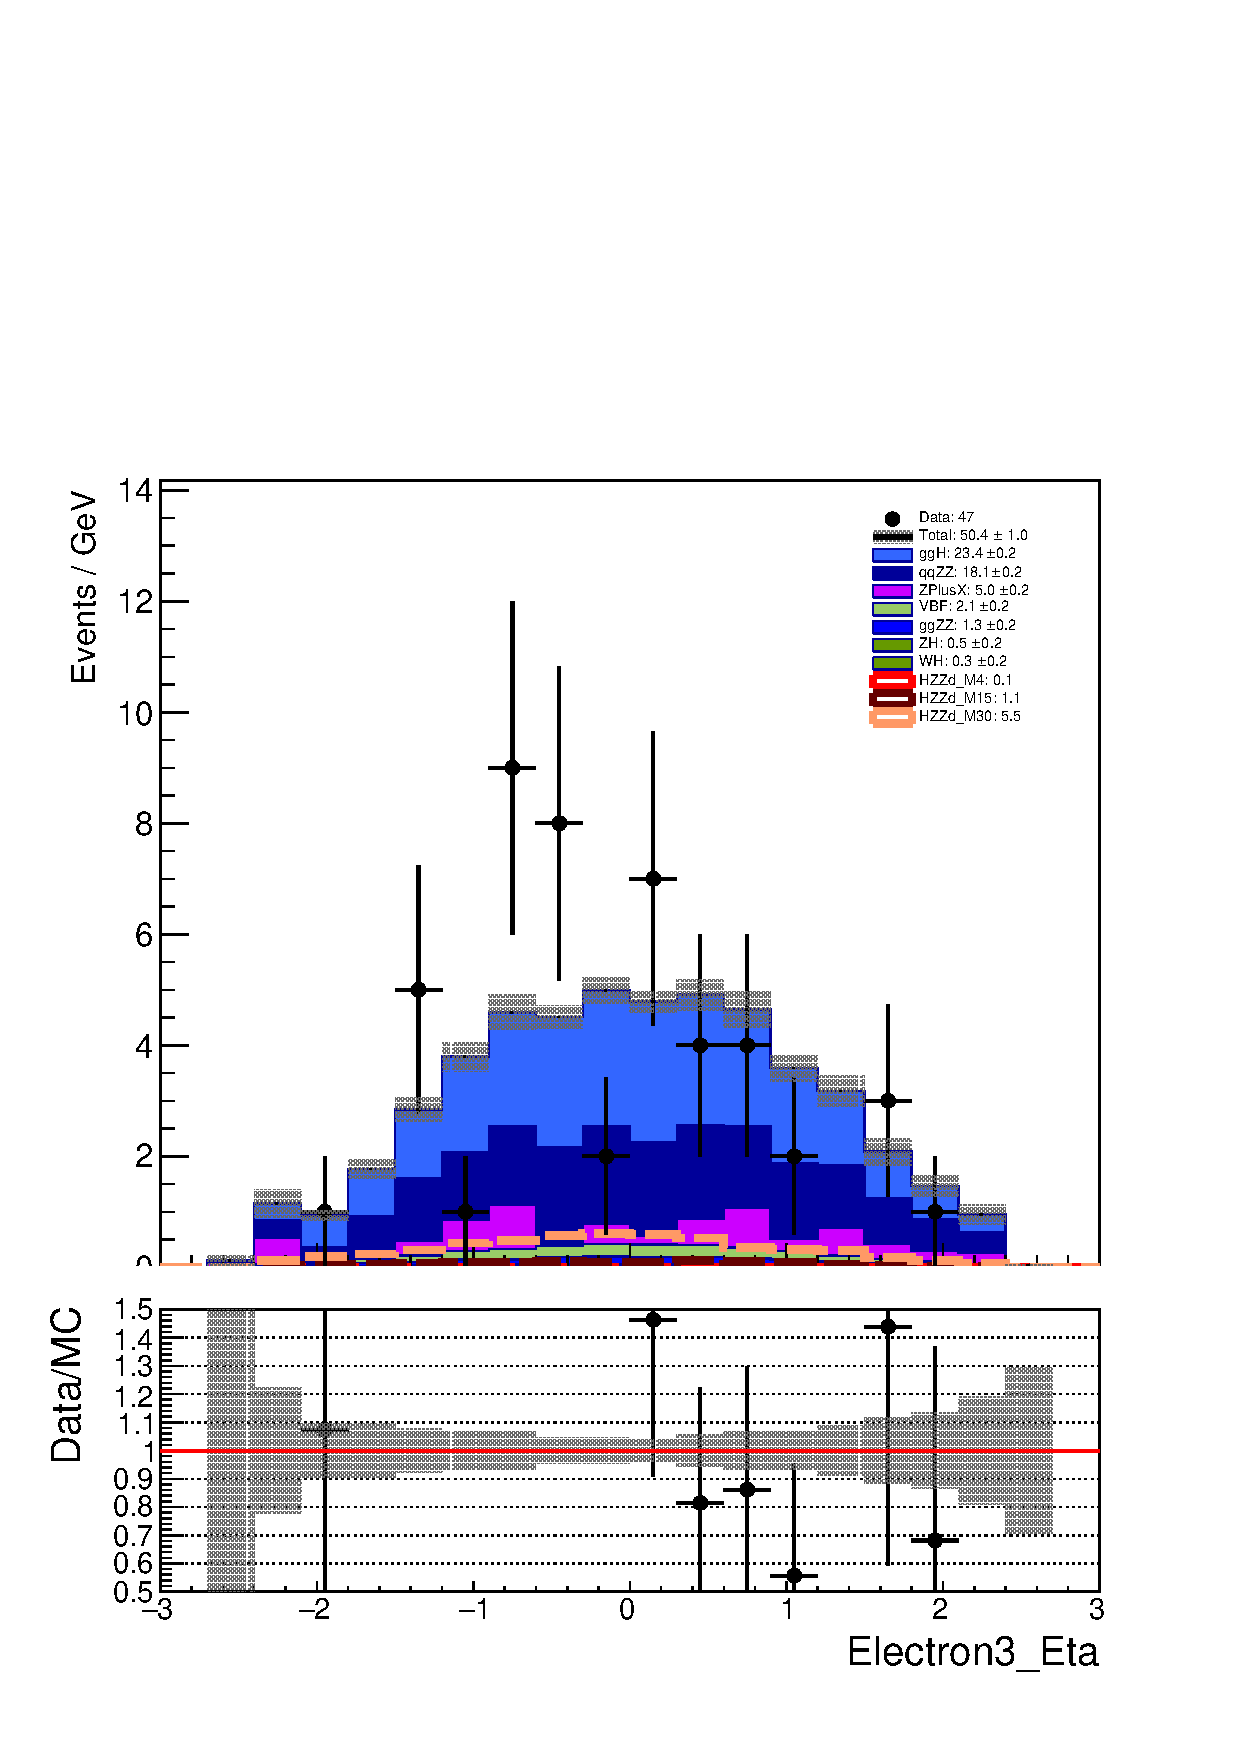
\includegraphics[width=0.49\textwidth]{Figures/Results/Distributions/DarkPhotonSR16/Electron3_Eta}}
{ 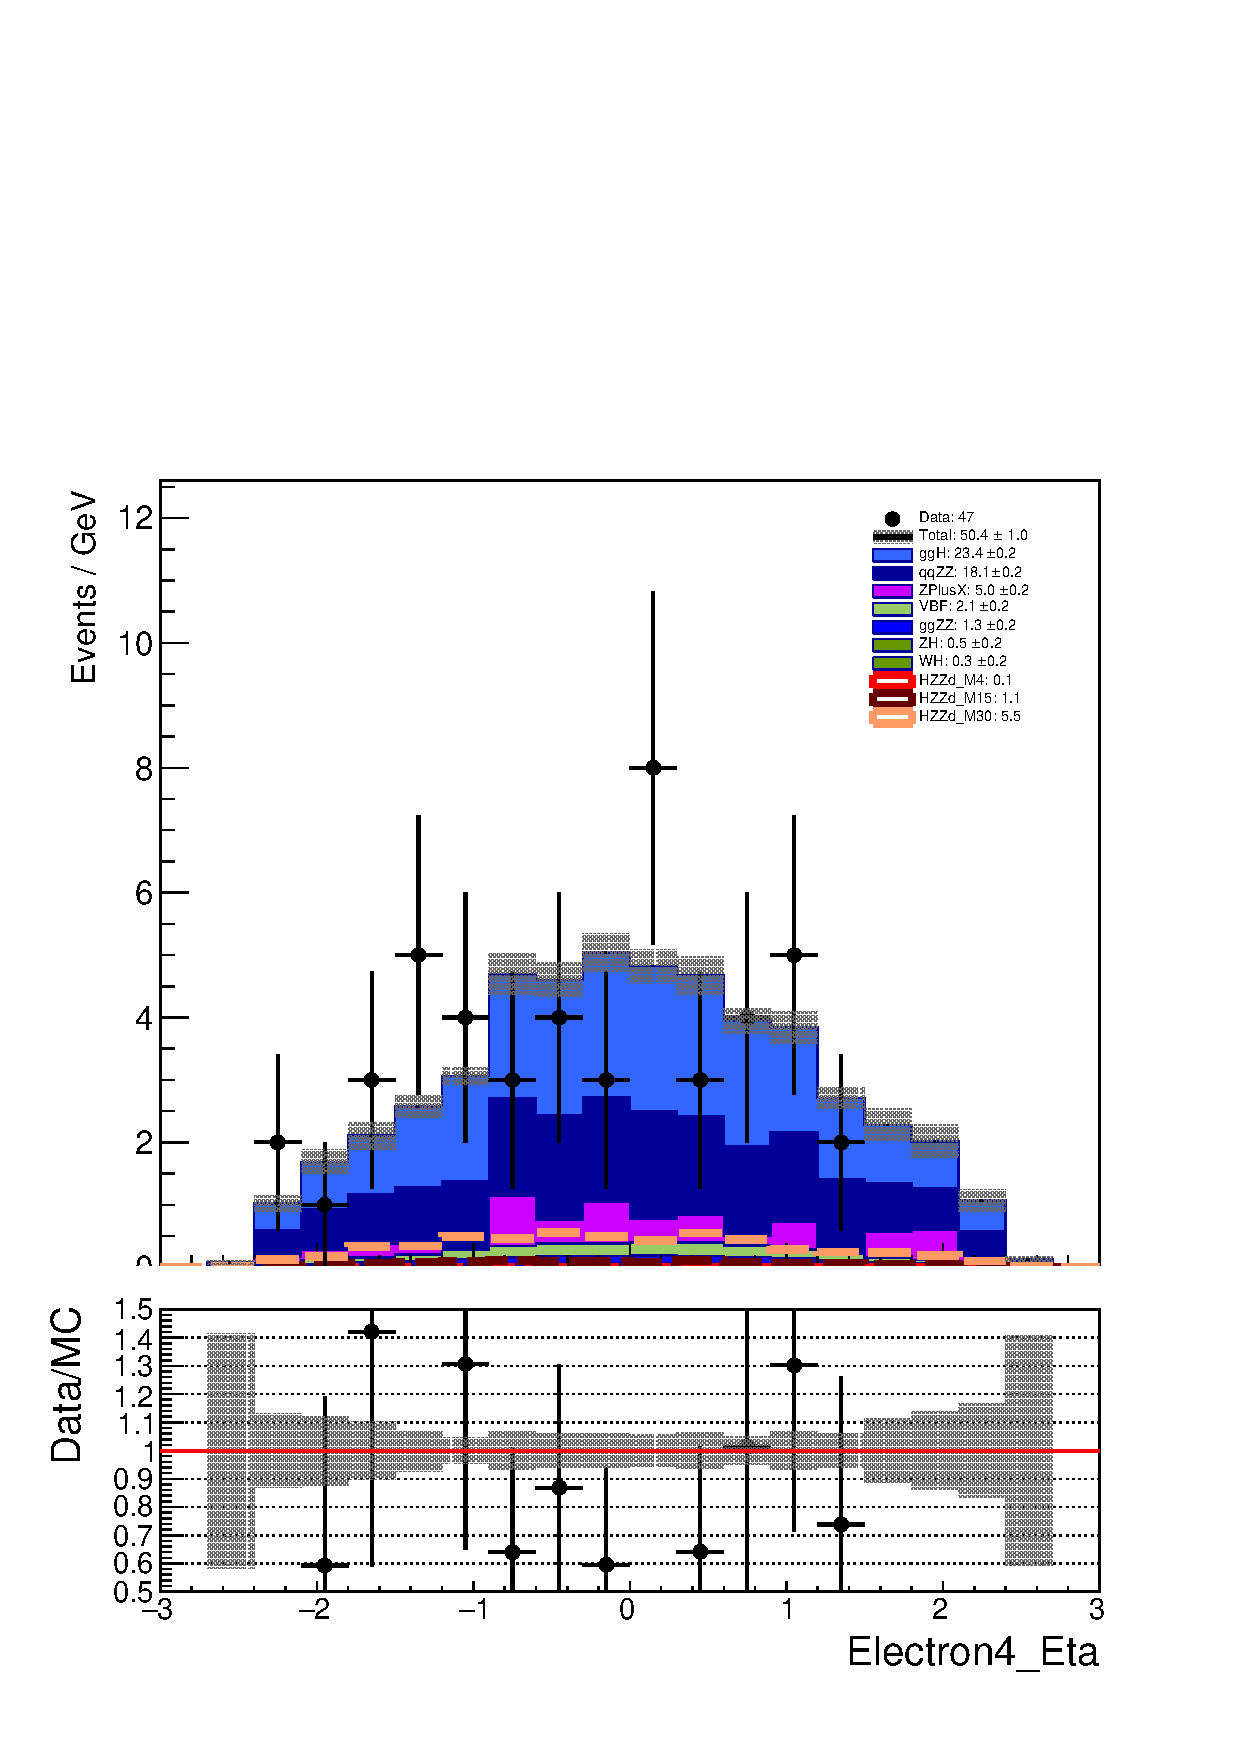
\includegraphics[width=0.49\textwidth]{Figures/Results/Distributions/DarkPhotonSR16/Electron4_Eta}}
\caption{ Distribution of the reconstructed electron~$\eta$ distribution and a comparison to predicted backgrounds using 2016 dataset.
\label{fig:eleEta_16}}
\end{figure}

\begin{figure}[!htbp]
\vspace*{0.3cm}
\centering
{ 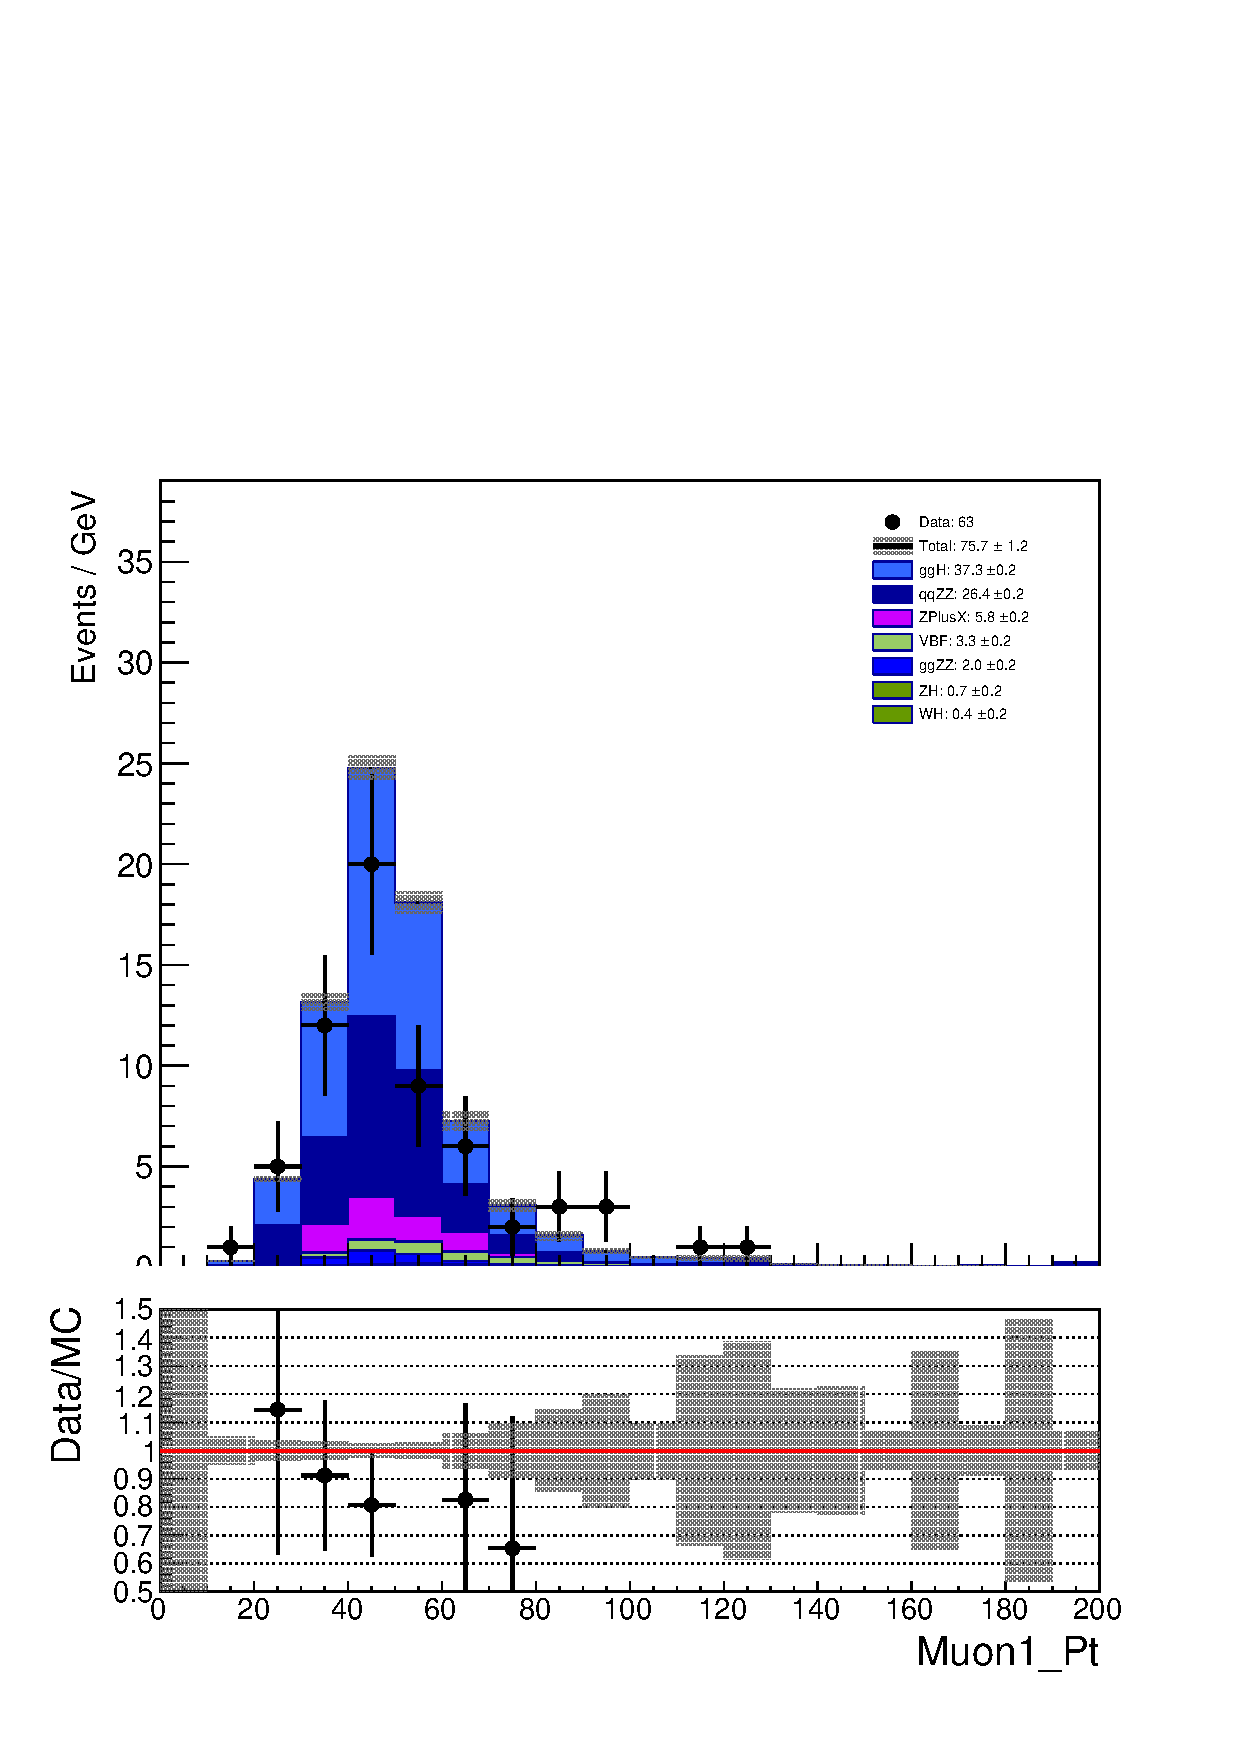
\includegraphics[width=0.49\textwidth]{Figures/Results/Distributions/DarkPhotonSR17/Muon1_Pt}}
{ 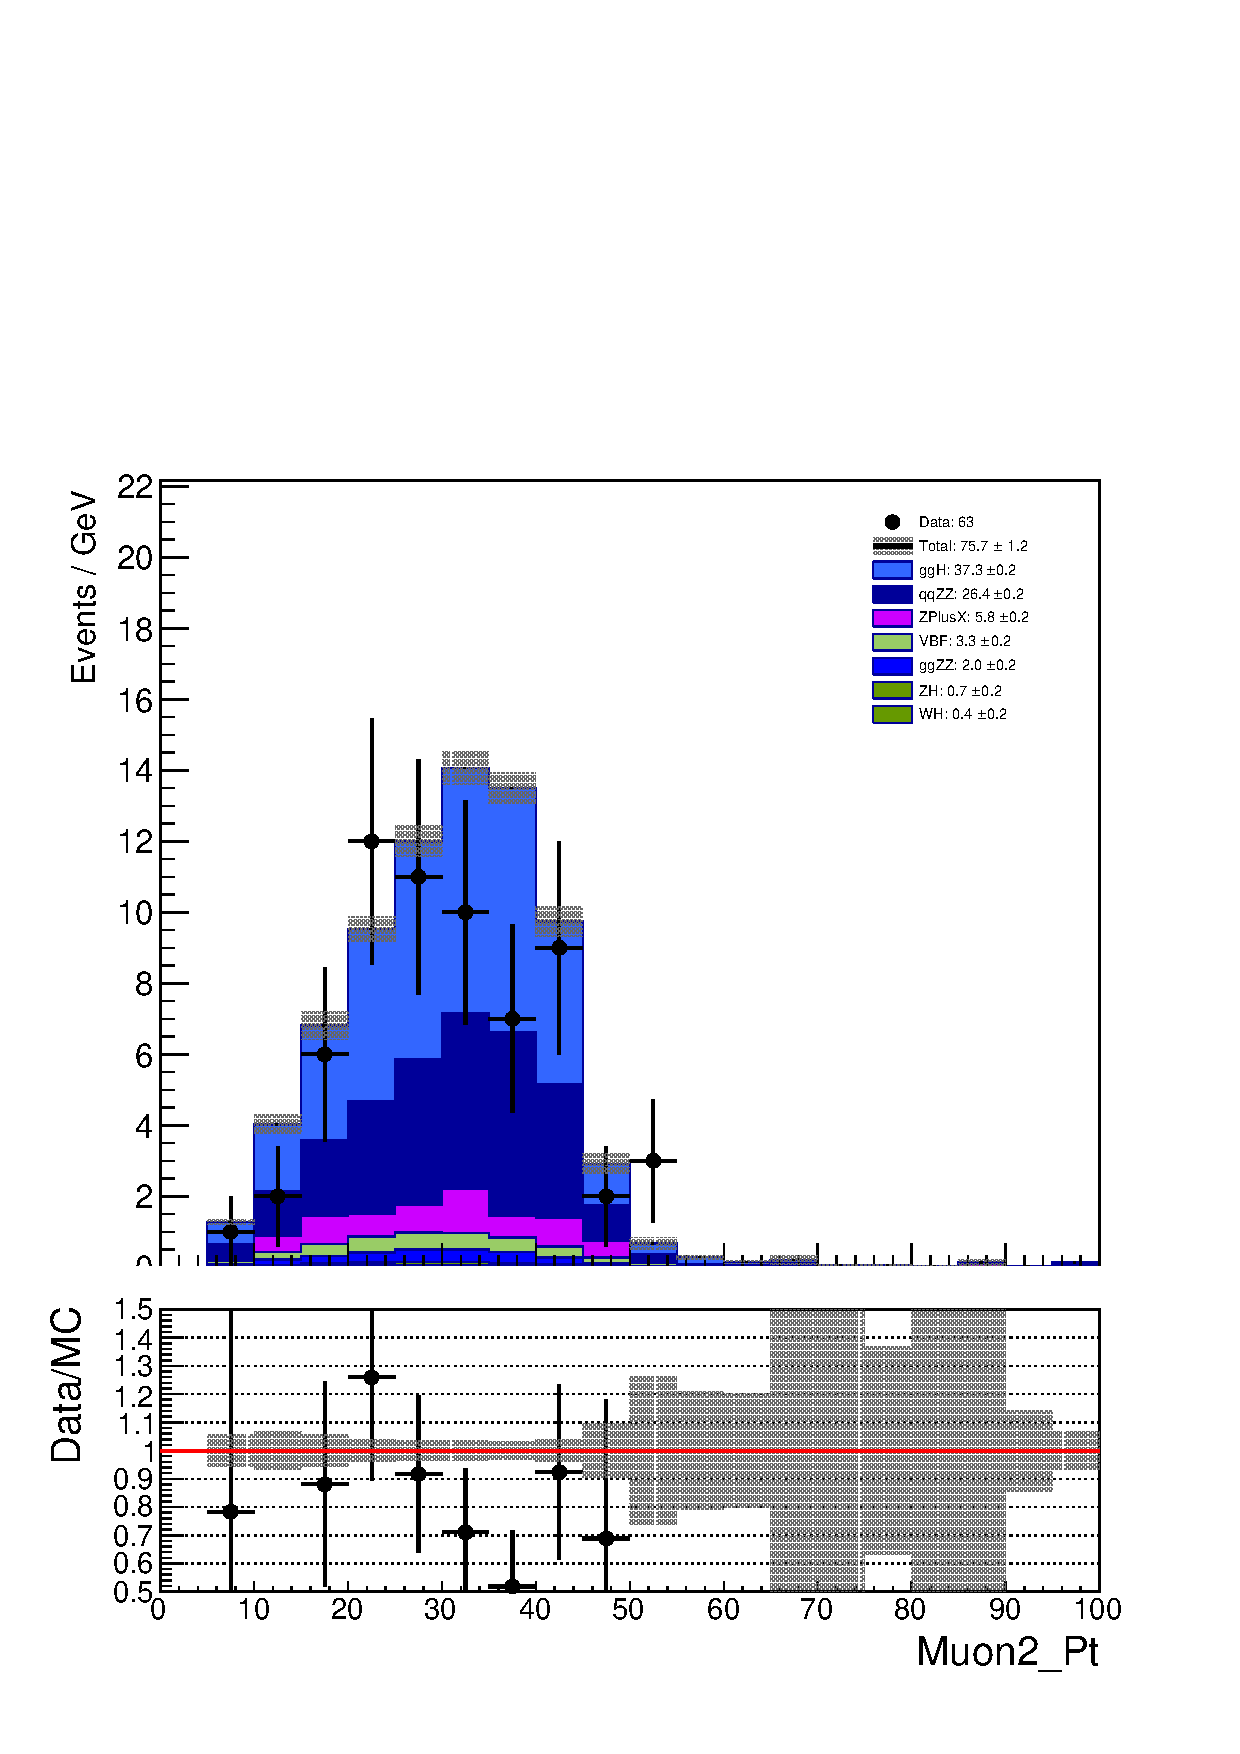
\includegraphics[width=0.49\textwidth]{Figures/Results/Distributions/DarkPhotonSR17/Muon2_Pt}}
{ 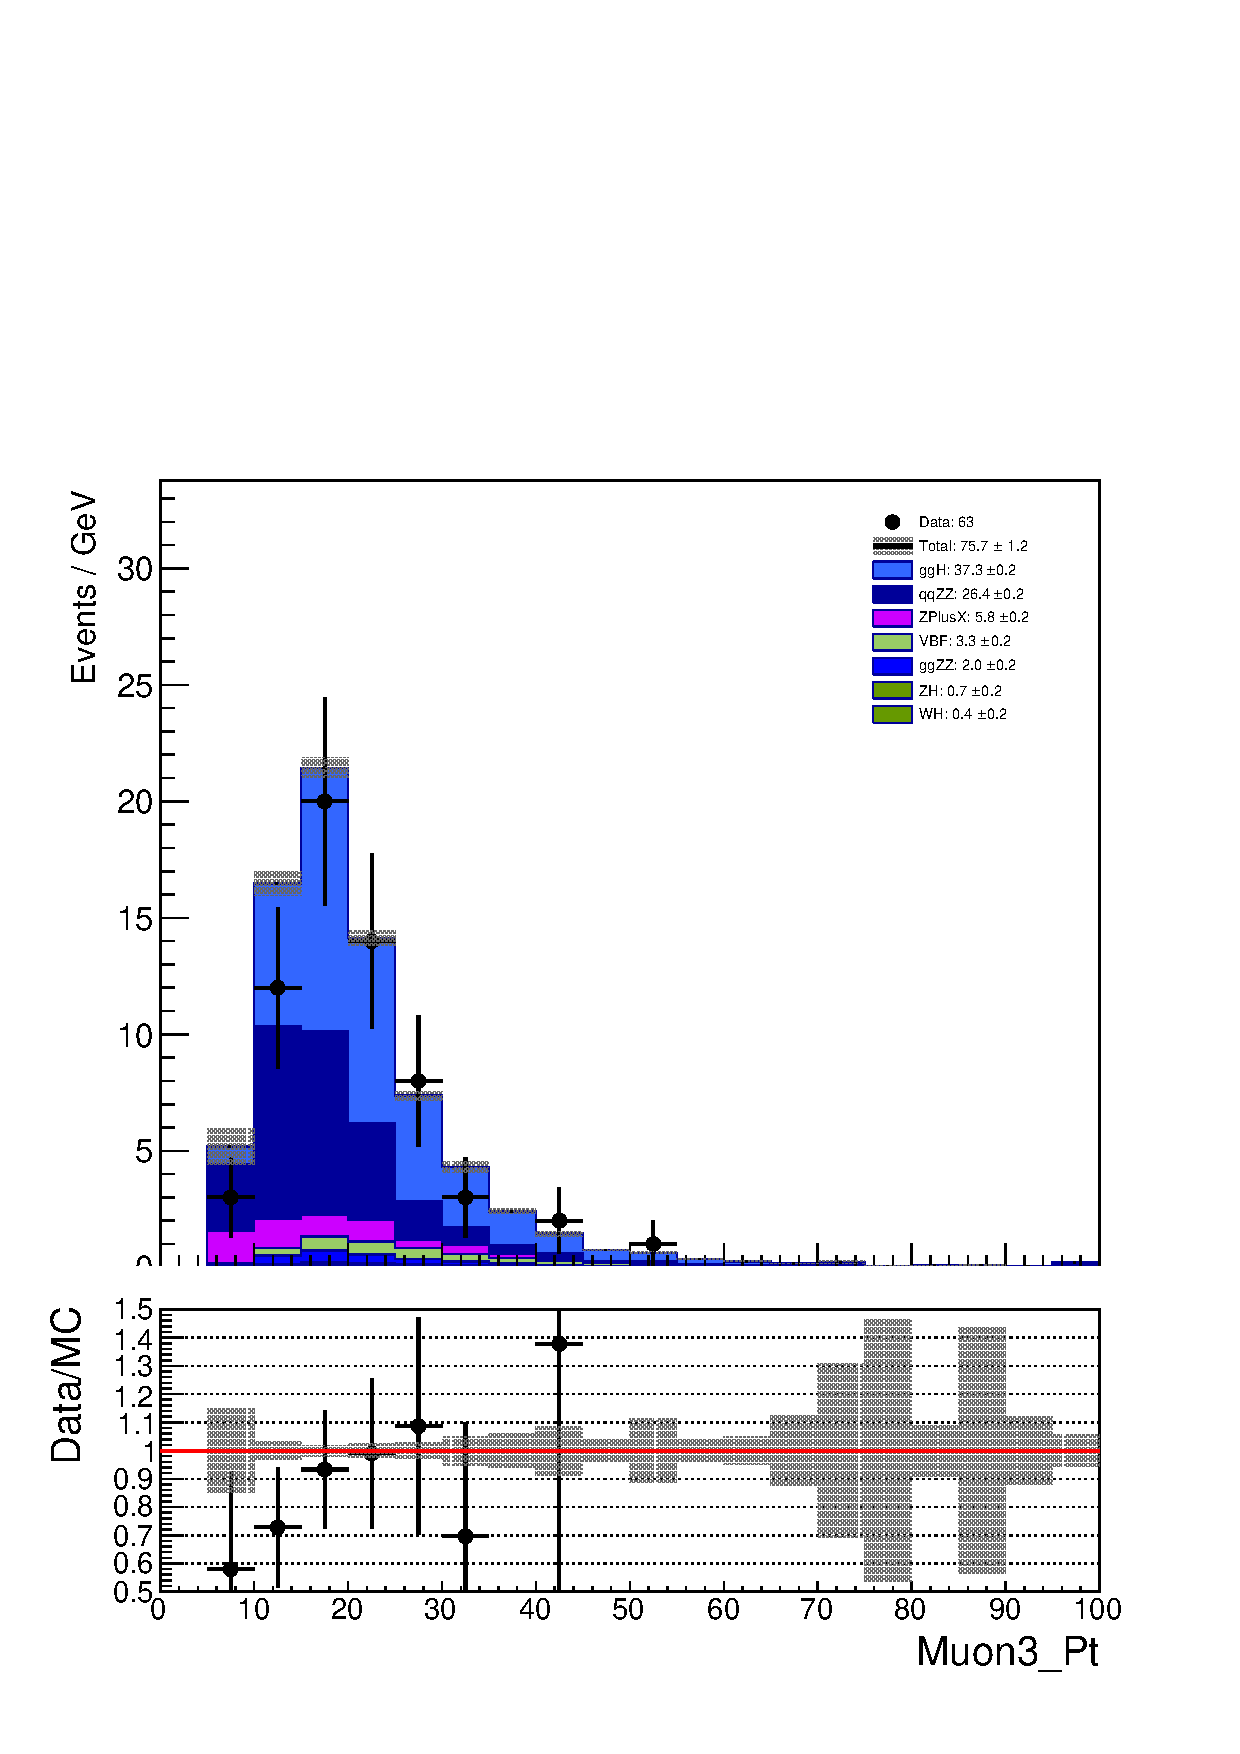
\includegraphics[width=0.49\textwidth]{Figures/Results/Distributions/DarkPhotonSR17/Muon3_Pt}}
{ 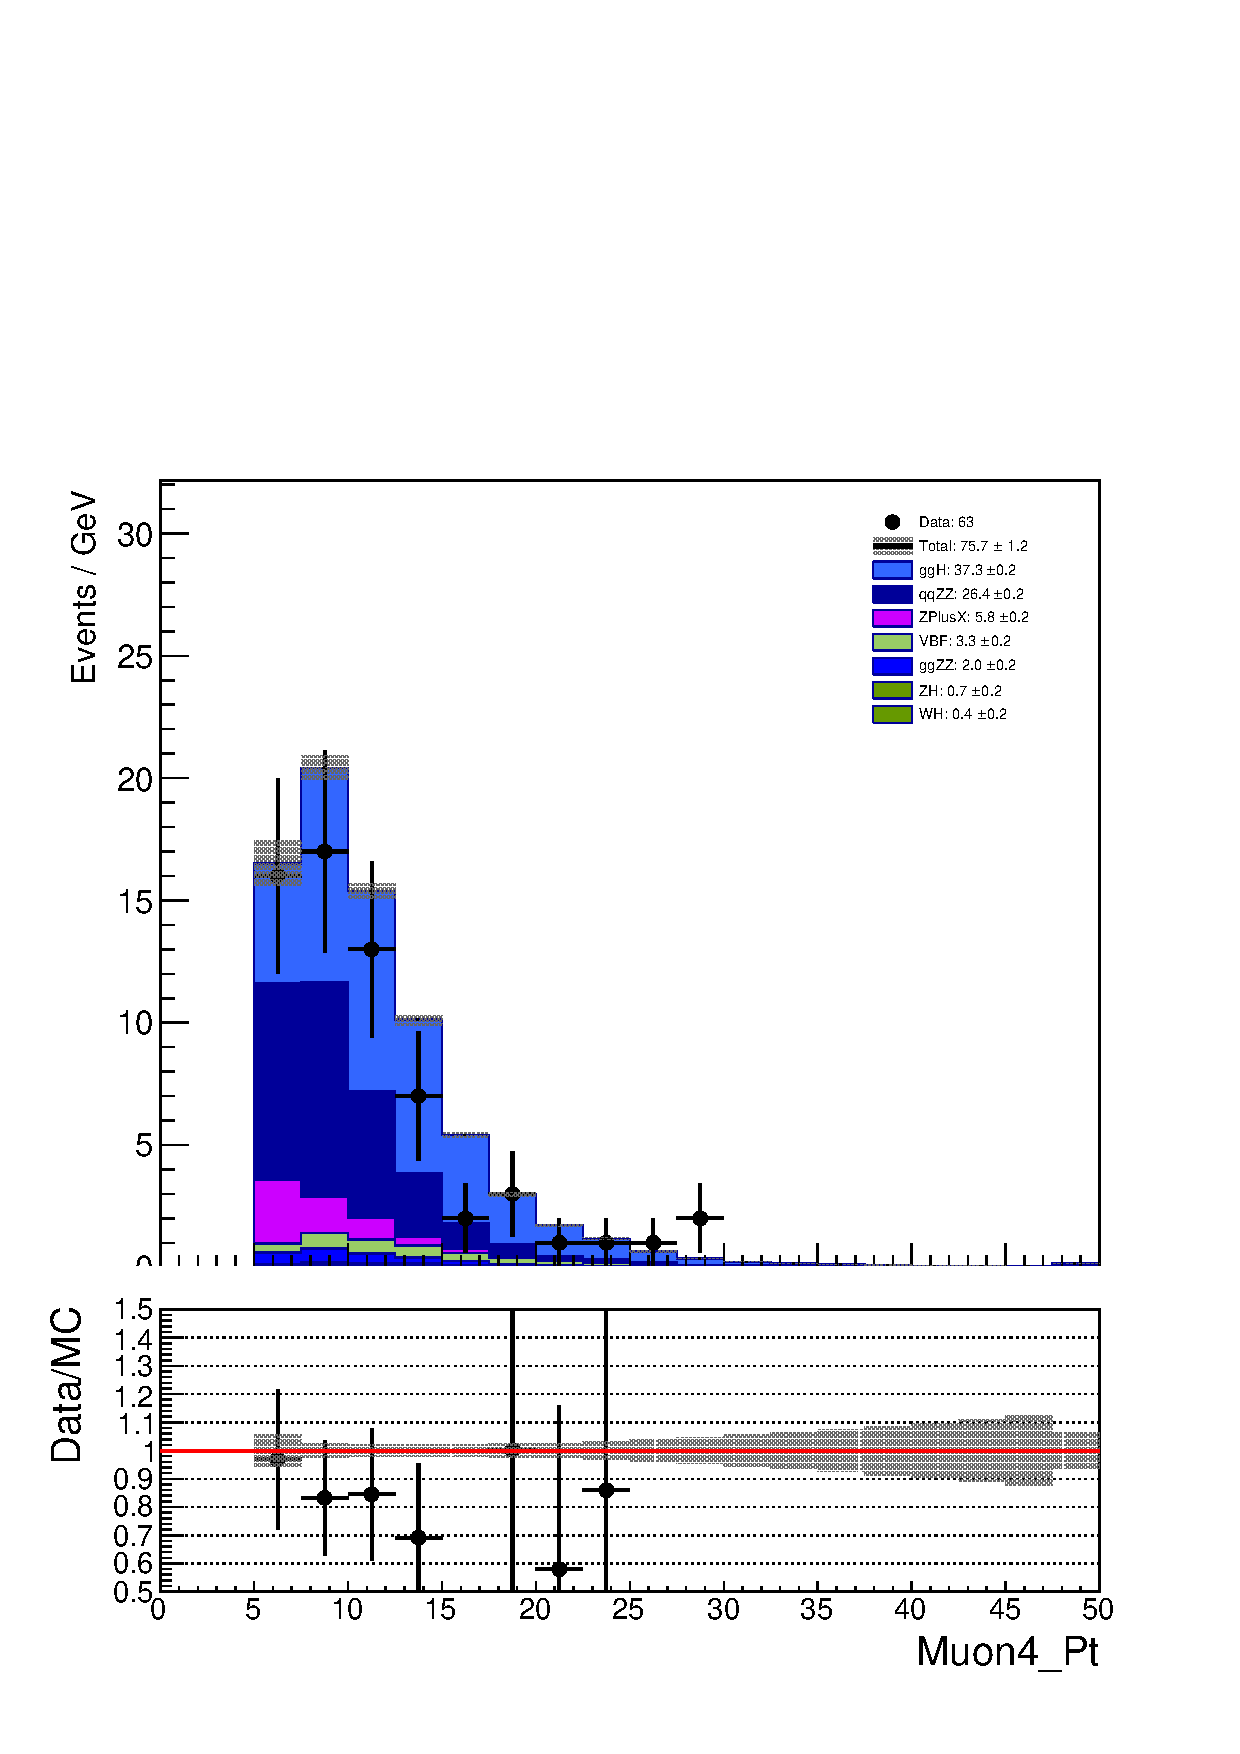
\includegraphics[width=0.49\textwidth]{Figures/Results/Distributions/DarkPhotonSR17/Muon4_Pt}}
\caption{ Distribution of the reconstructed muon~$\pt$ distribution and a comparison to predicted backgrounds using 2017 dataset.
\label{fig:muonPt_17}}
\end{figure}

\begin{figure}[!htbp]
\vspace*{0.3cm}
\centering
{ 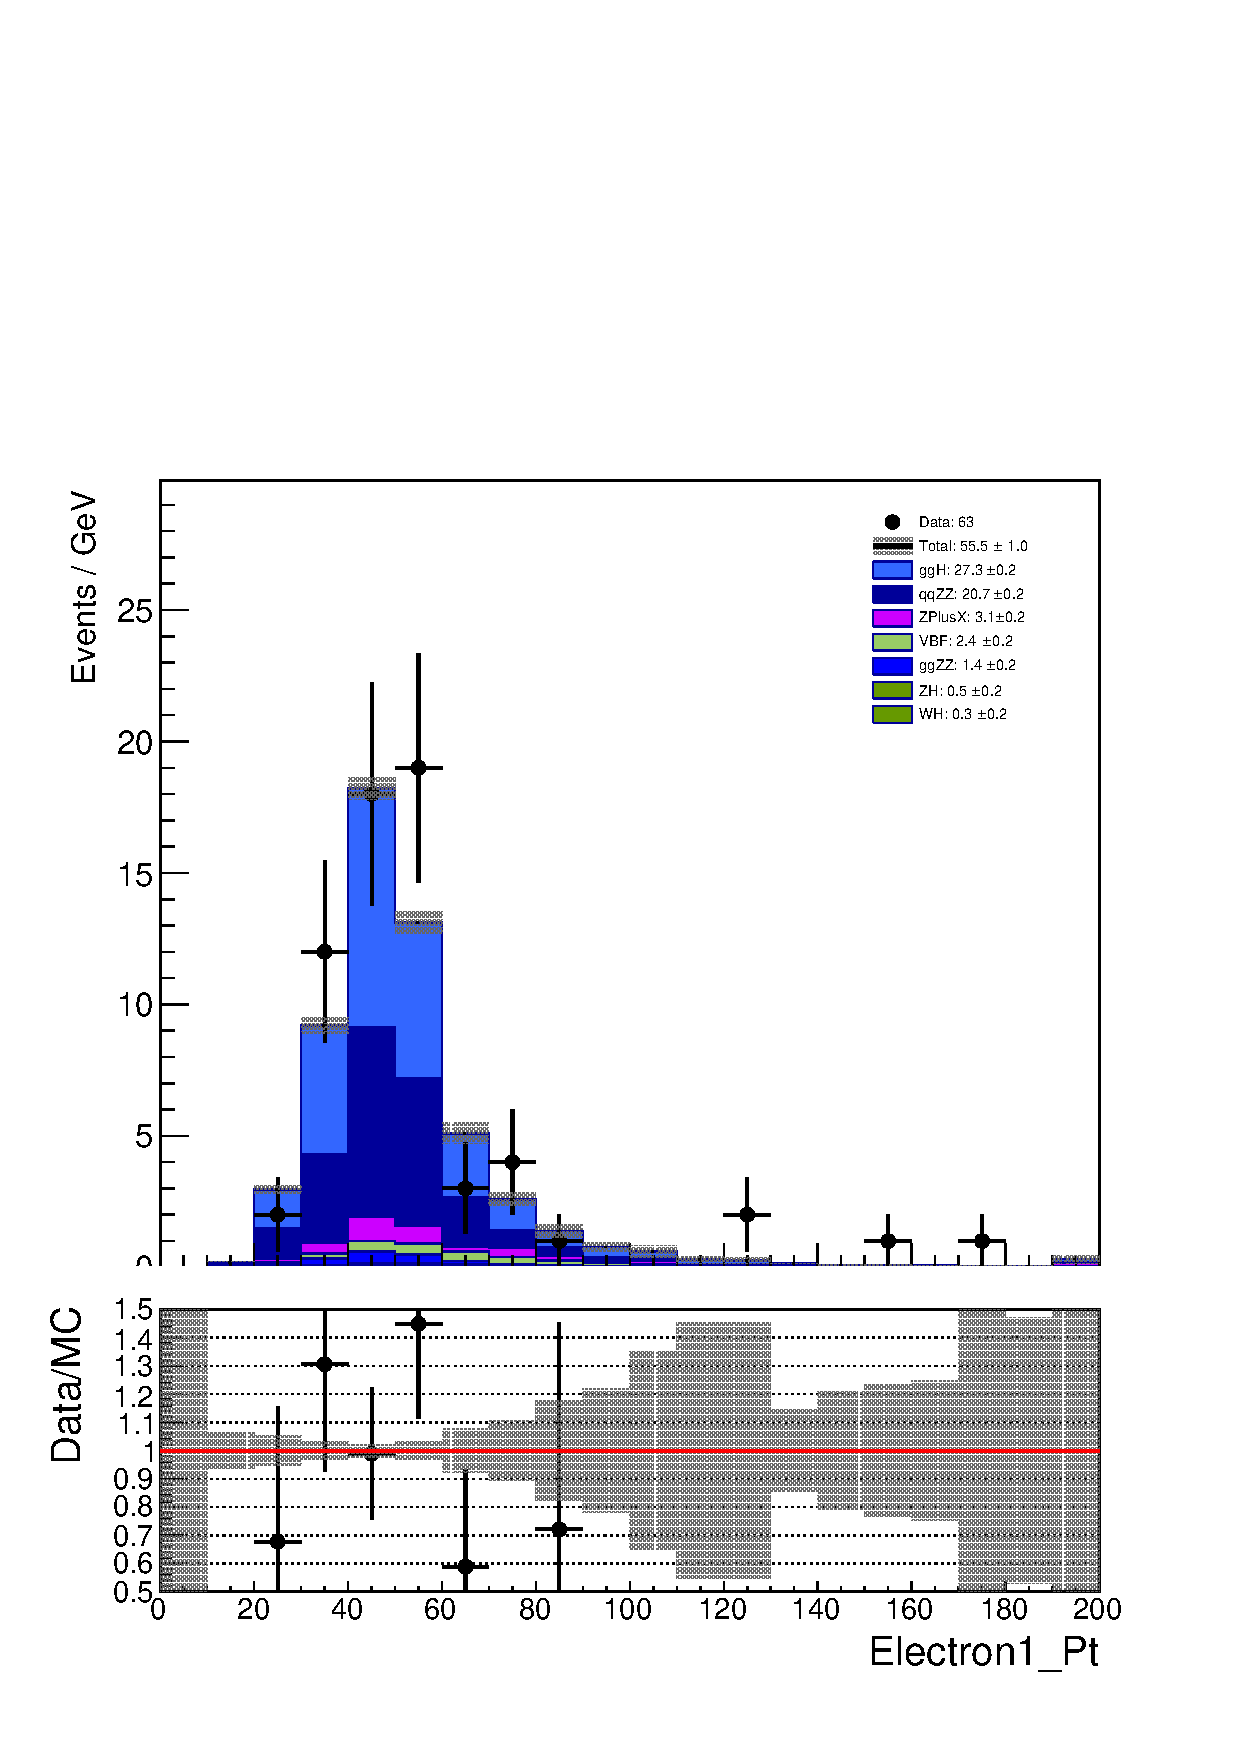
\includegraphics[width=0.49\textwidth]{Figures/Results/Distributions/DarkPhotonSR17/Electron1_Pt}}
{ 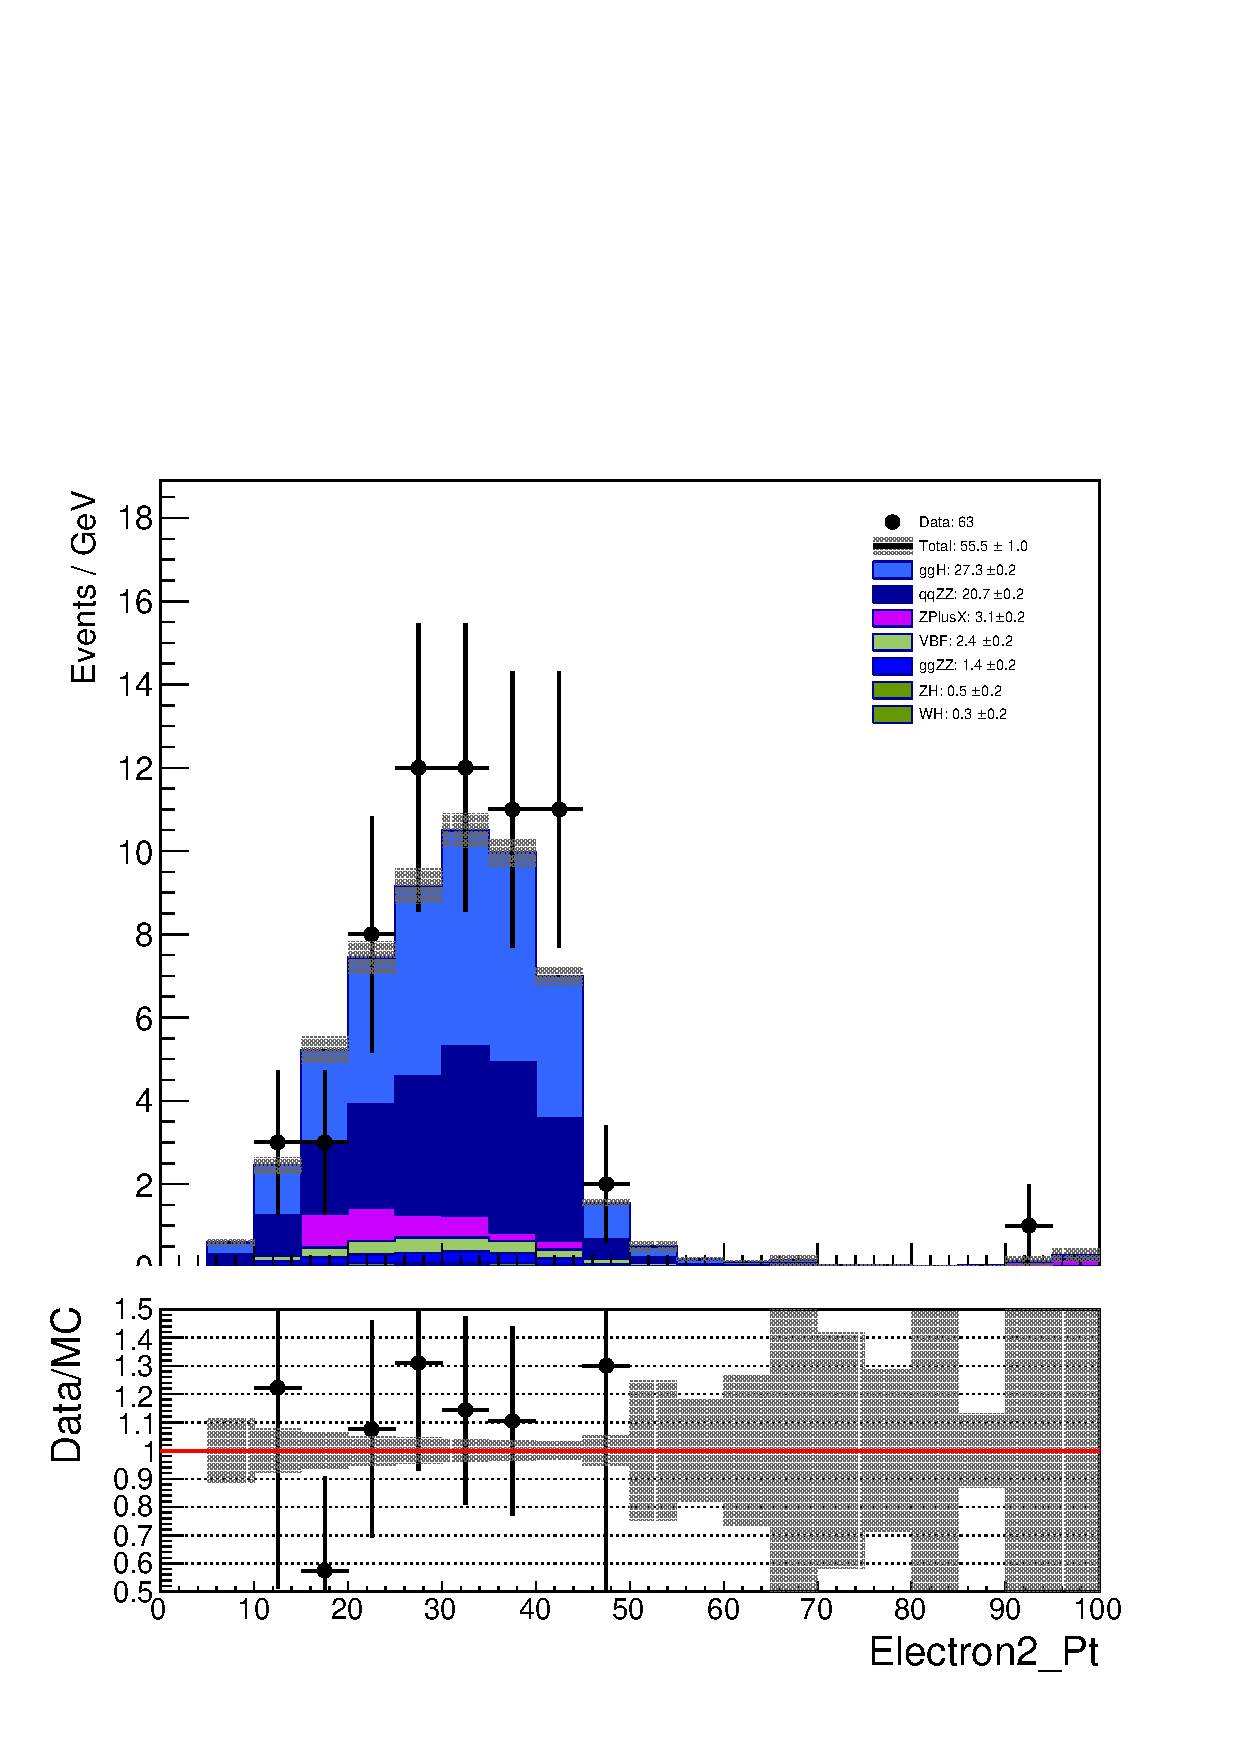
\includegraphics[width=0.49\textwidth]{Figures/Results/Distributions/DarkPhotonSR17/Electron2_Pt}}
{ 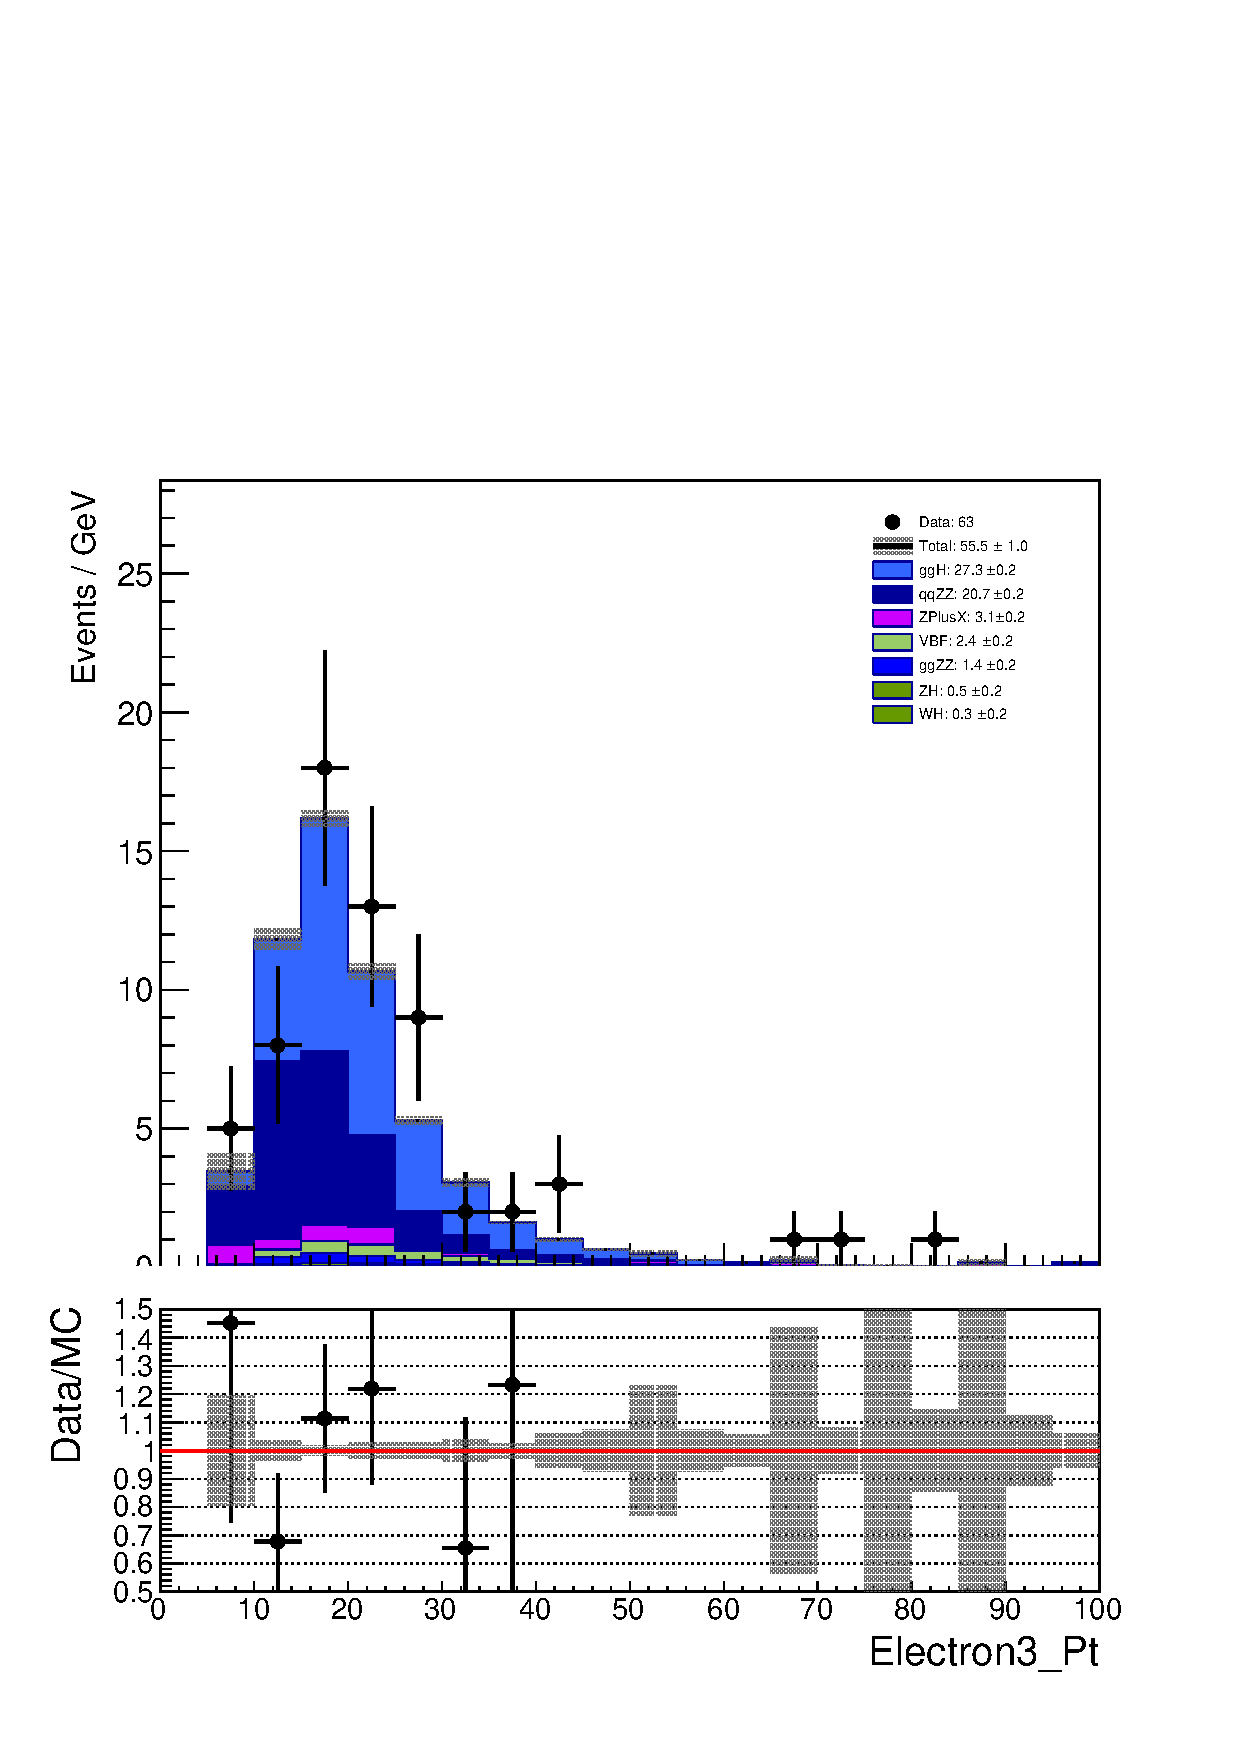
\includegraphics[width=0.49\textwidth]{Figures/Results/Distributions/DarkPhotonSR17/Electron3_Pt}}
{ 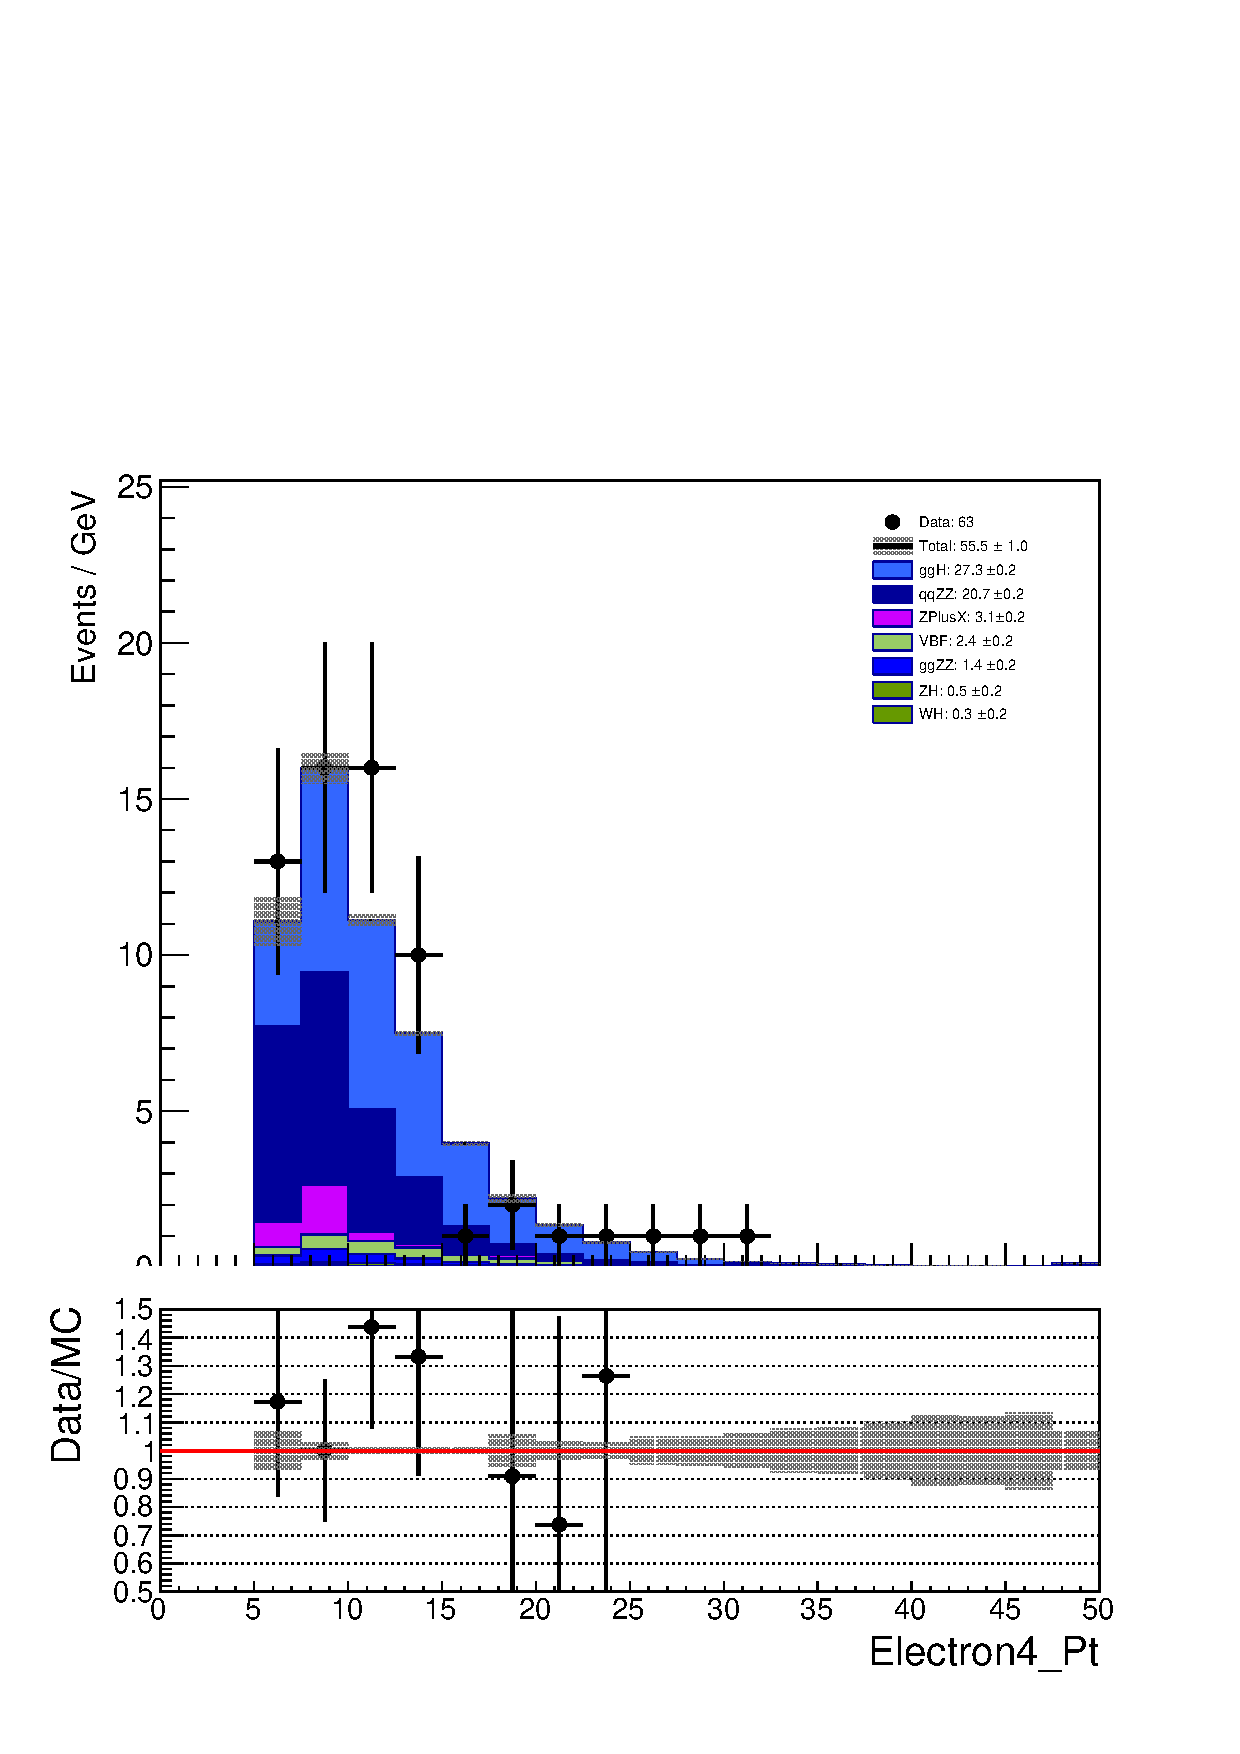
\includegraphics[width=0.49\textwidth]{Figures/Results/Distributions/DarkPhotonSR17/Electron4_Pt}}
\caption{ Distribution of the reconstructed electron~$\pt$ distribution and a comparison to predicted backgrounds using 2017 dataset.
\label{fig:elePt_17}}
\end{figure}

\begin{figure}[!htbp]
\vspace*{0.3cm}
\centering
{ 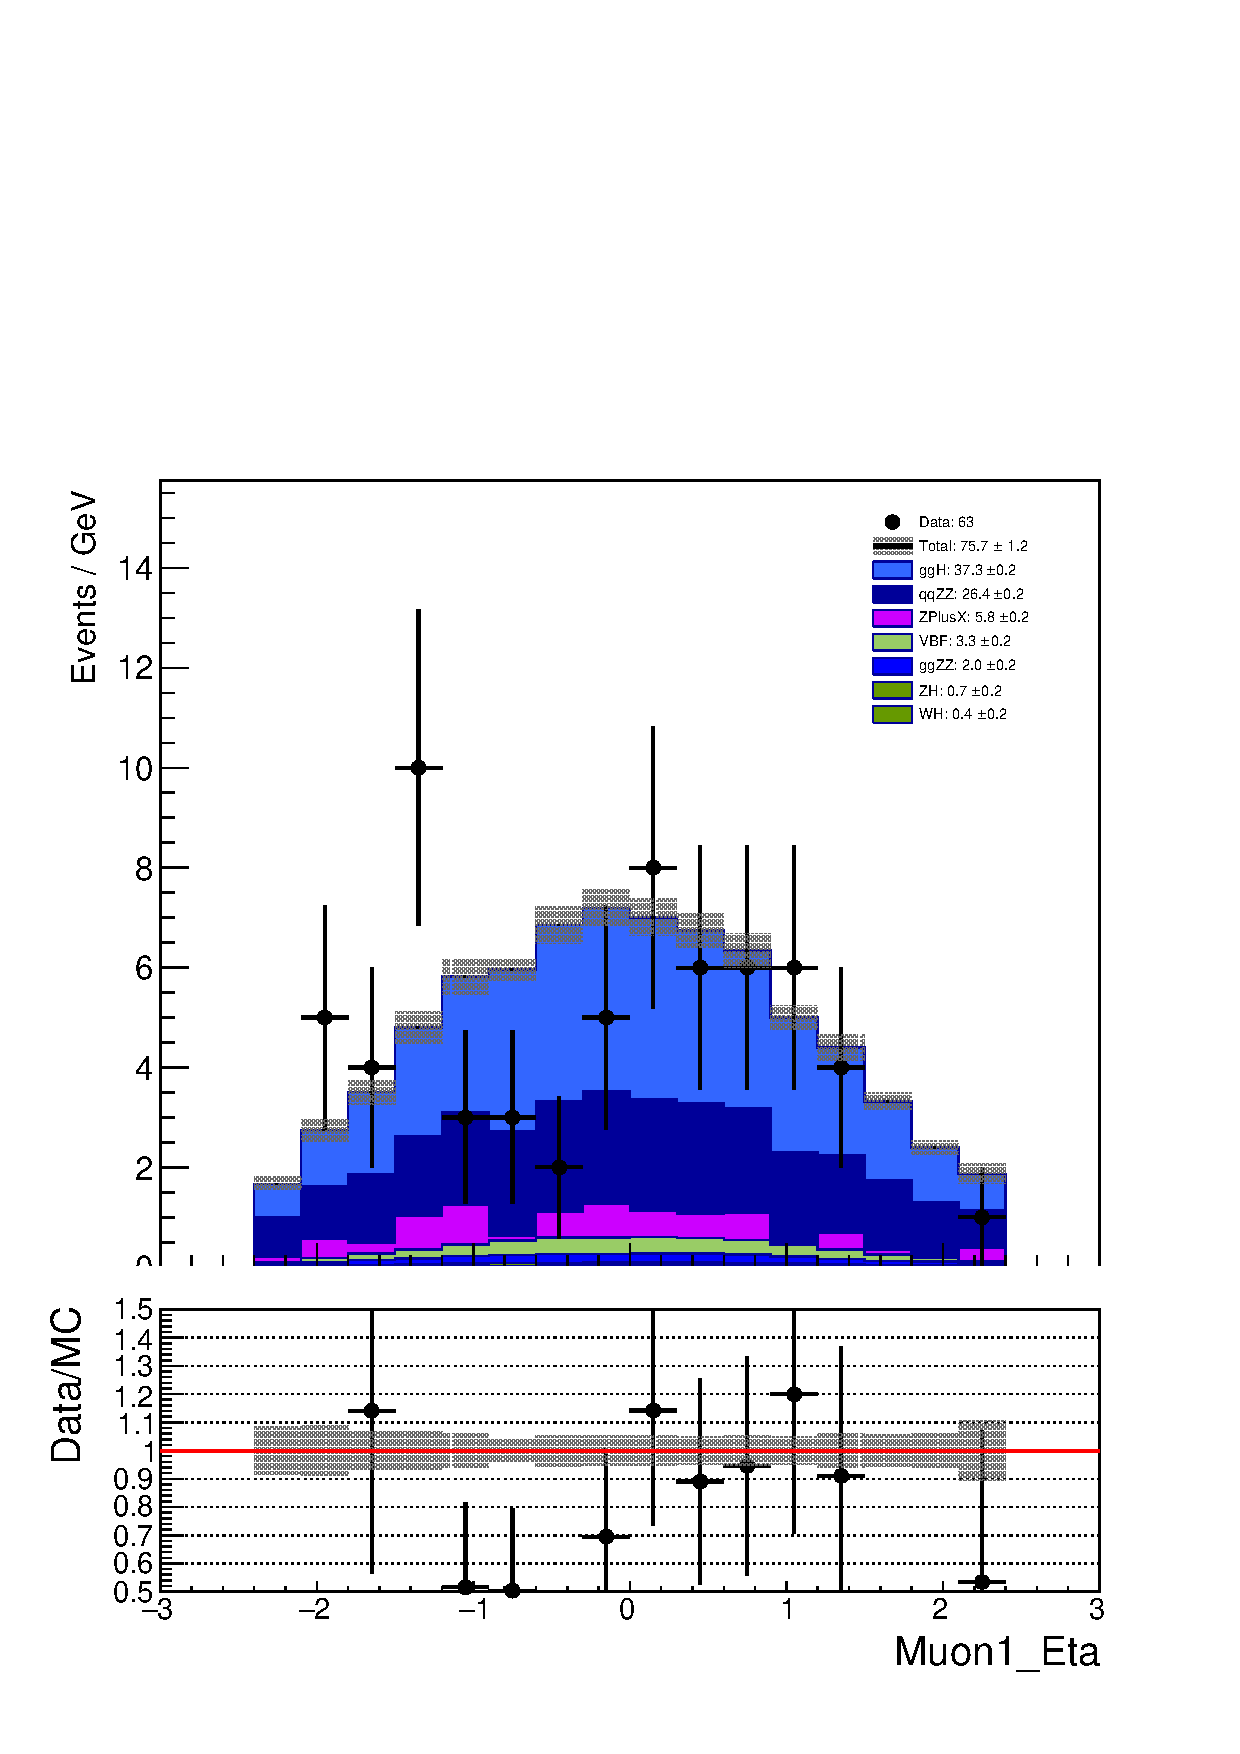
\includegraphics[width=0.49\textwidth]{Figures/Results/Distributions/DarkPhotonSR17/Muon1_Eta}}
{ 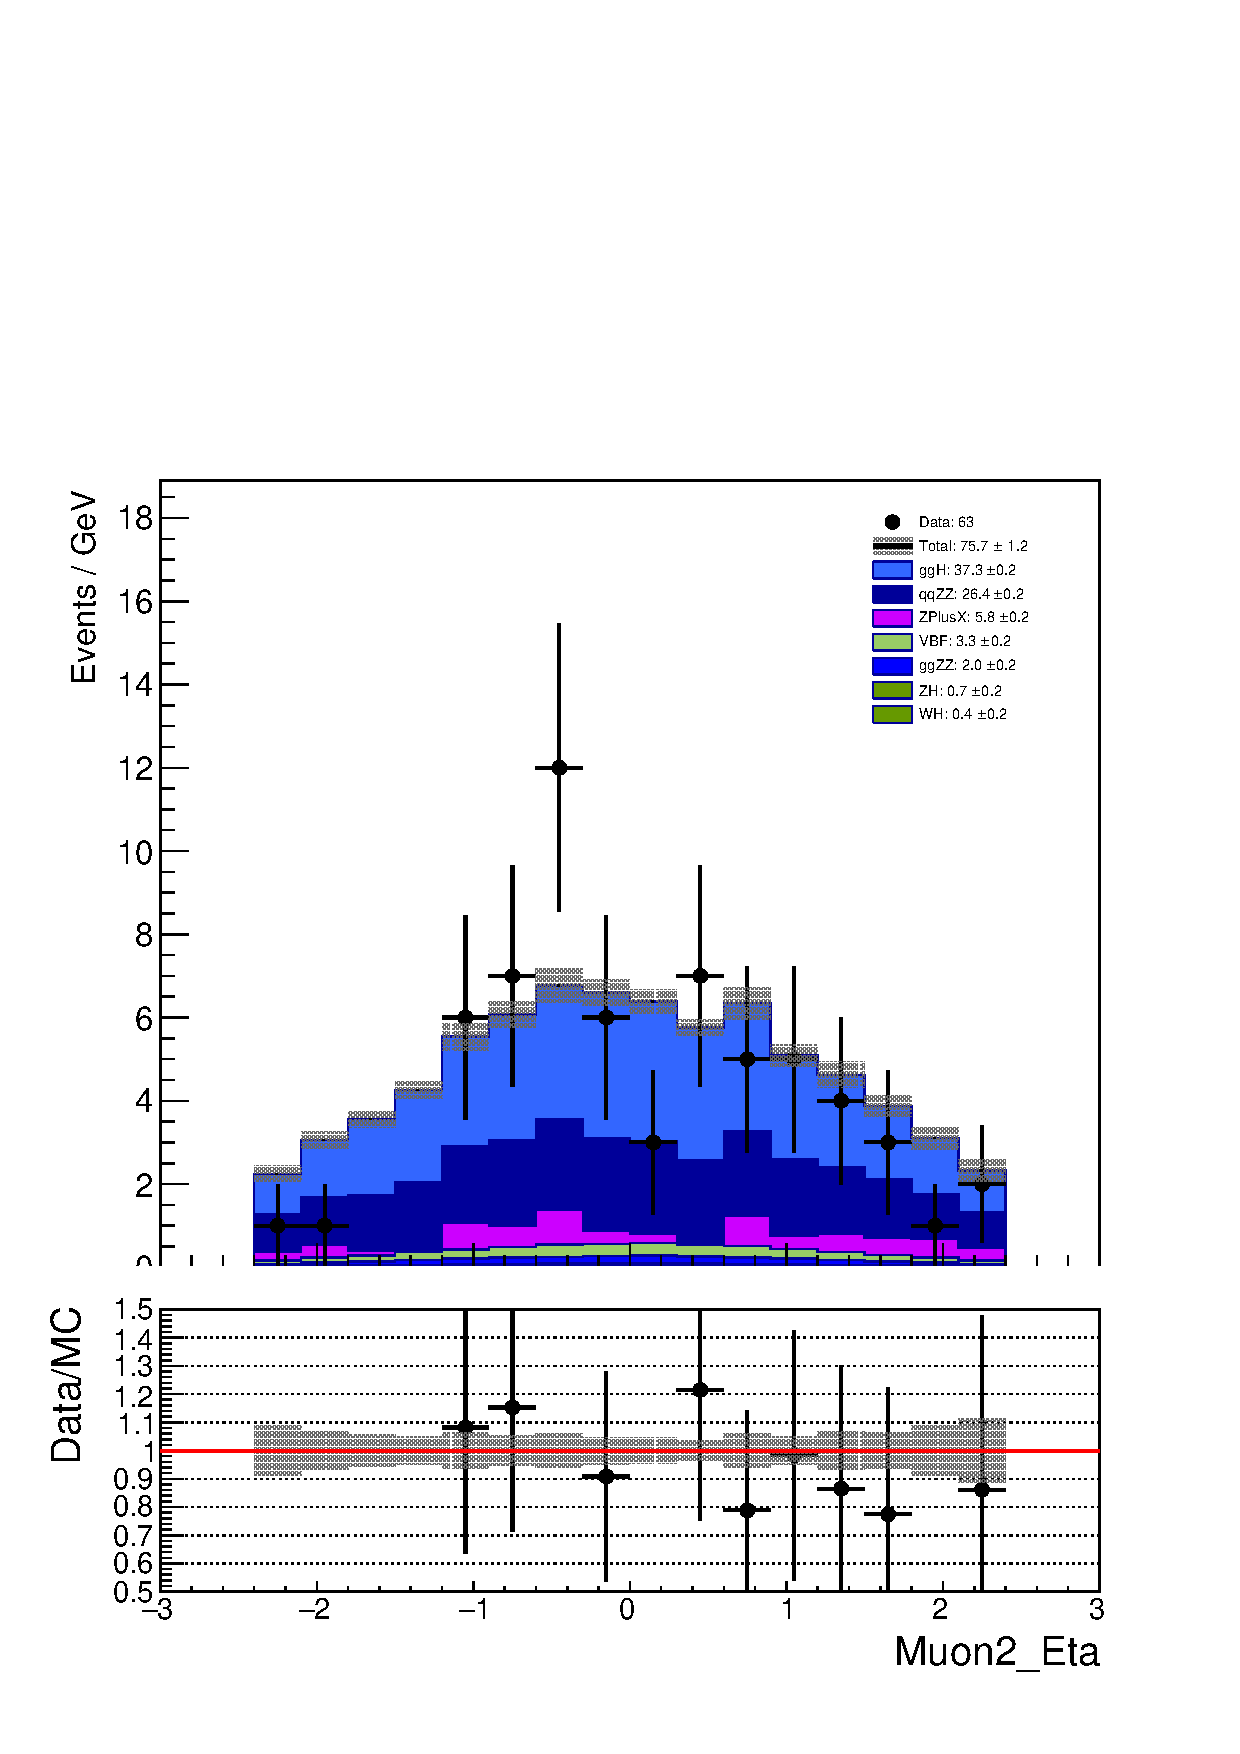
\includegraphics[width=0.49\textwidth]{Figures/Results/Distributions/DarkPhotonSR17/Muon2_Eta}}
{ 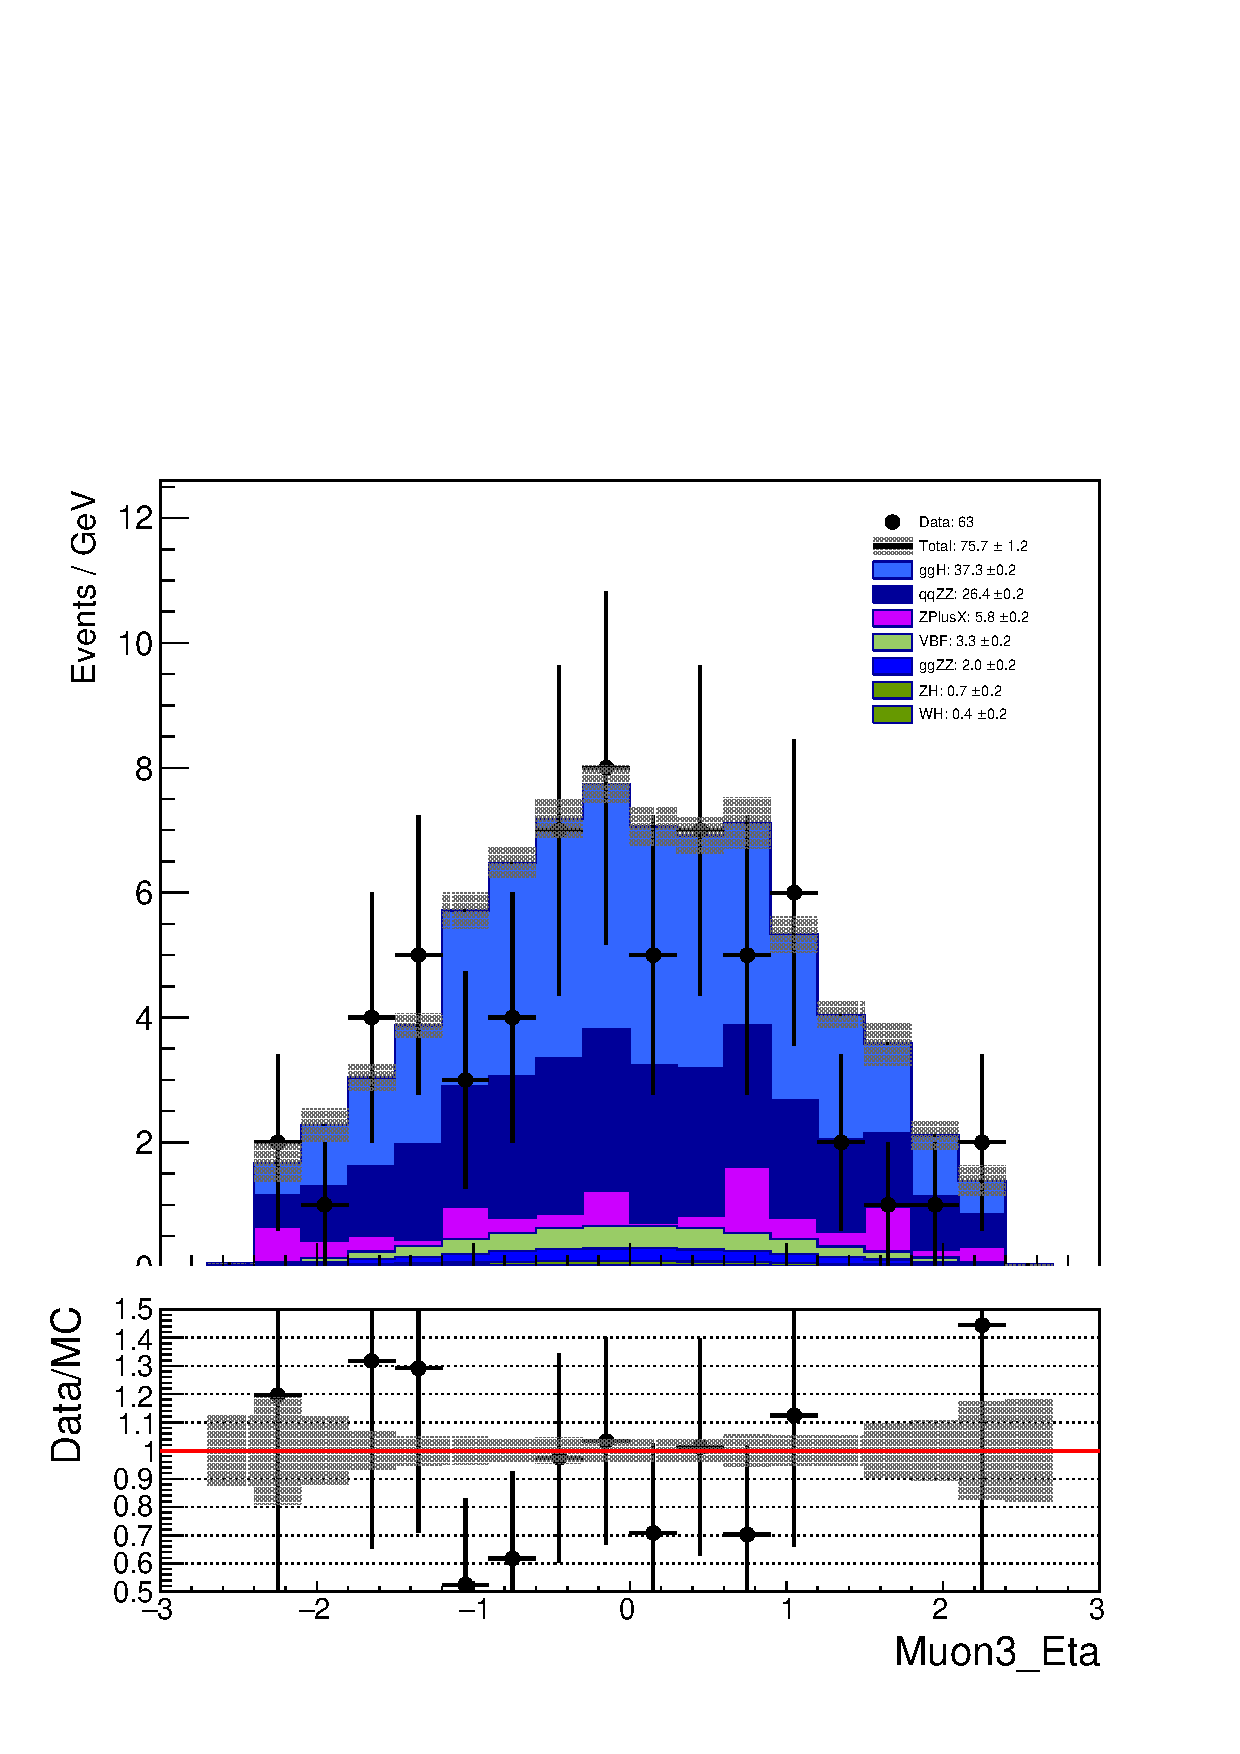
\includegraphics[width=0.49\textwidth]{Figures/Results/Distributions/DarkPhotonSR17/Muon3_Eta}}
{ 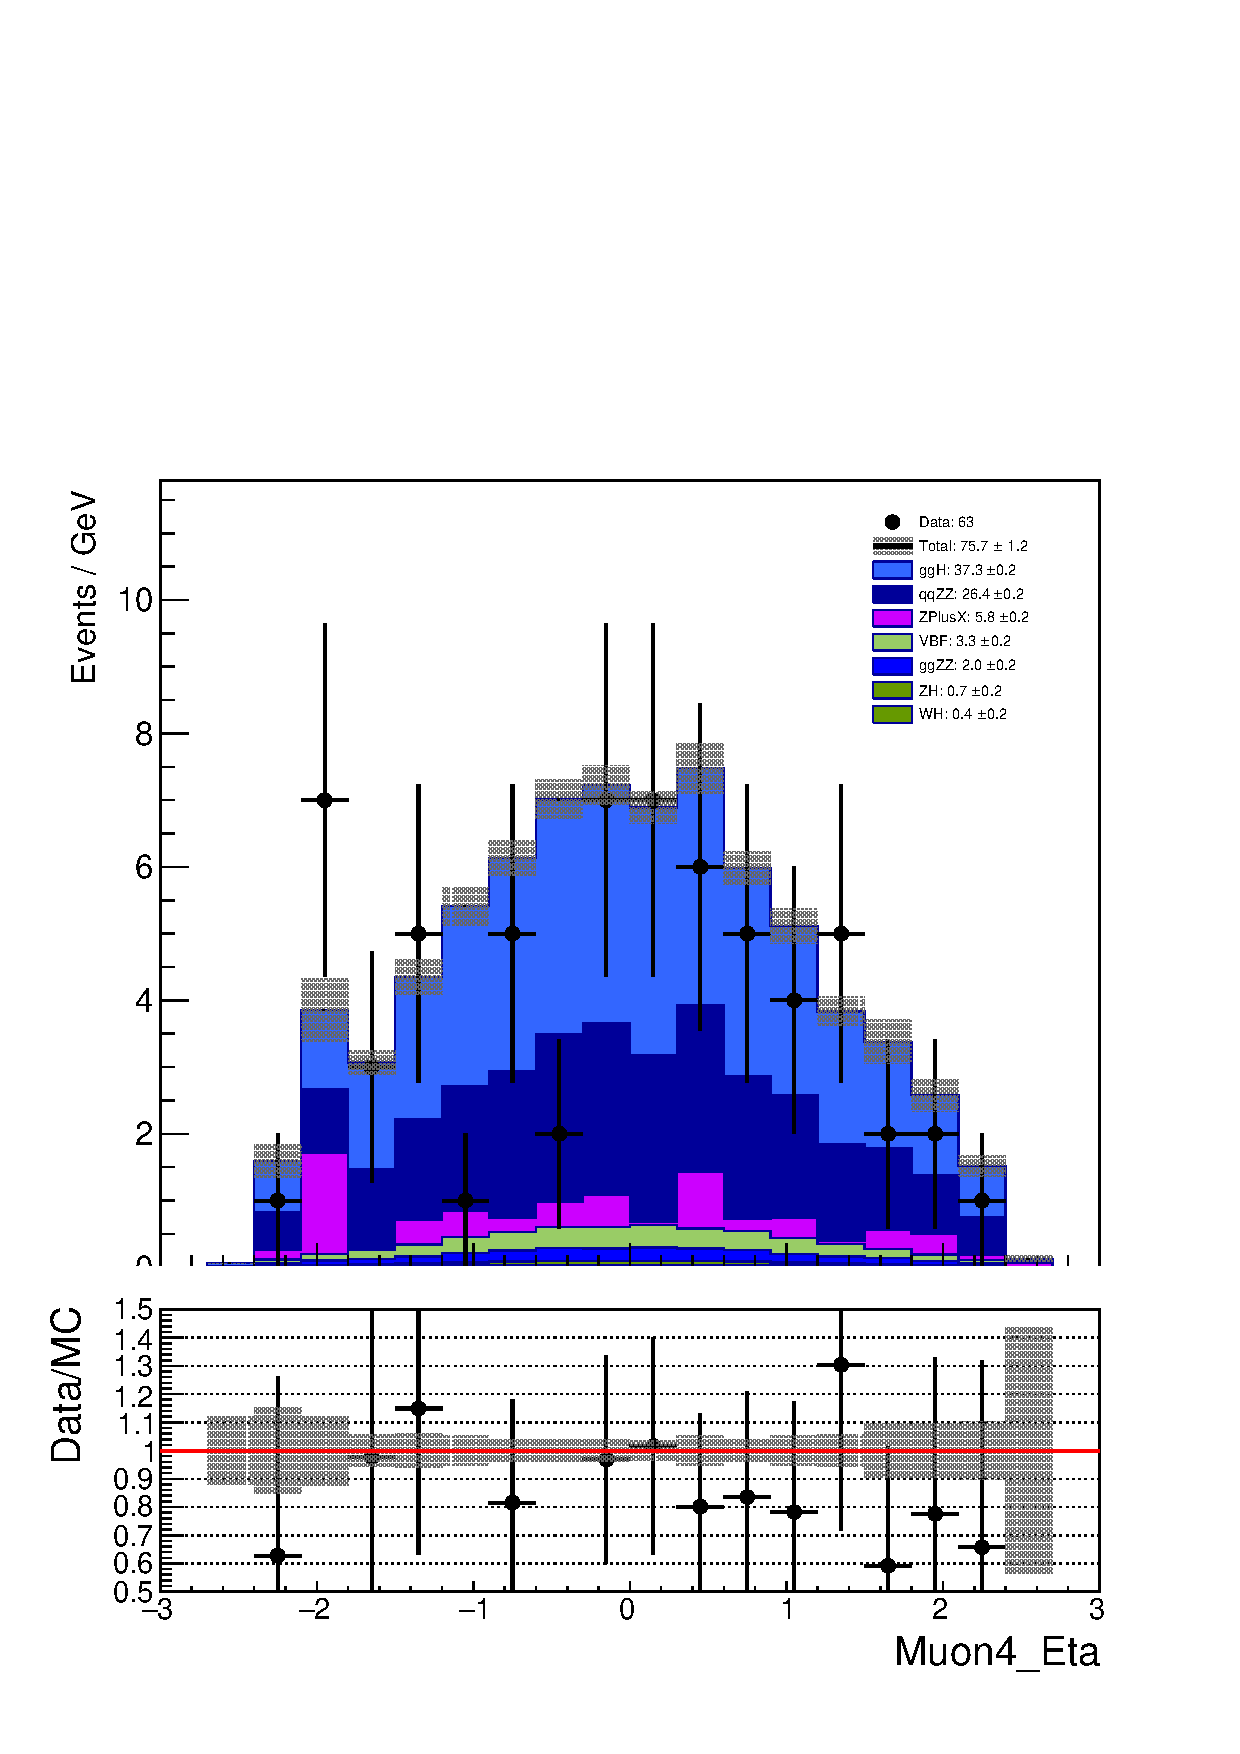
\includegraphics[width=0.49\textwidth]{Figures/Results/Distributions/DarkPhotonSR17/Muon4_Eta}}
\caption{ Distribution of the reconstructed muon~$\eta$ distribution and a comparison to predicted backgrounds using 2017 dataset.
\label{fig:muonEta_17}}
\end{figure}

\begin{figure}[!htbp]
\vspace*{0.3cm}
\centering
{ 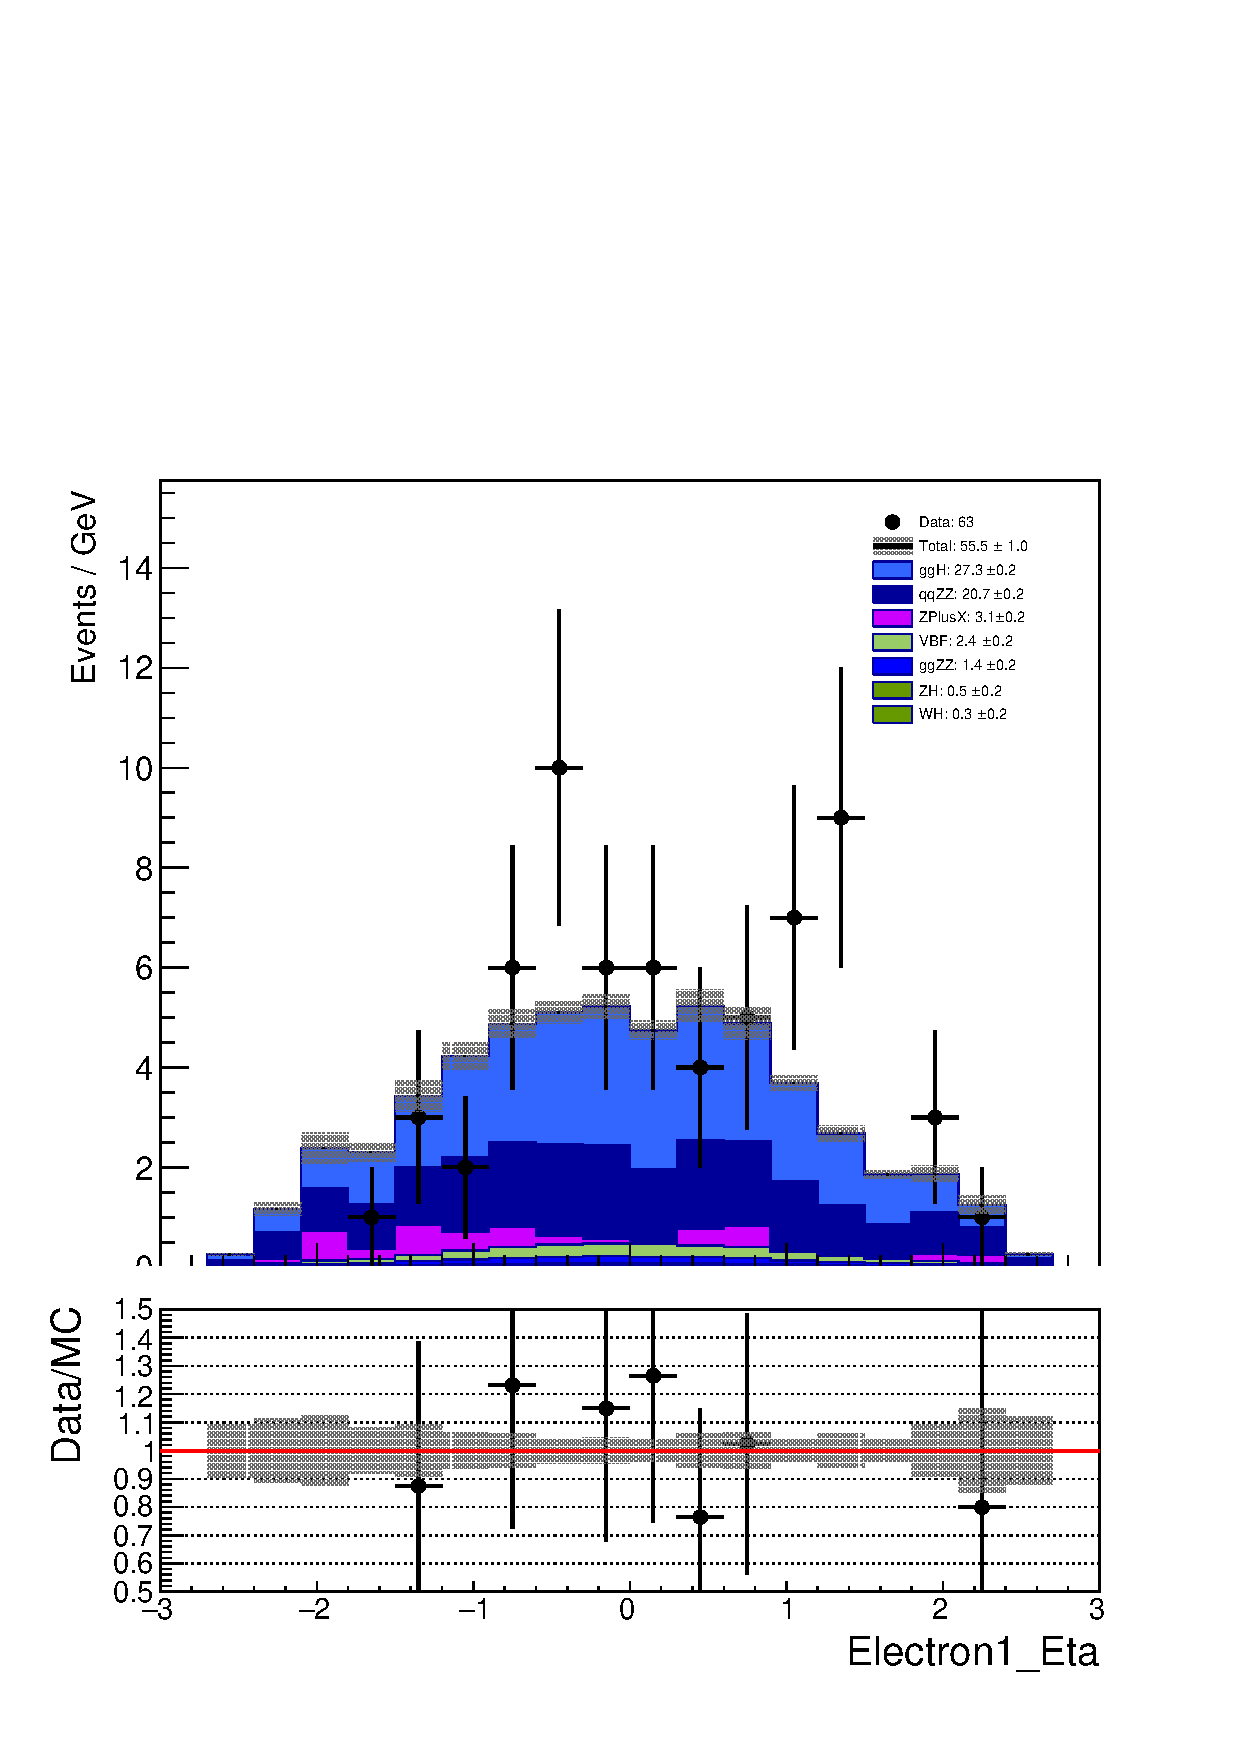
\includegraphics[width=0.49\textwidth]{Figures/Results/Distributions/DarkPhotonSR17/Electron1_Eta}}
{ 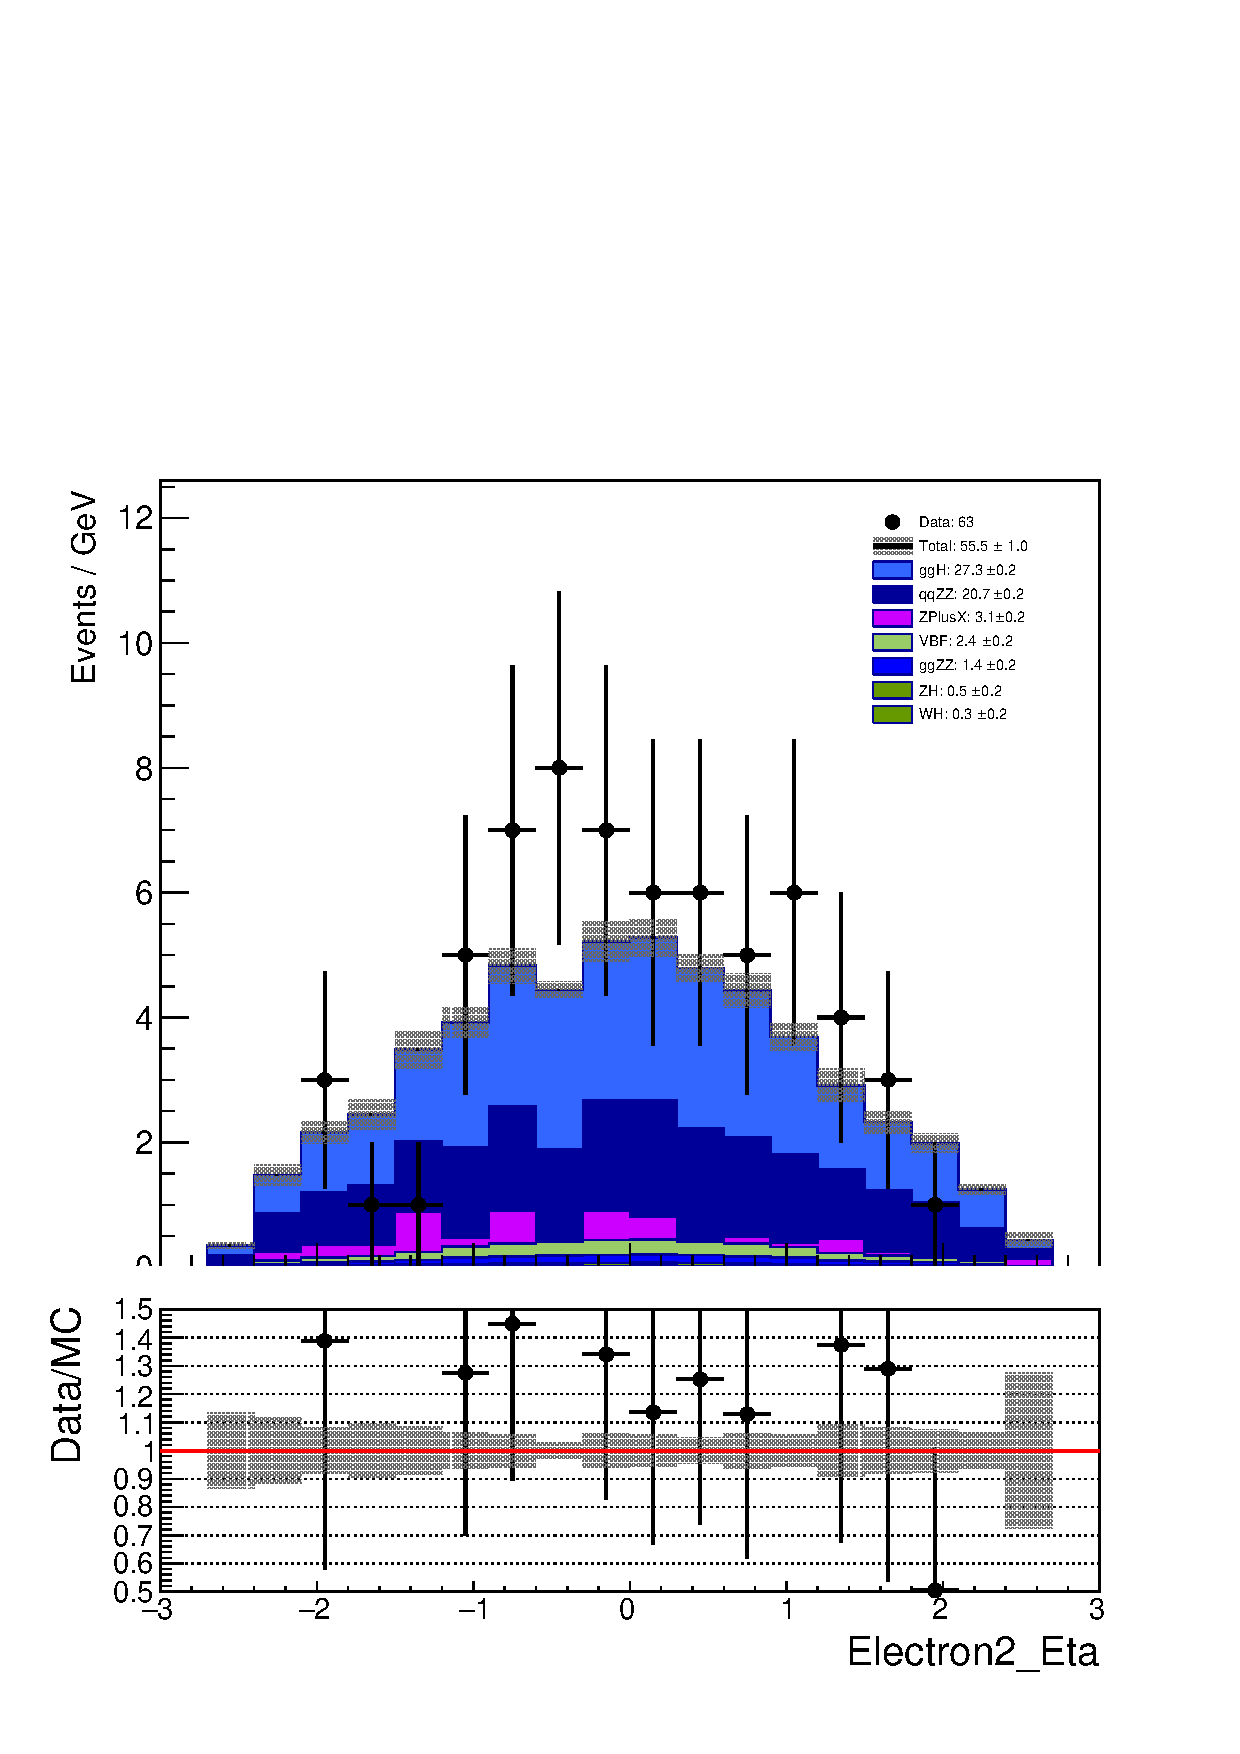
\includegraphics[width=0.49\textwidth]{Figures/Results/Distributions/DarkPhotonSR17/Electron2_Eta}}
{ 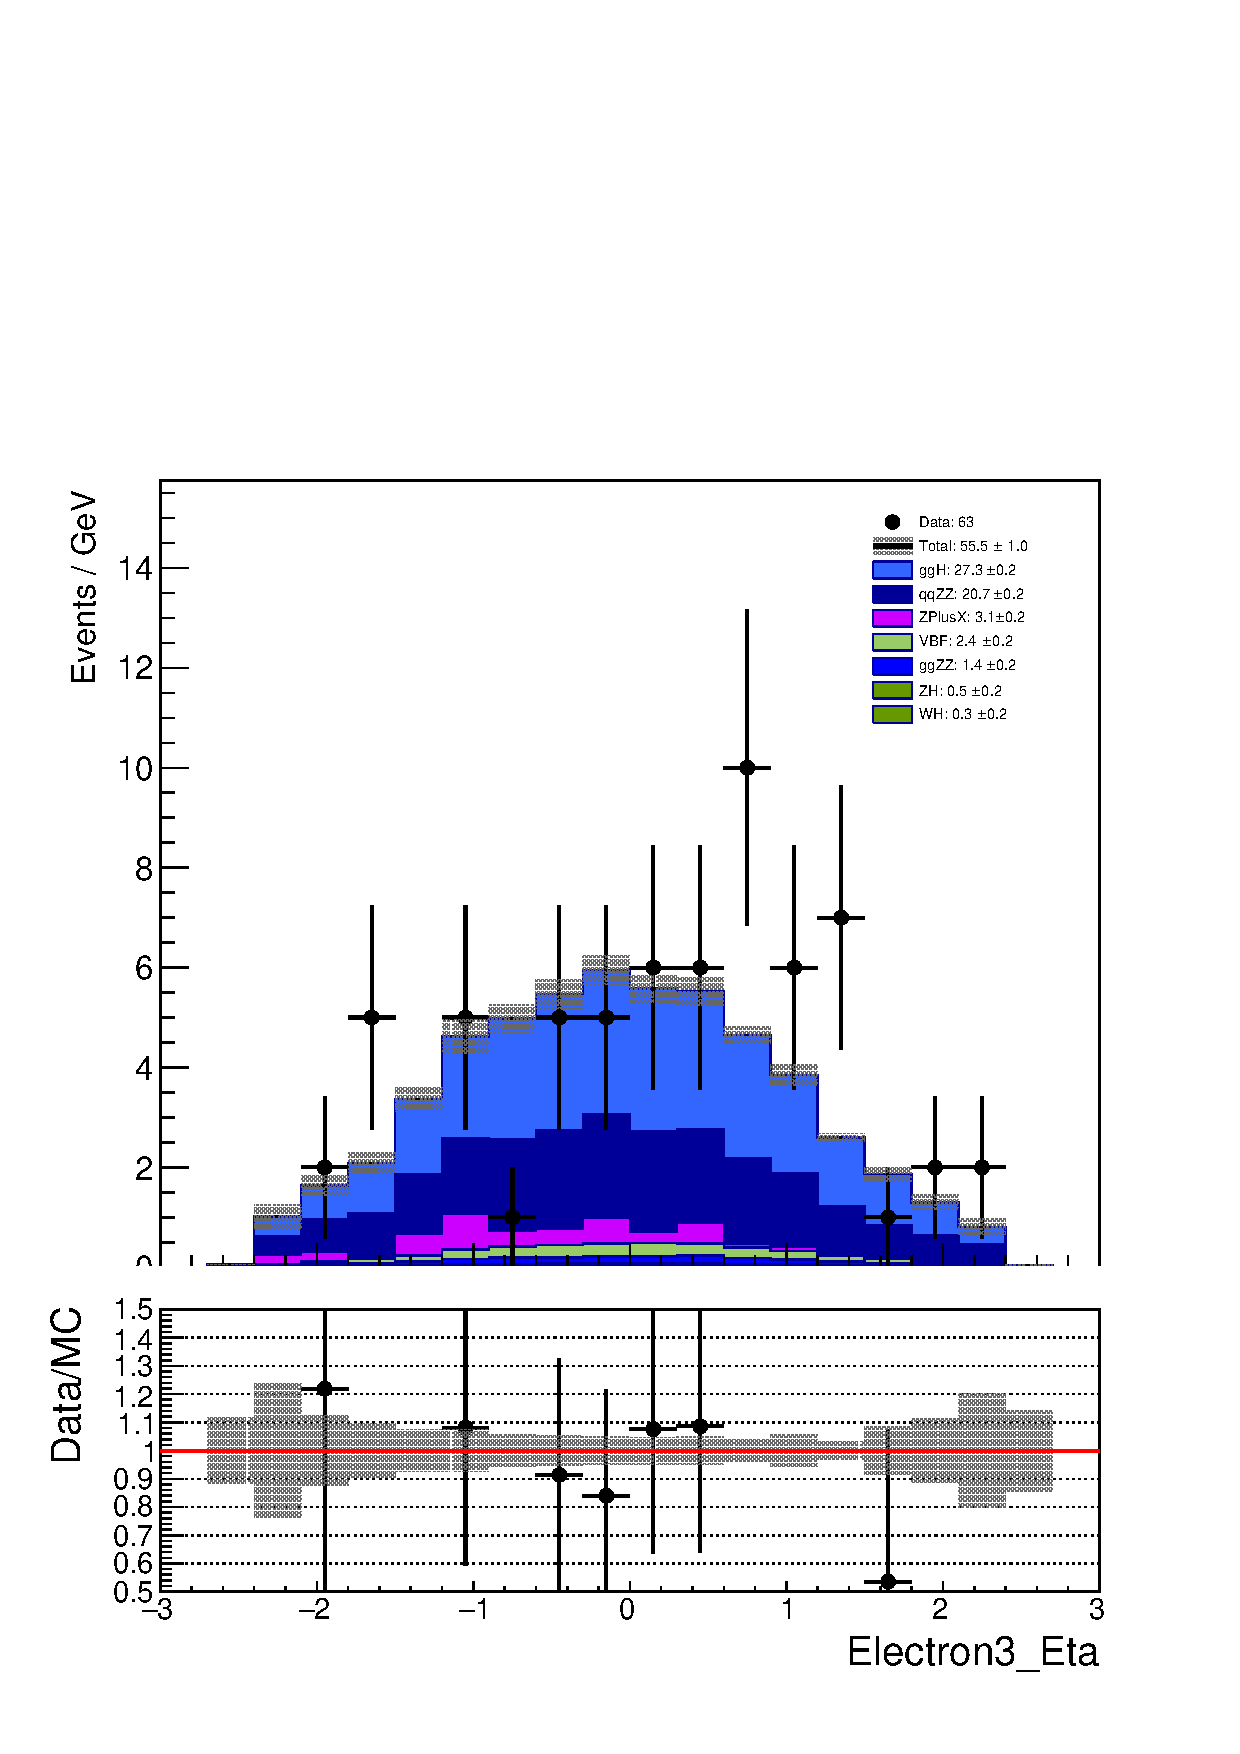
\includegraphics[width=0.49\textwidth]{Figures/Results/Distributions/DarkPhotonSR17/Electron3_Eta}}
{ 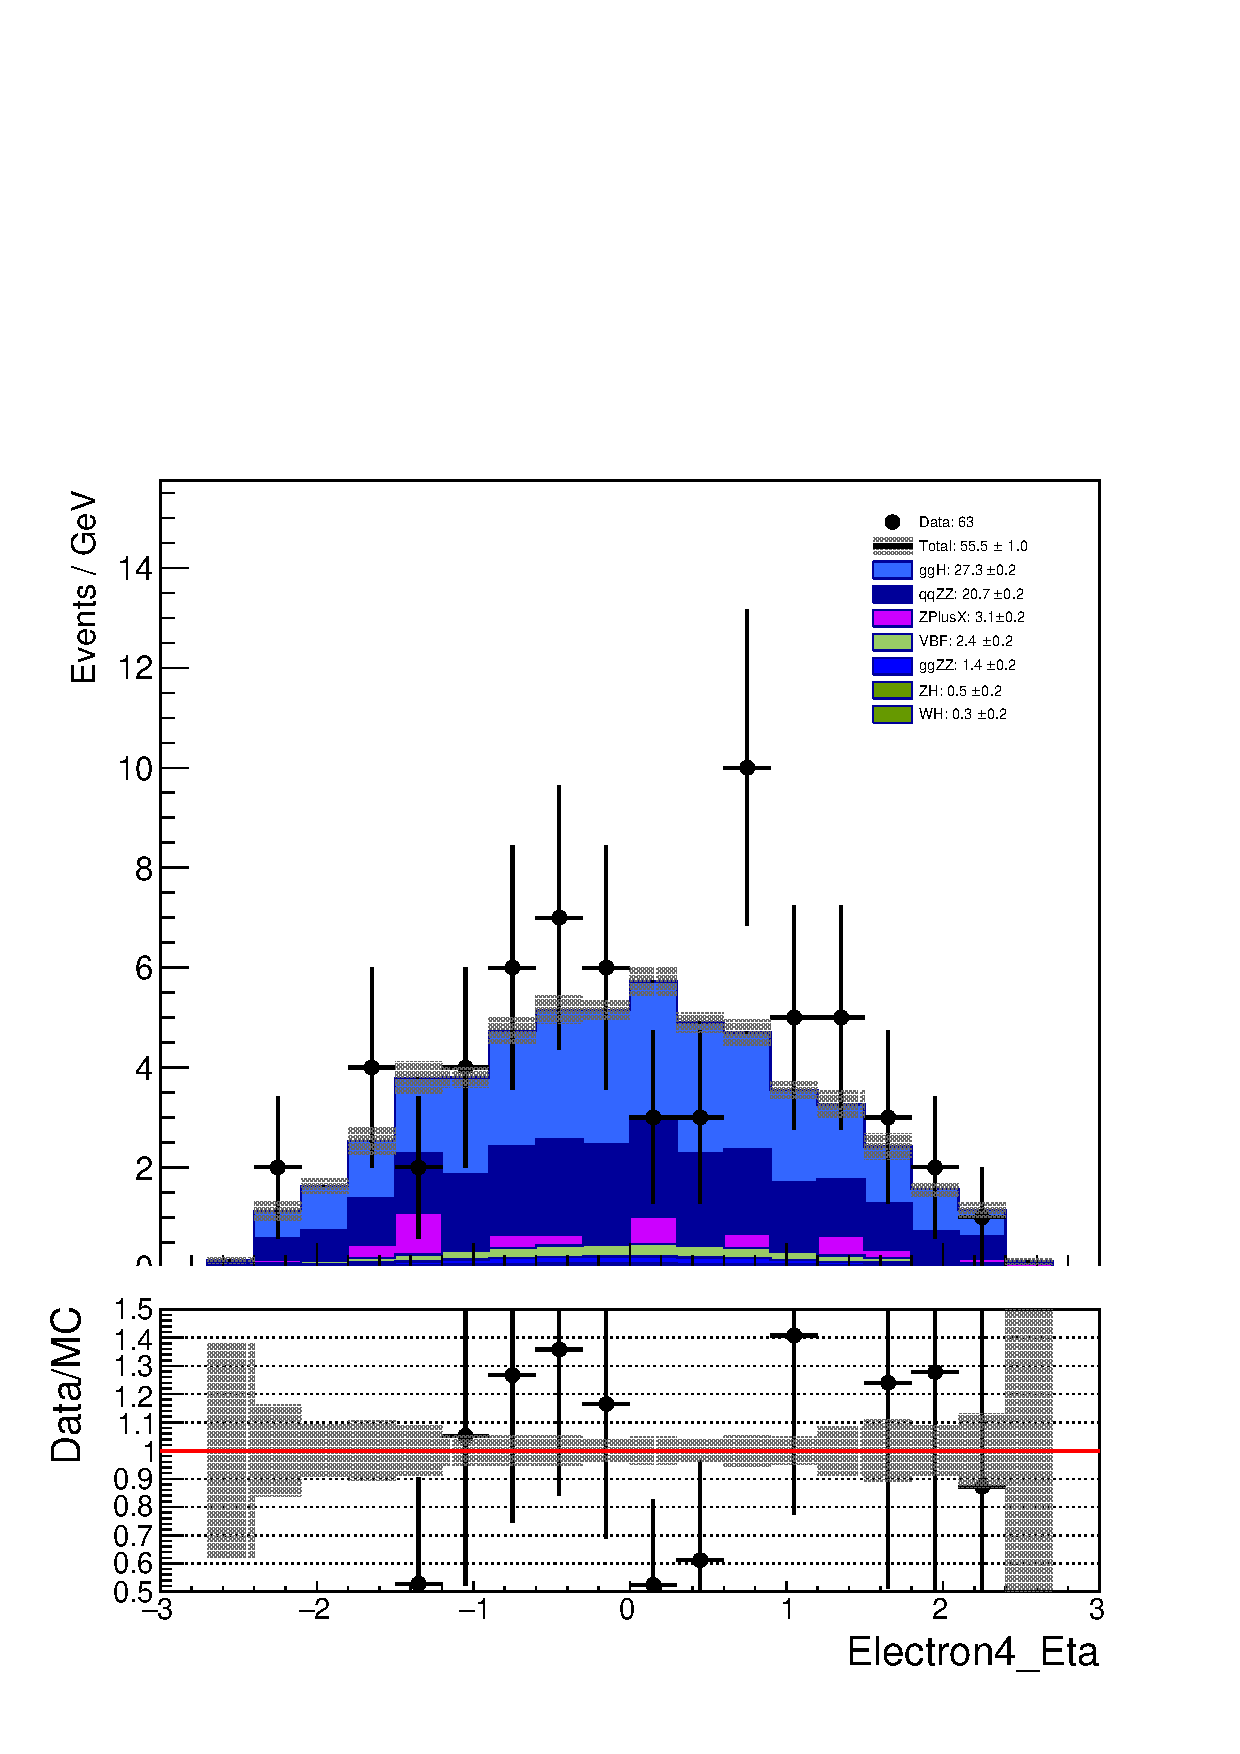
\includegraphics[width=0.49\textwidth]{Figures/Results/Distributions/DarkPhotonSR17/Electron4_Eta}}
\caption{ Distribution of the reconstructed electron~$\eta$ distribution and a comparison to predicted backgrounds using 2017 dataset.
\label{fig:eleEta_17}}
\end{figure}

%\begin{table}[h!]
%\centering
%\caption{The numbers of expected background and signal events
%and the number of observed candidate events after the full selection with $80<\mfourmu<100\GeV$.
%The signal and $\qqbar/\Pg\Pg\to4\mu$ background rates are both estimated from simulation.
%The uncertainty in the signal prediction are purely systematic uncertainties, while in the background prediction include also the
%statistical uncertainties. Also shown are the number of expected background and signal events and the number of observed
%candidate events in the relevant mass window for each $m(\cPZpr)$ hypothesis. FIXME: update table
%\label{tab:EventYieldsFull}}
%\scriptsize
%\resizebox{0.9\textwidth}{!}{
%%\begin{adjustbox}
%\setlength\extrarowheight{3pt}
%\setlength\tabcolsep{1pt}
%\renewcommand{\arraystretch}{1.1}
%\begin{tabular}{|c|c|c|c|c|c|}
% \hline
%
%\multirow{2}{*}{} & \multirow{2}{*}{Background} & $m(\Zprime)=5$\GeV & $m(\Zprime)=15$\GeV & $m(\Zprime)=70$\GeV & \multirow{2}{*}{Observed Data} \\
% & & $g_{\mu}$=0.008 & $g_{\mu}$=0.01 & $g_{\mu}$=0.5 & \\ \hline
%$80<\mfourmu<100\GeV$ & 423.0$\pm$39.2 & 37.1$\pm$3.7 & 31.4$\pm$3.1 & 53.8$\pm$5.4 & 441 \\ \hline
%$4.9<m(\cPZ_{2})<5.1\GeV$   & 9.2$\pm$3.1 & 23.3$\pm$2.3 & -- & -- & 13 \\
%$14.7<m(\cPZ_{2})<15.3\GeV$ & 7.7$\pm$2.8 & -- & 18.9$\pm$1.9 & -- & 6 \\
%$68.6<m(\cPZ_{1})<71.4\GeV$ & 34.9$\pm$6.5 & -- & -- & 36.0$\pm$3.6 & 35 \\
%\hline
%\end{tabular}
%}
%\vspace{0.5cm}
%\end{table}

\begin{figure}[!htbp]
\vspace*{0.3cm}
\centering
{ 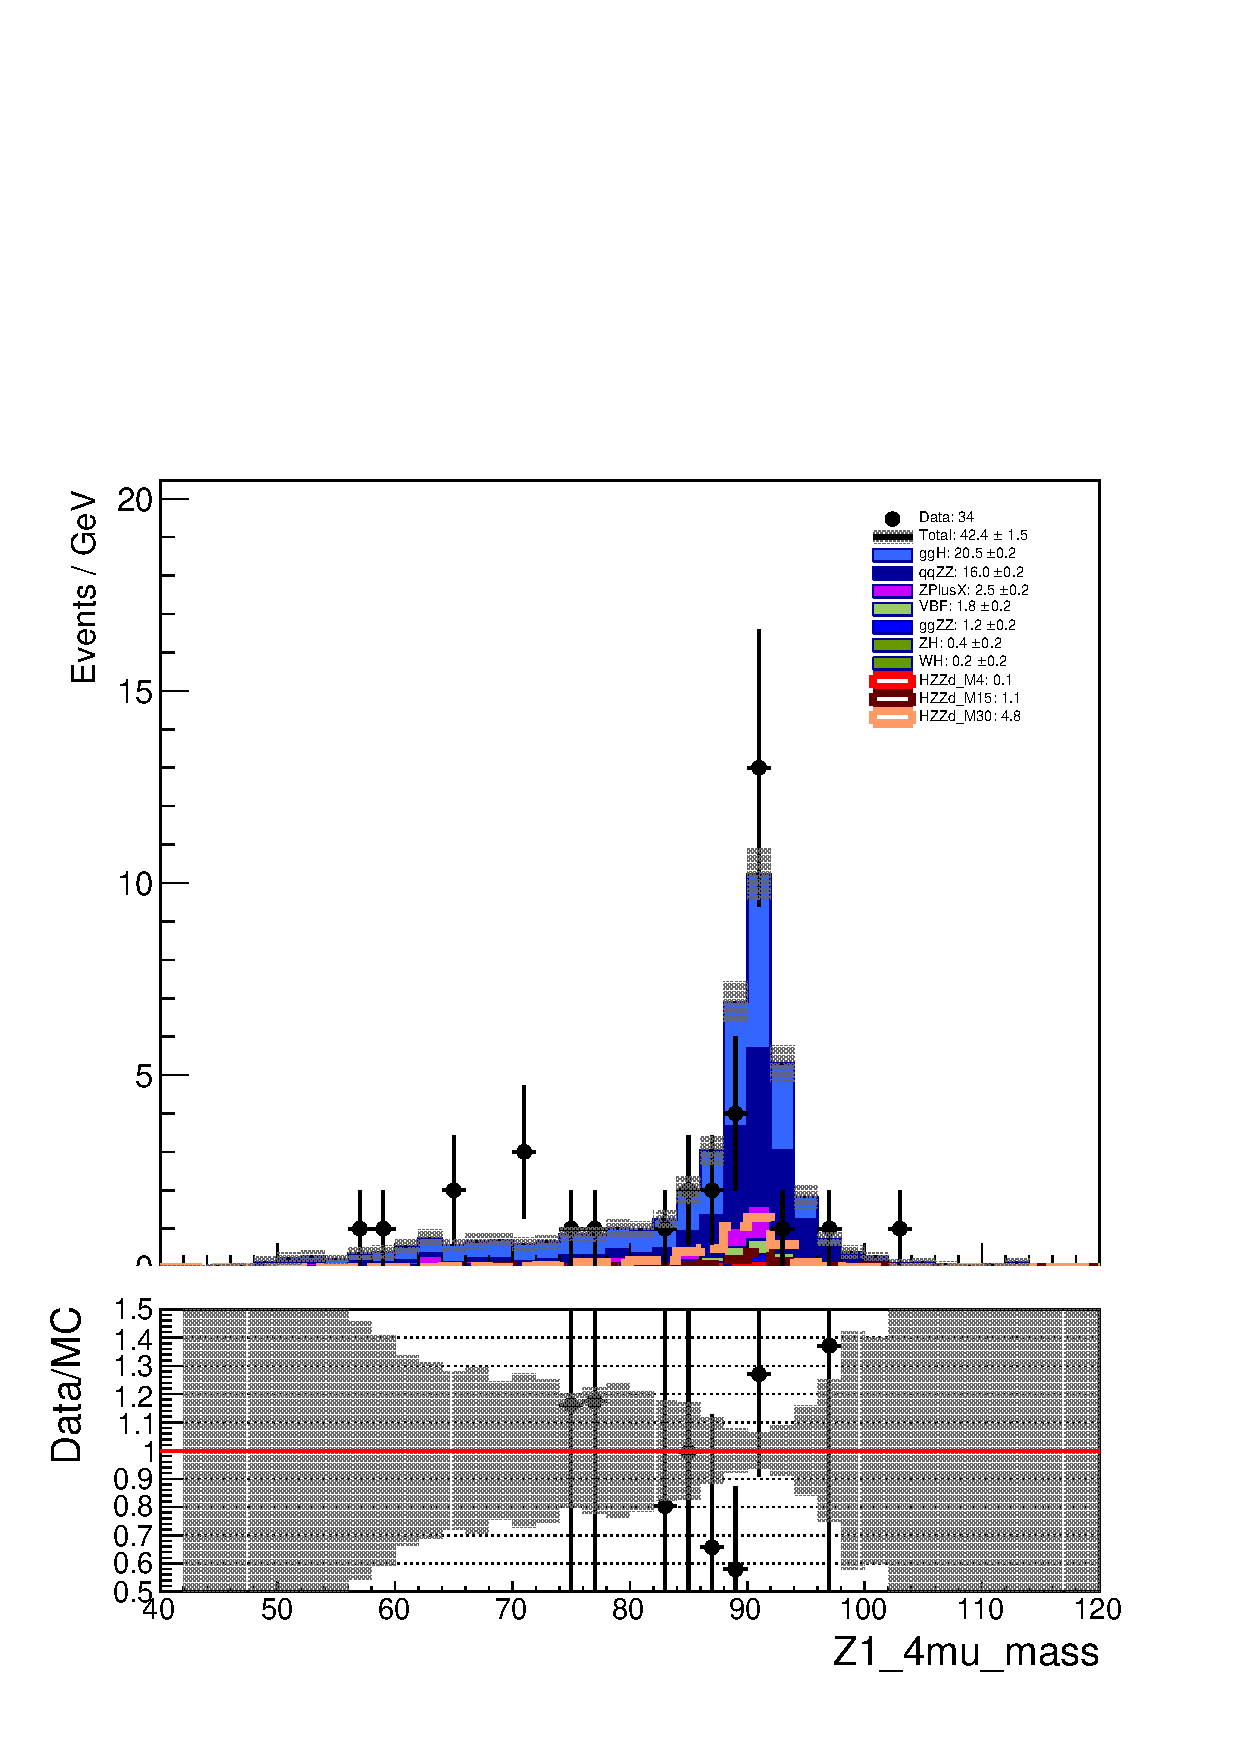
\includegraphics[width=0.45\textwidth]{Figures/Results/Distributions/DarkPhotonSR16/Z1_4mu_mass}}
{ 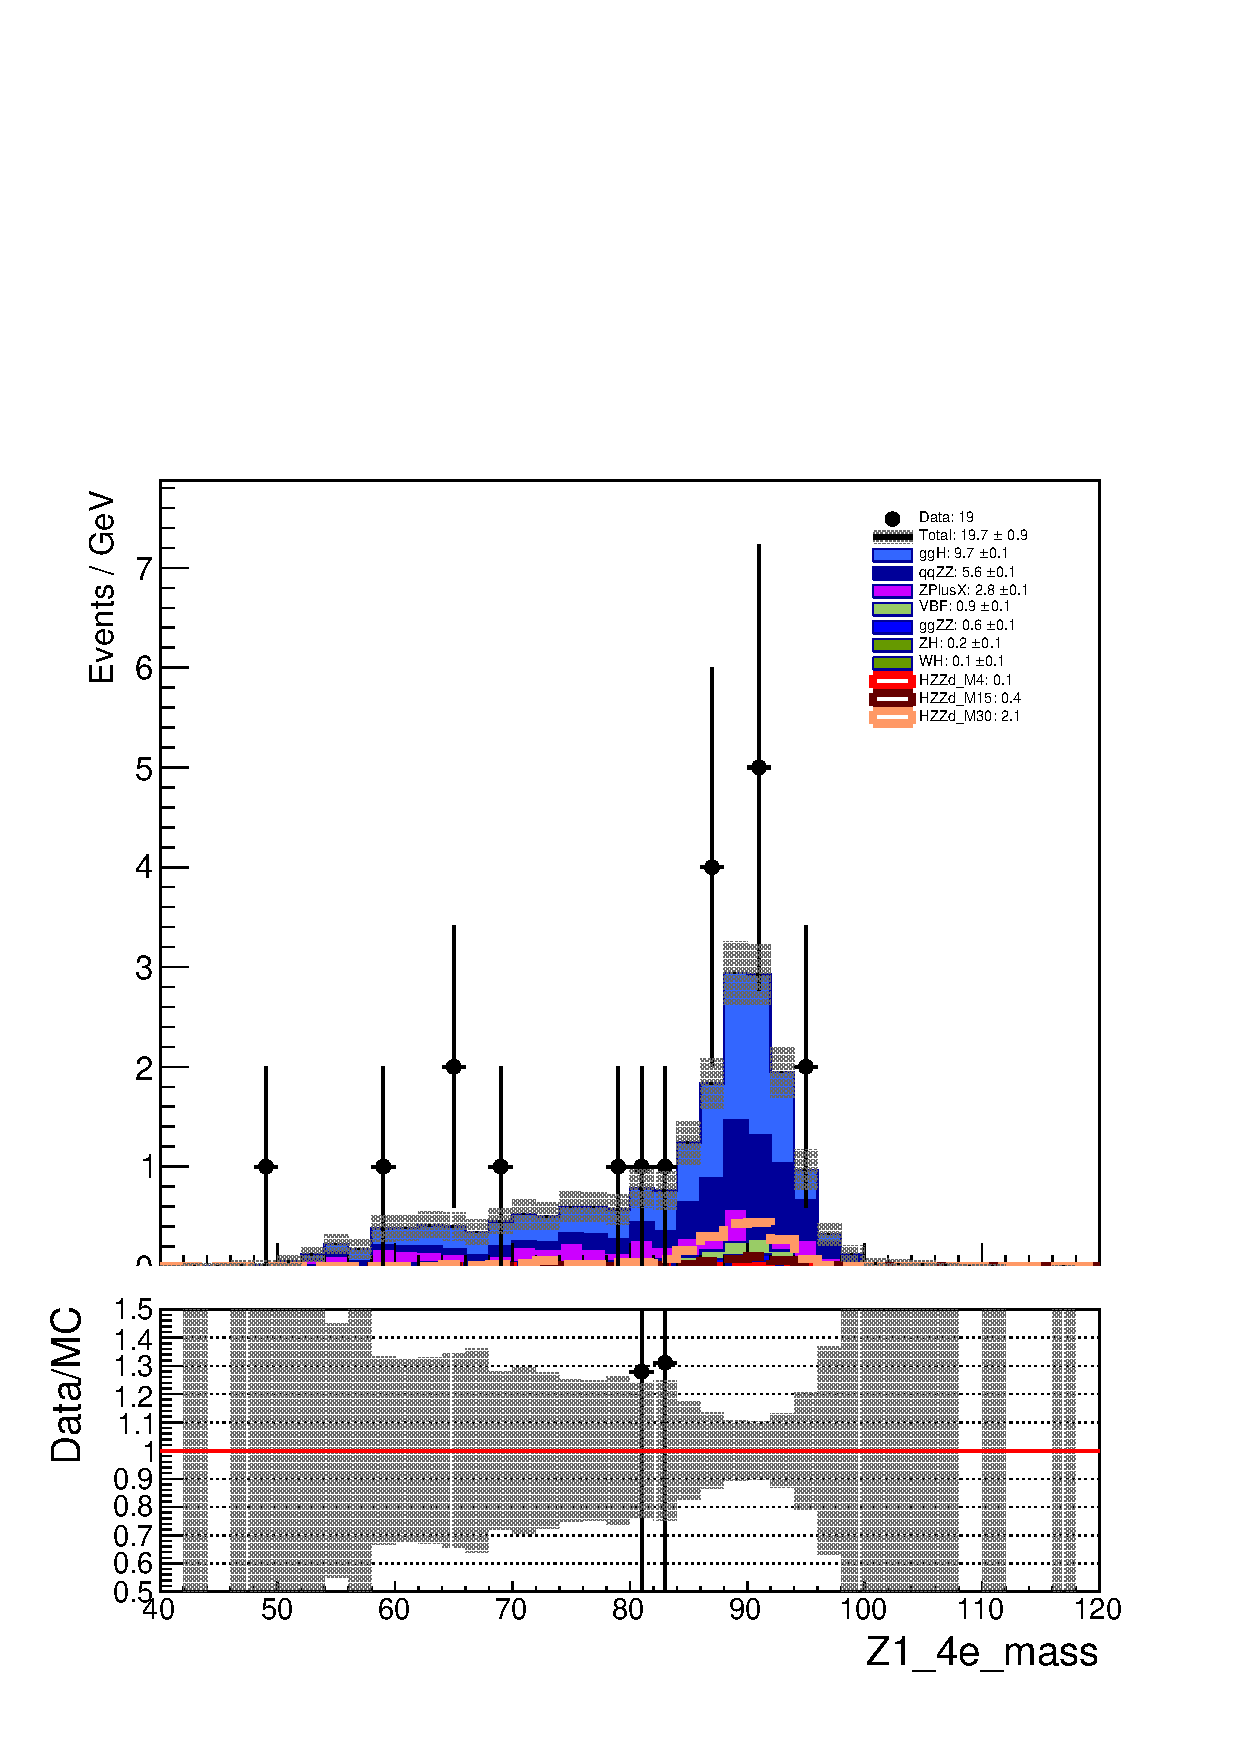
\includegraphics[width=0.45\textwidth]{Figures/Results/Distributions/DarkPhotonSR16/Z1_4e_mass}}
{ 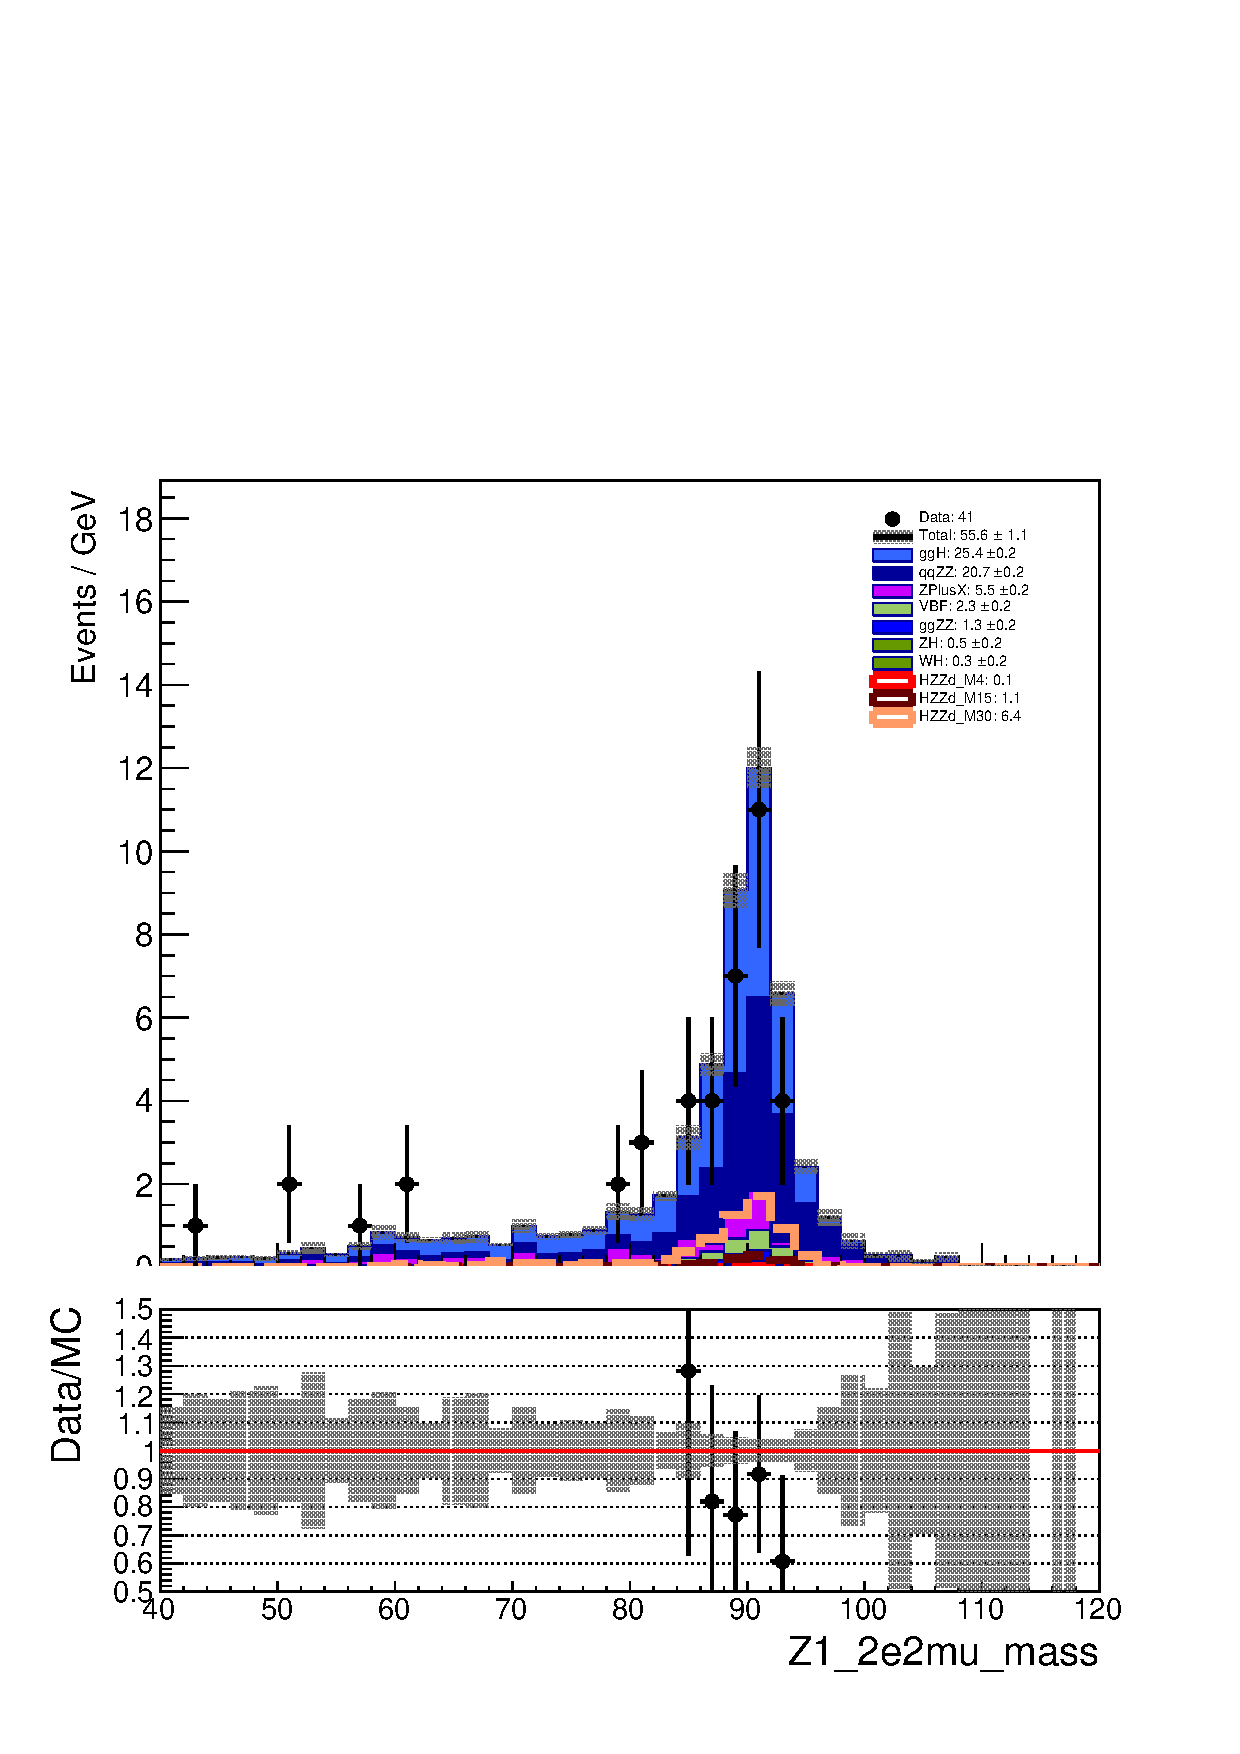
\includegraphics[width=0.45\textwidth]{Figures/Results/Distributions/DarkPhotonSR16/Z1_2e2mu_mass}}
{ \includegraphics[width=0.45\textwidth]{Figures/Results/Distributions/DarkPhotonSR16/Z1_2mu2e_mass}}
\caption{Distributions of the reconstructed \mass{Z1} and a comparison to predicted backgrounds using 2016 dataset. Different \zd signal hypothesis are also shown.
\label{fig:massZ1_16}}
\end{figure}

\begin{figure}[!htbp]
\vspace*{0.3cm}
\centering
{ 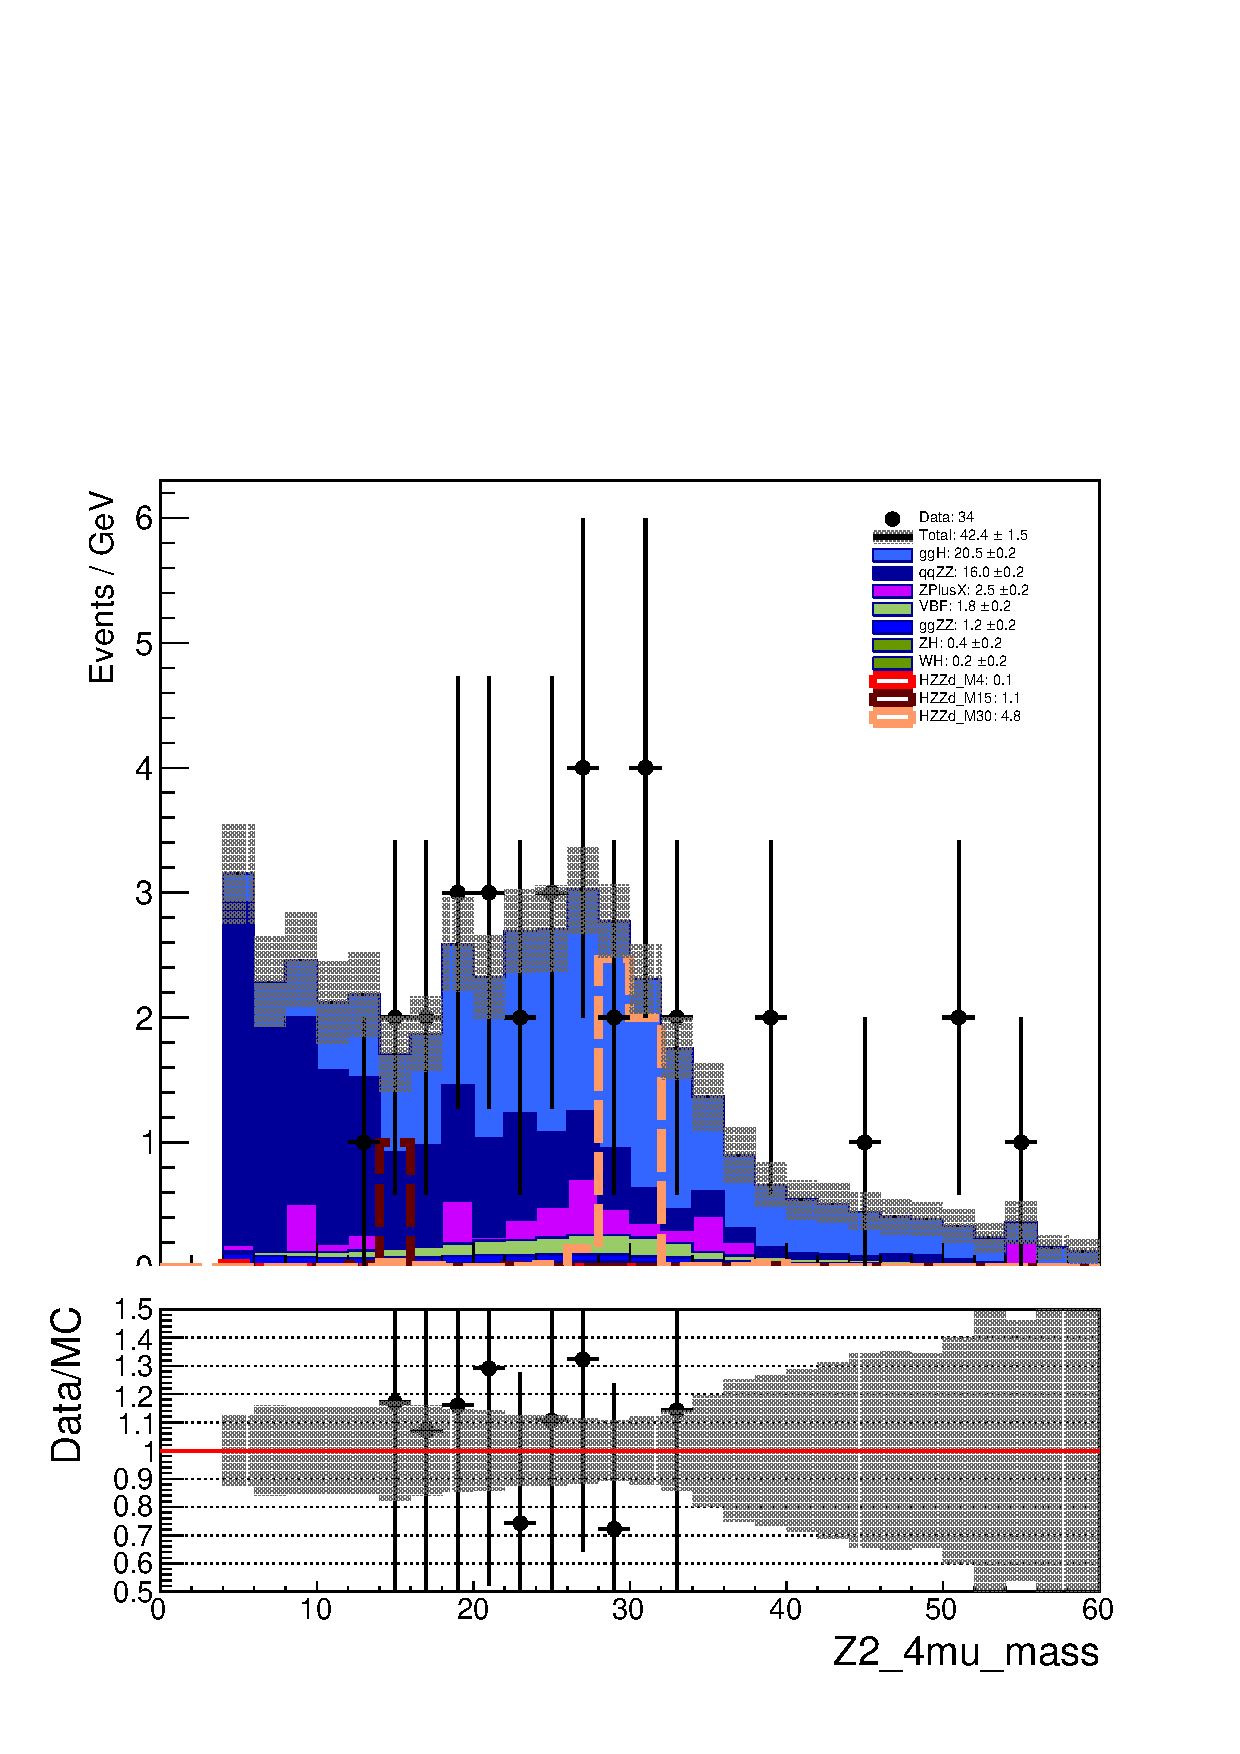
\includegraphics[width=0.45\textwidth]{Figures/Results/Distributions/DarkPhotonSR16/Z2_4mu_mass}}
{ 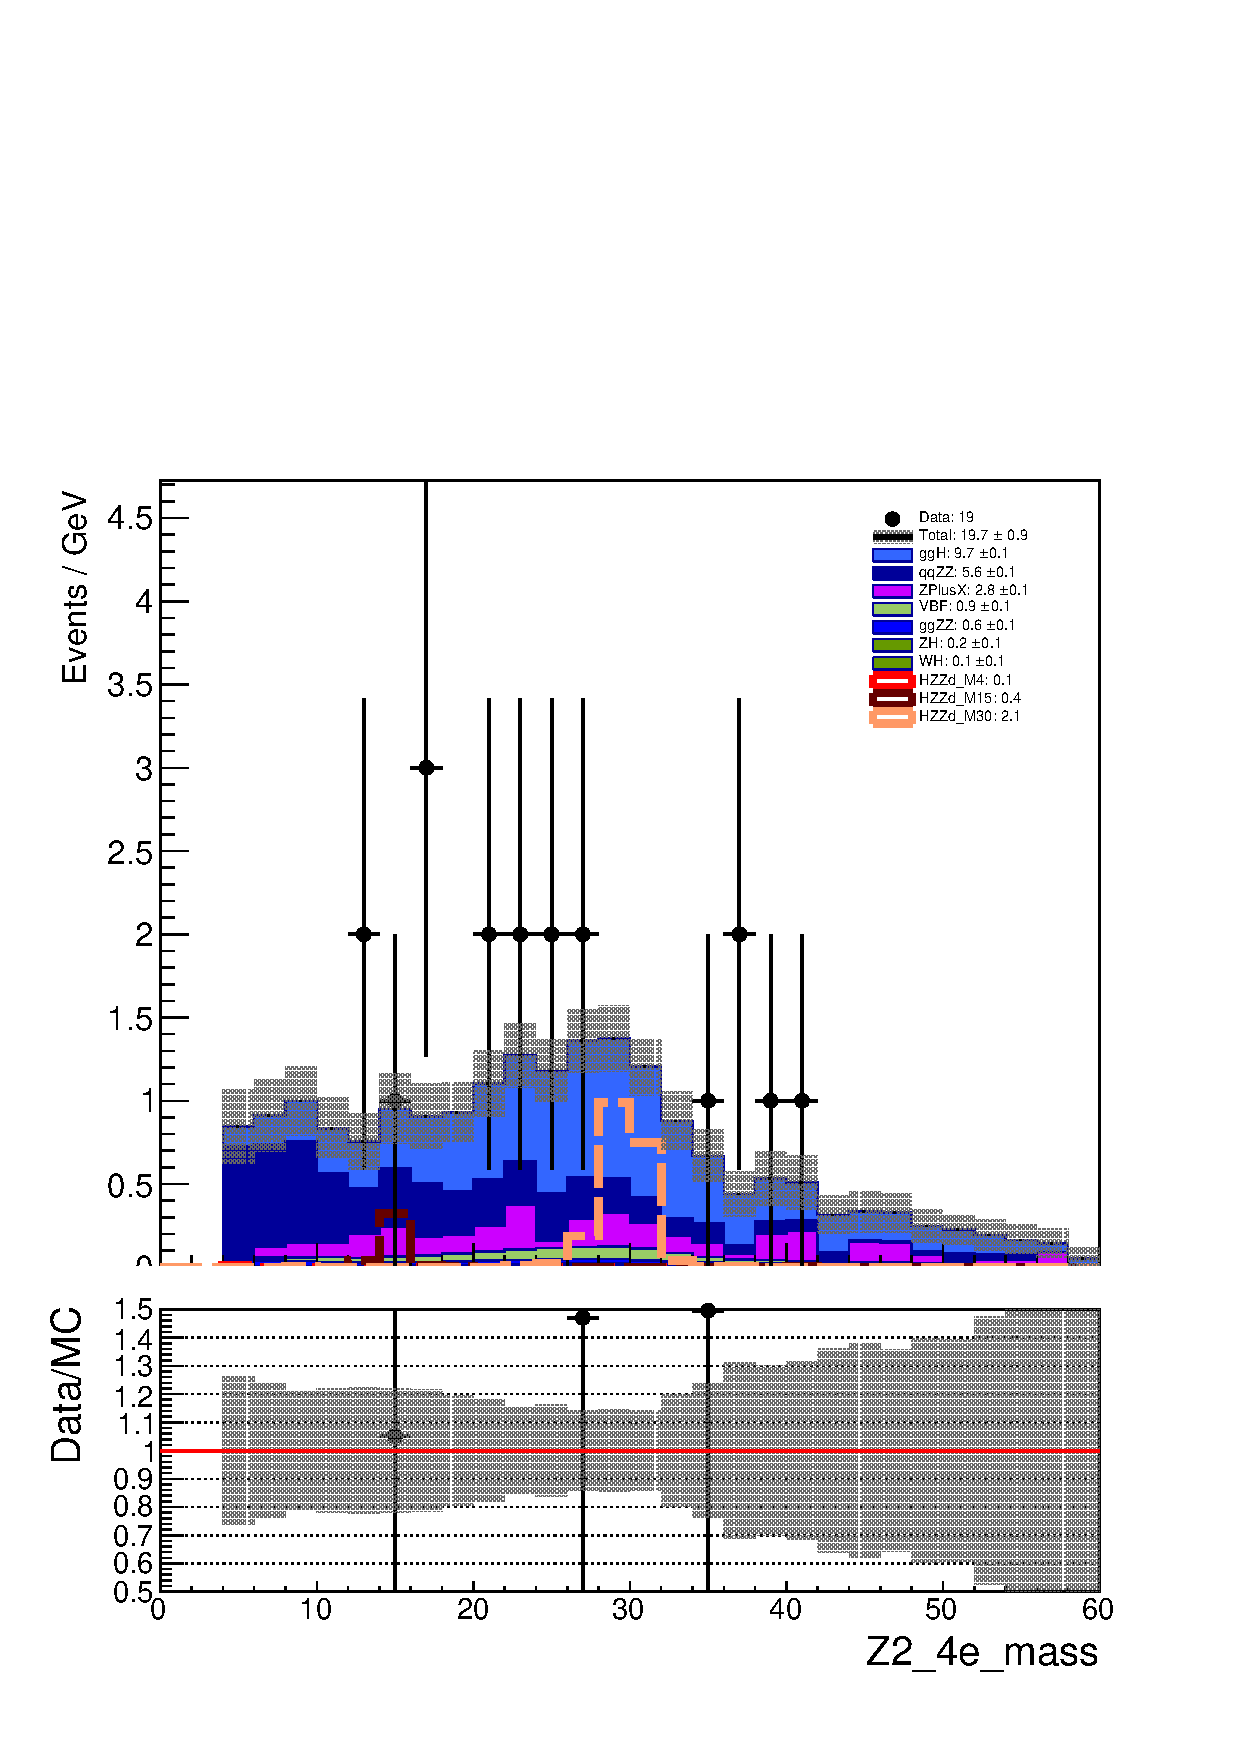
\includegraphics[width=0.45\textwidth]{Figures/Results/Distributions/DarkPhotonSR16/Z2_4e_mass}}
{ 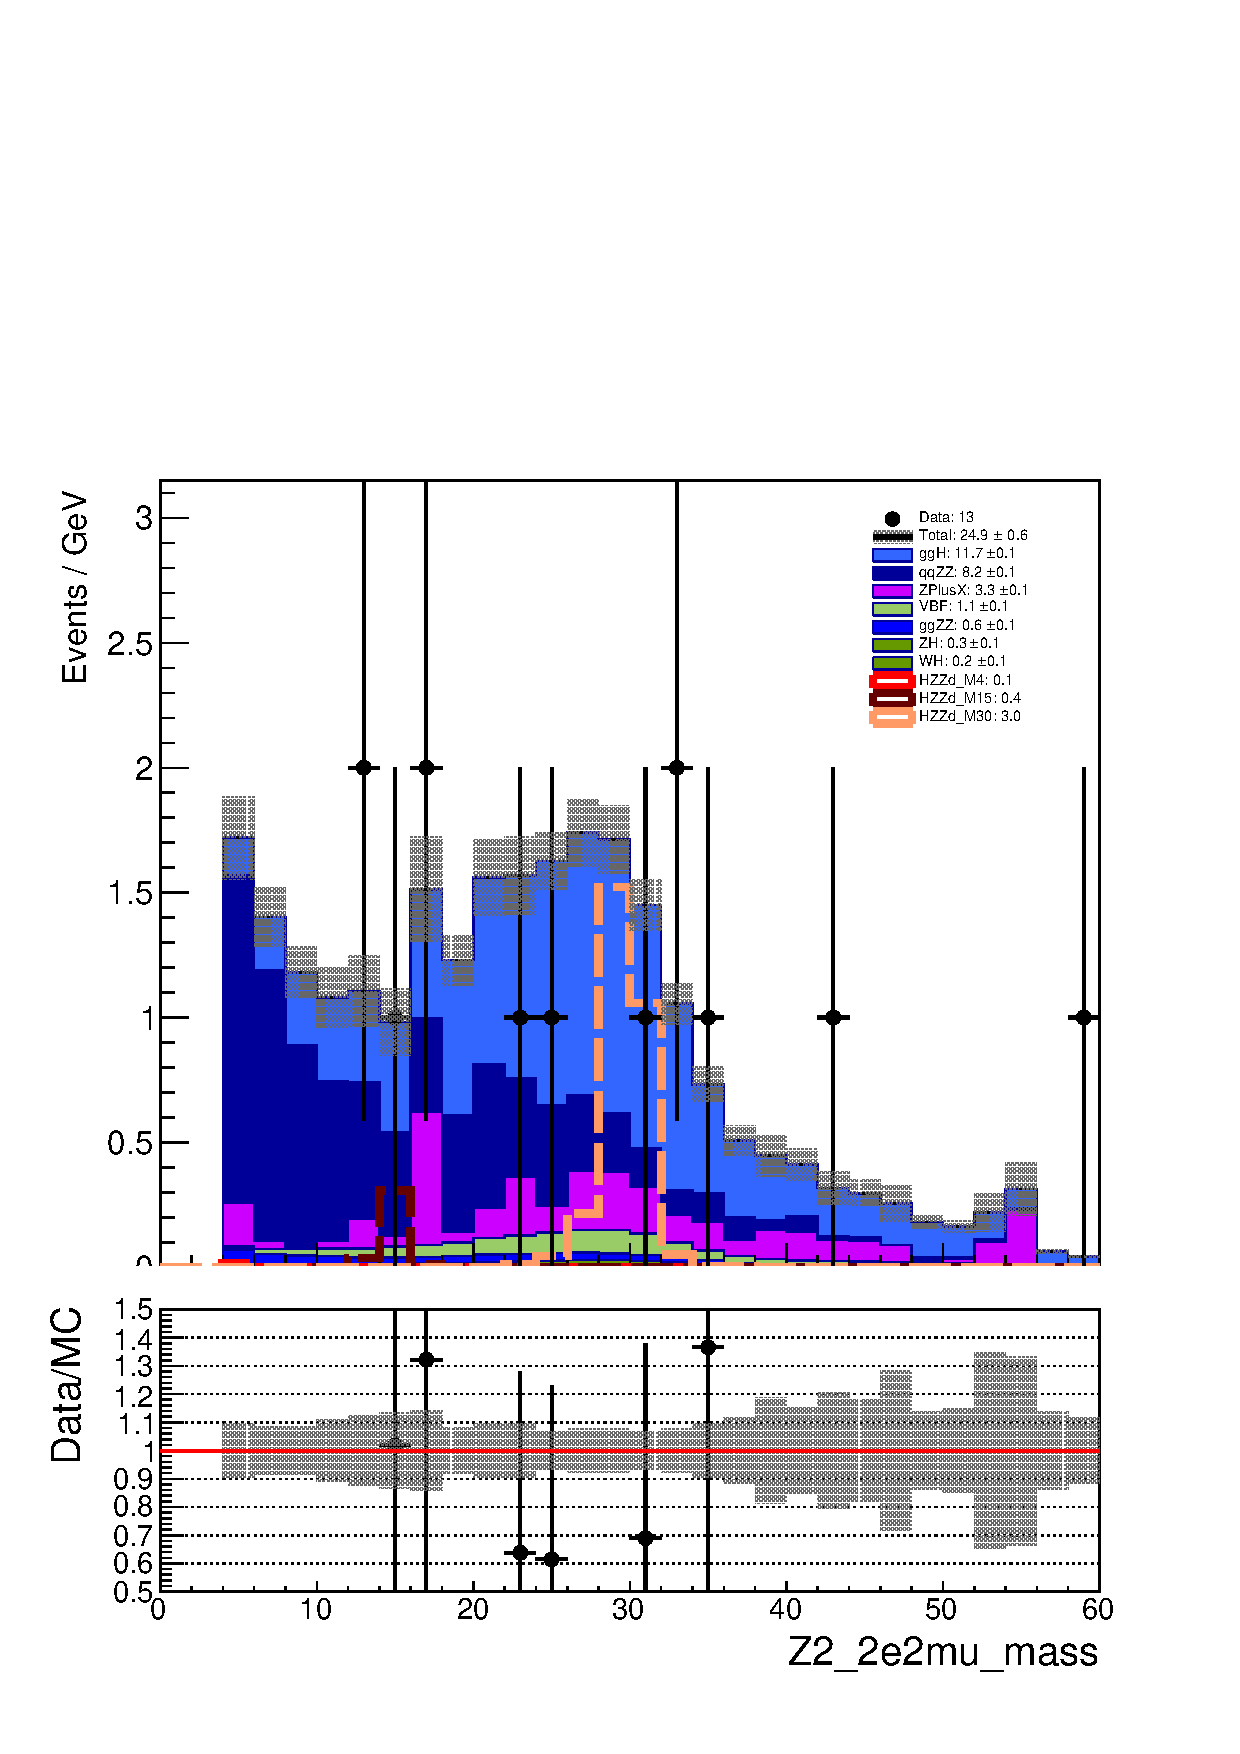
\includegraphics[width=0.45\textwidth]{Figures/Results/Distributions/DarkPhotonSR16/Z2_2e2mu_mass}}
{ 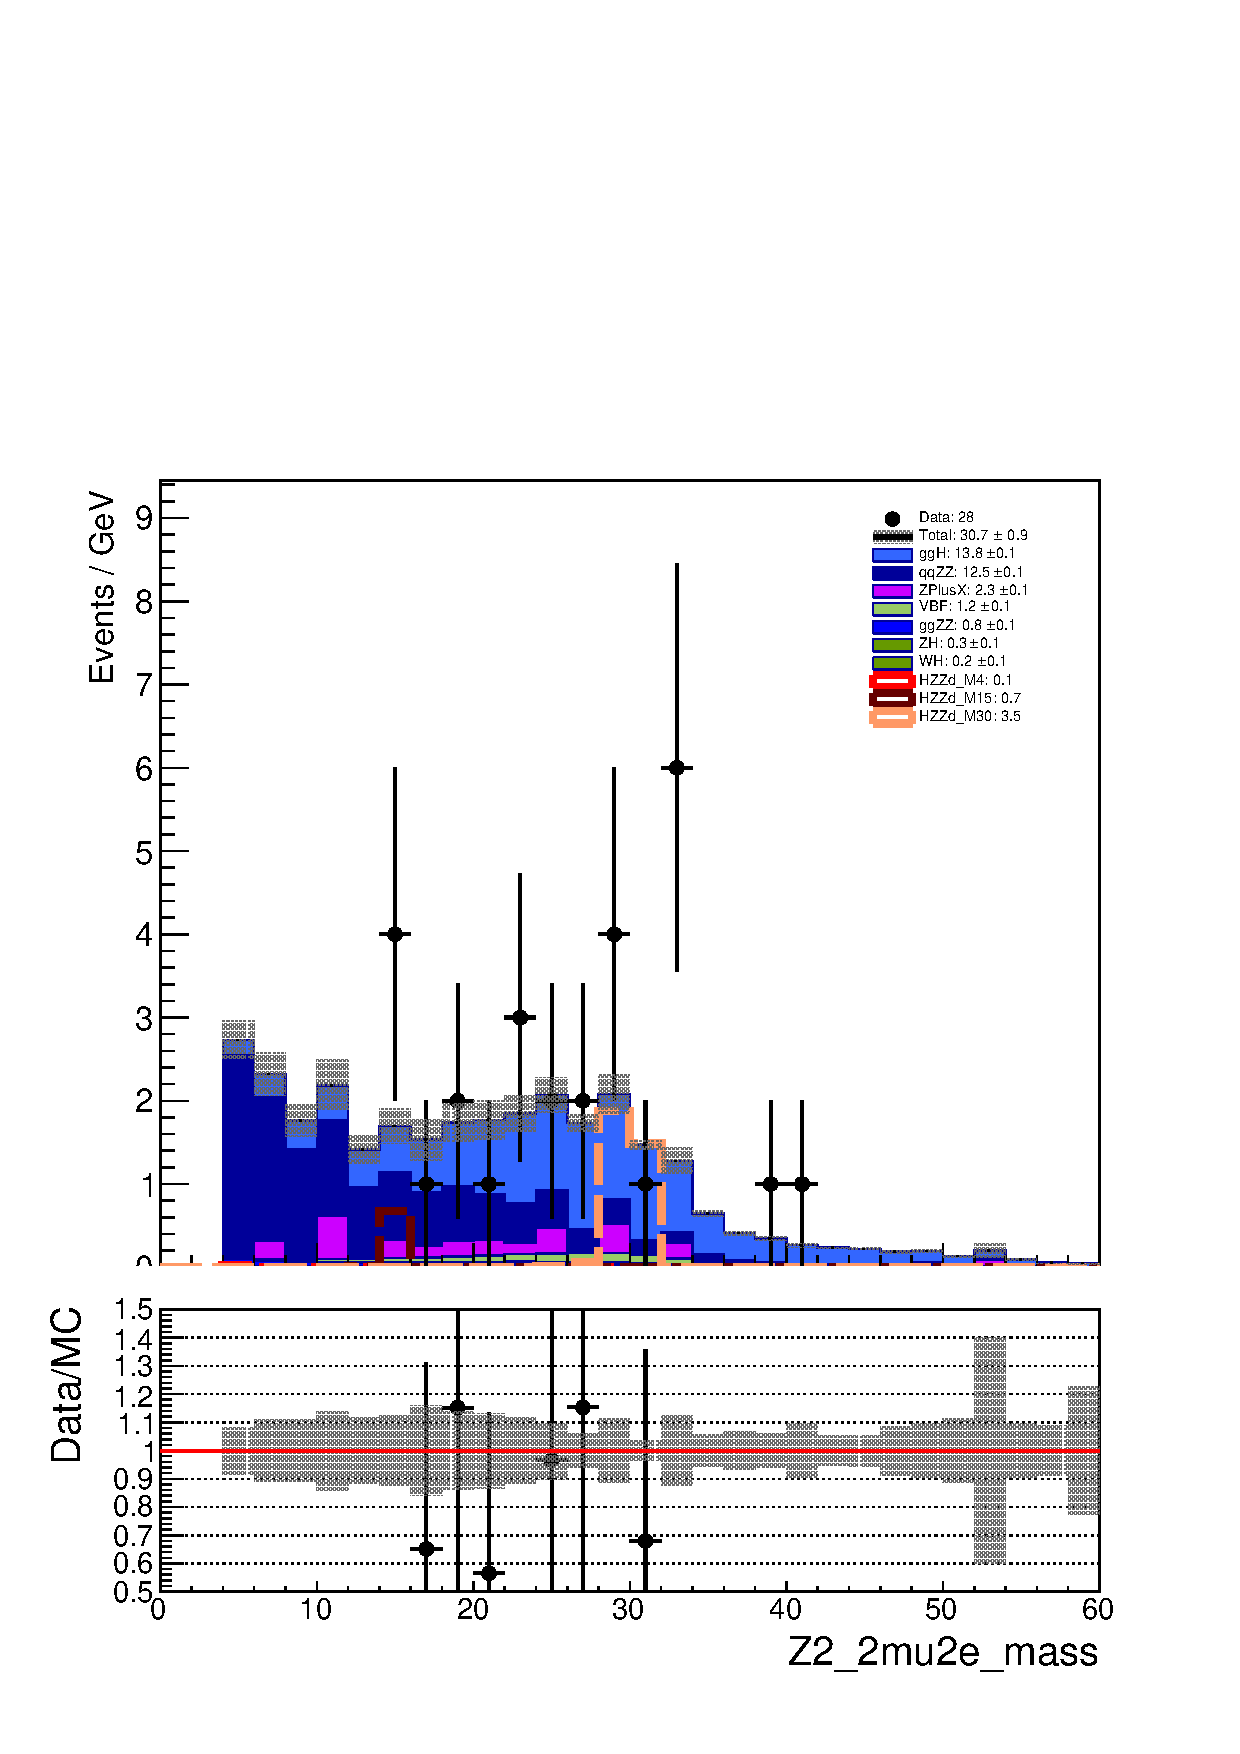
\includegraphics[width=0.45\textwidth]{Figures/Results/Distributions/DarkPhotonSR16/Z2_2mu2e_mass}}
\caption{Distributions of the reconstructed \mass{Z2} and a comparison to predicted backgrounds using 2016 dataset. Different \zd signal hypothesis are also shown.
\label{fig:massZ2_16}}
\end{figure}

\begin{figure}[!htbp]
\vspace*{0.3cm}
\centering
{ 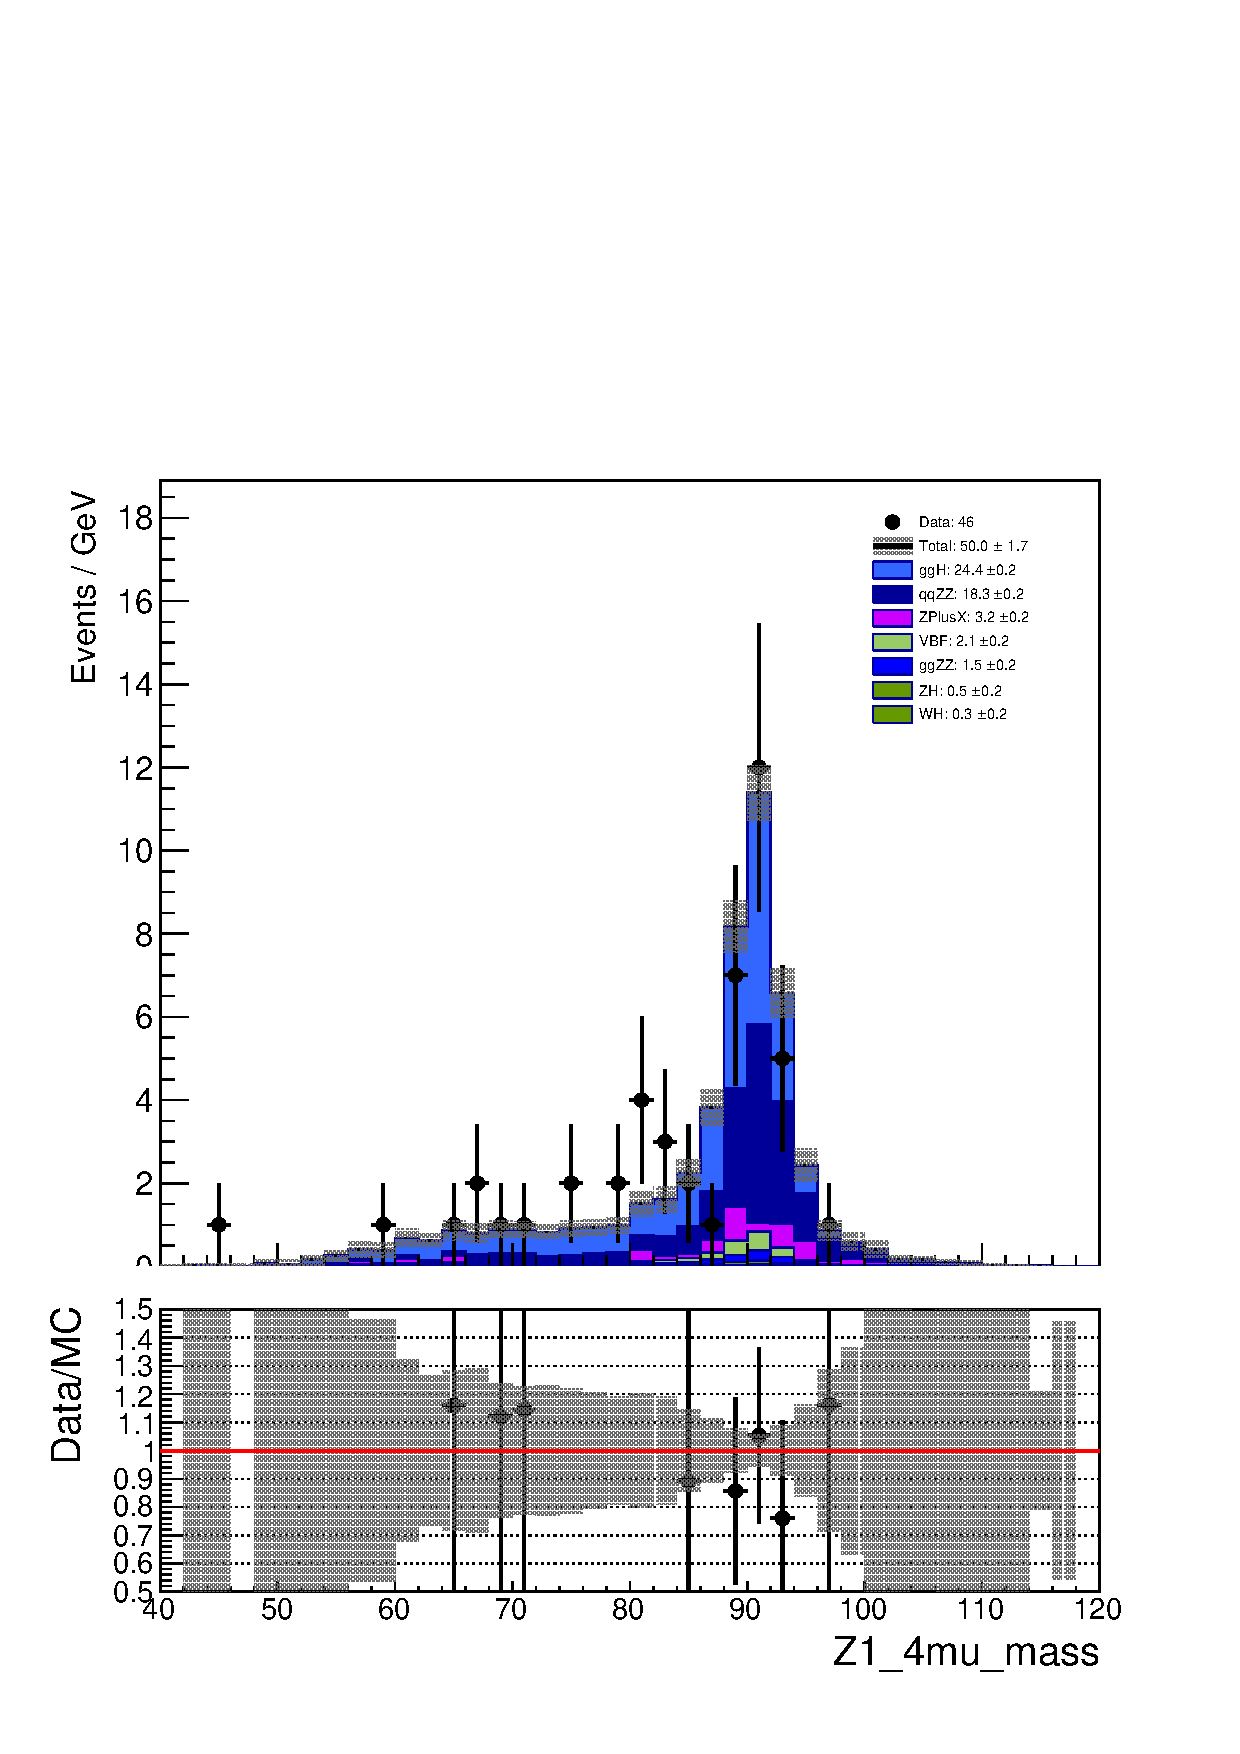
\includegraphics[width=0.45\textwidth]{Figures/Results/Distributions/DarkPhotonSR17/Z1_4mu_mass}}
{ 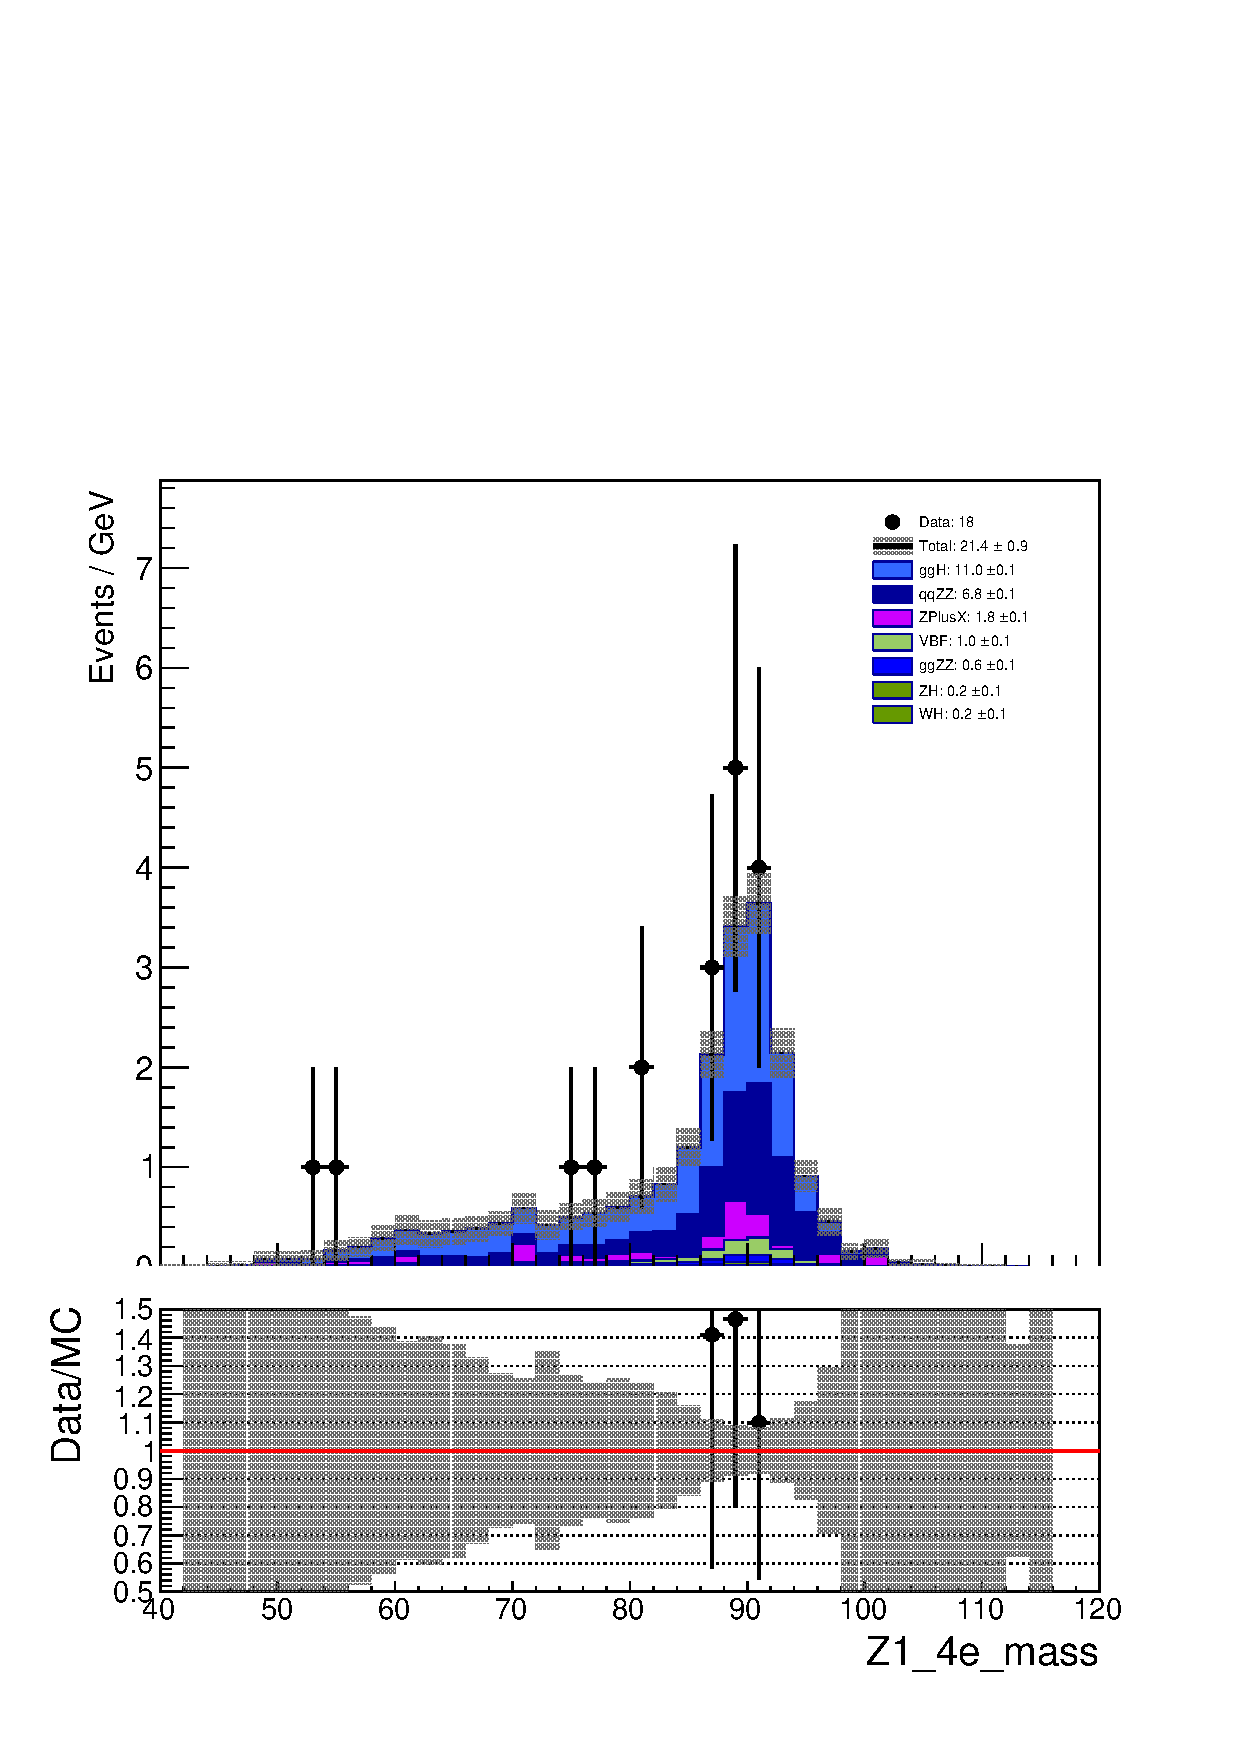
\includegraphics[width=0.45\textwidth]{Figures/Results/Distributions/DarkPhotonSR17/Z1_4e_mass}}
{ 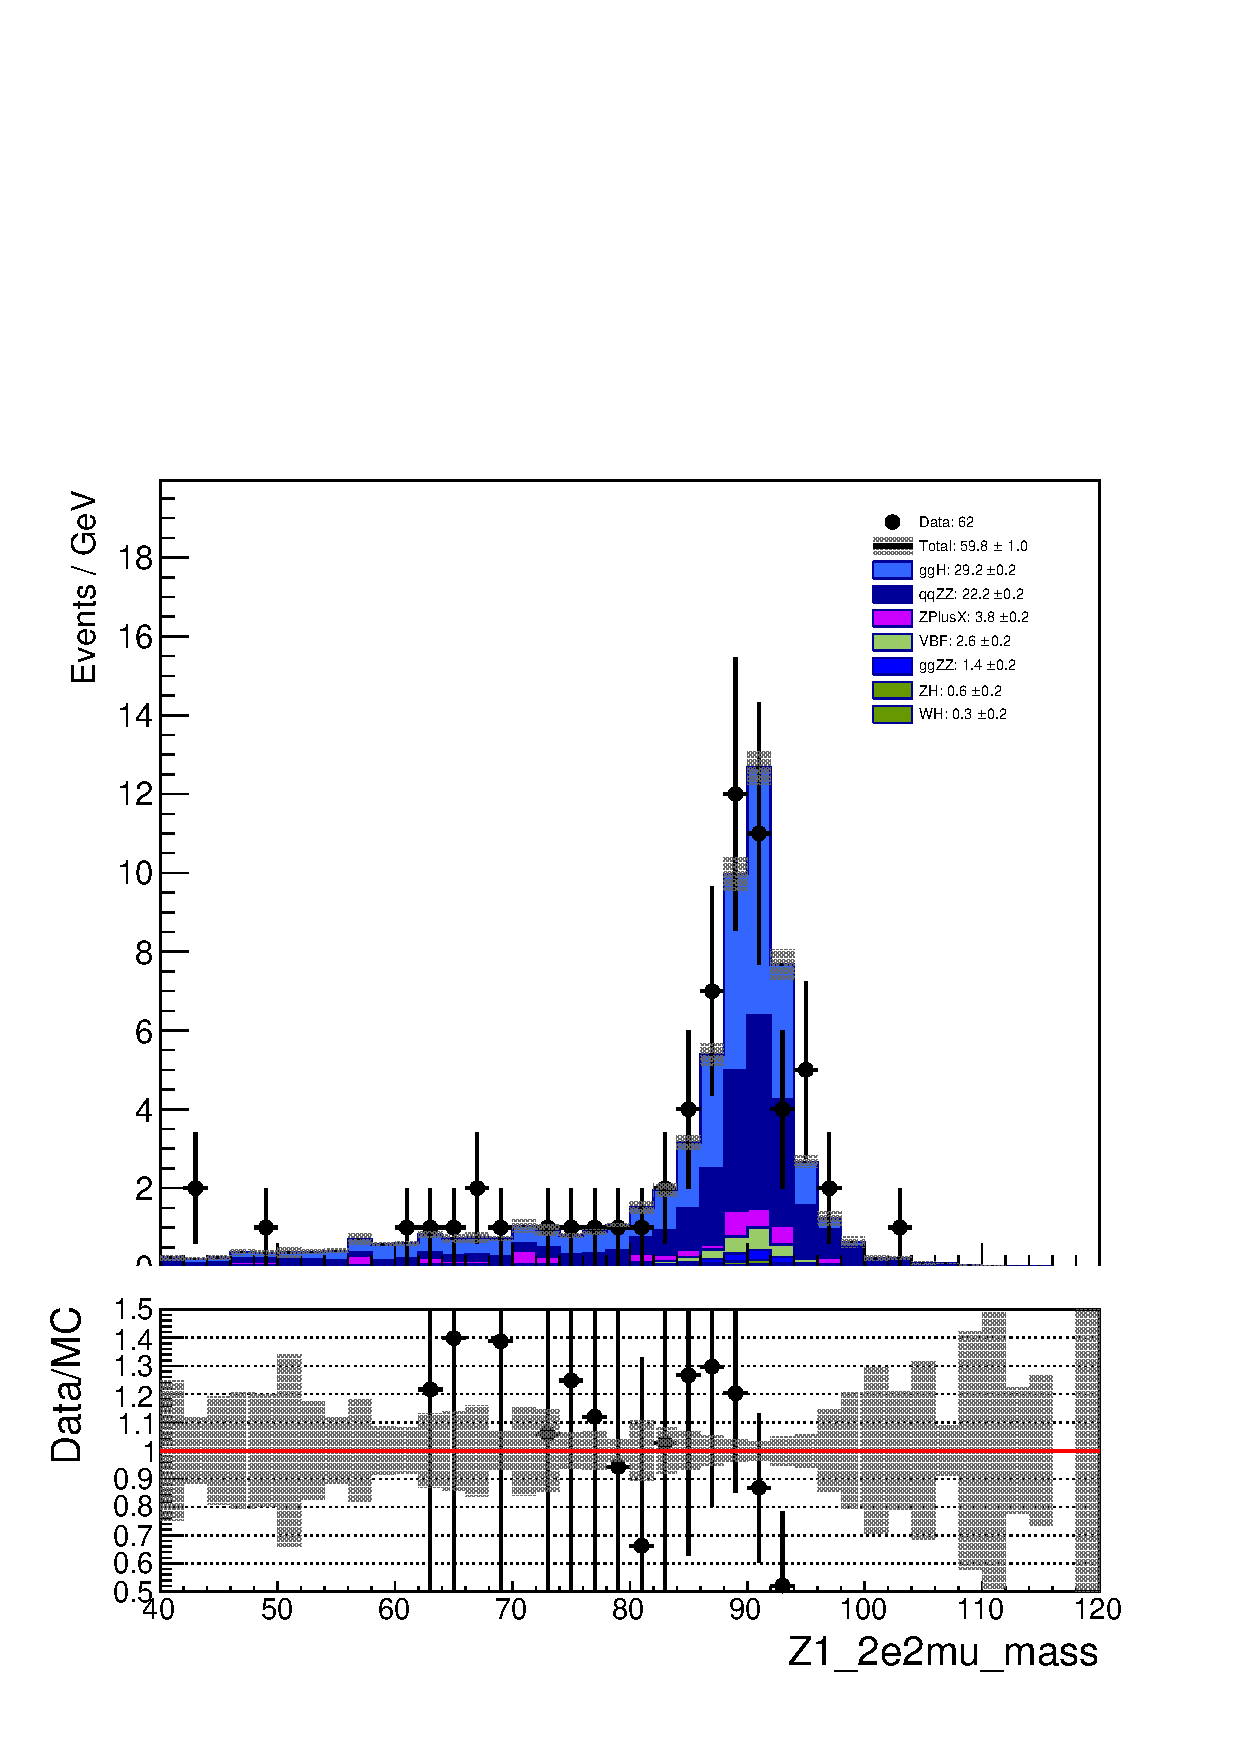
\includegraphics[width=0.45\textwidth]{Figures/Results/Distributions/DarkPhotonSR17/Z1_2e2mu_mass}}
{ \includegraphics[width=0.45\textwidth]{Figures/Results/Distributions/DarkPhotonSR17/Z1_2mu2e_mass}}
\caption{Distributions of the reconstructed \mass{Z1} and a comparison to predicted backgrounds using 2017 dataset. Different \zd signal hypothesis are also shown.
\label{fig:massZ1_17}}
\end{figure}

\begin{figure}[!htbp]
\vspace*{0.3cm}
\centering
{ 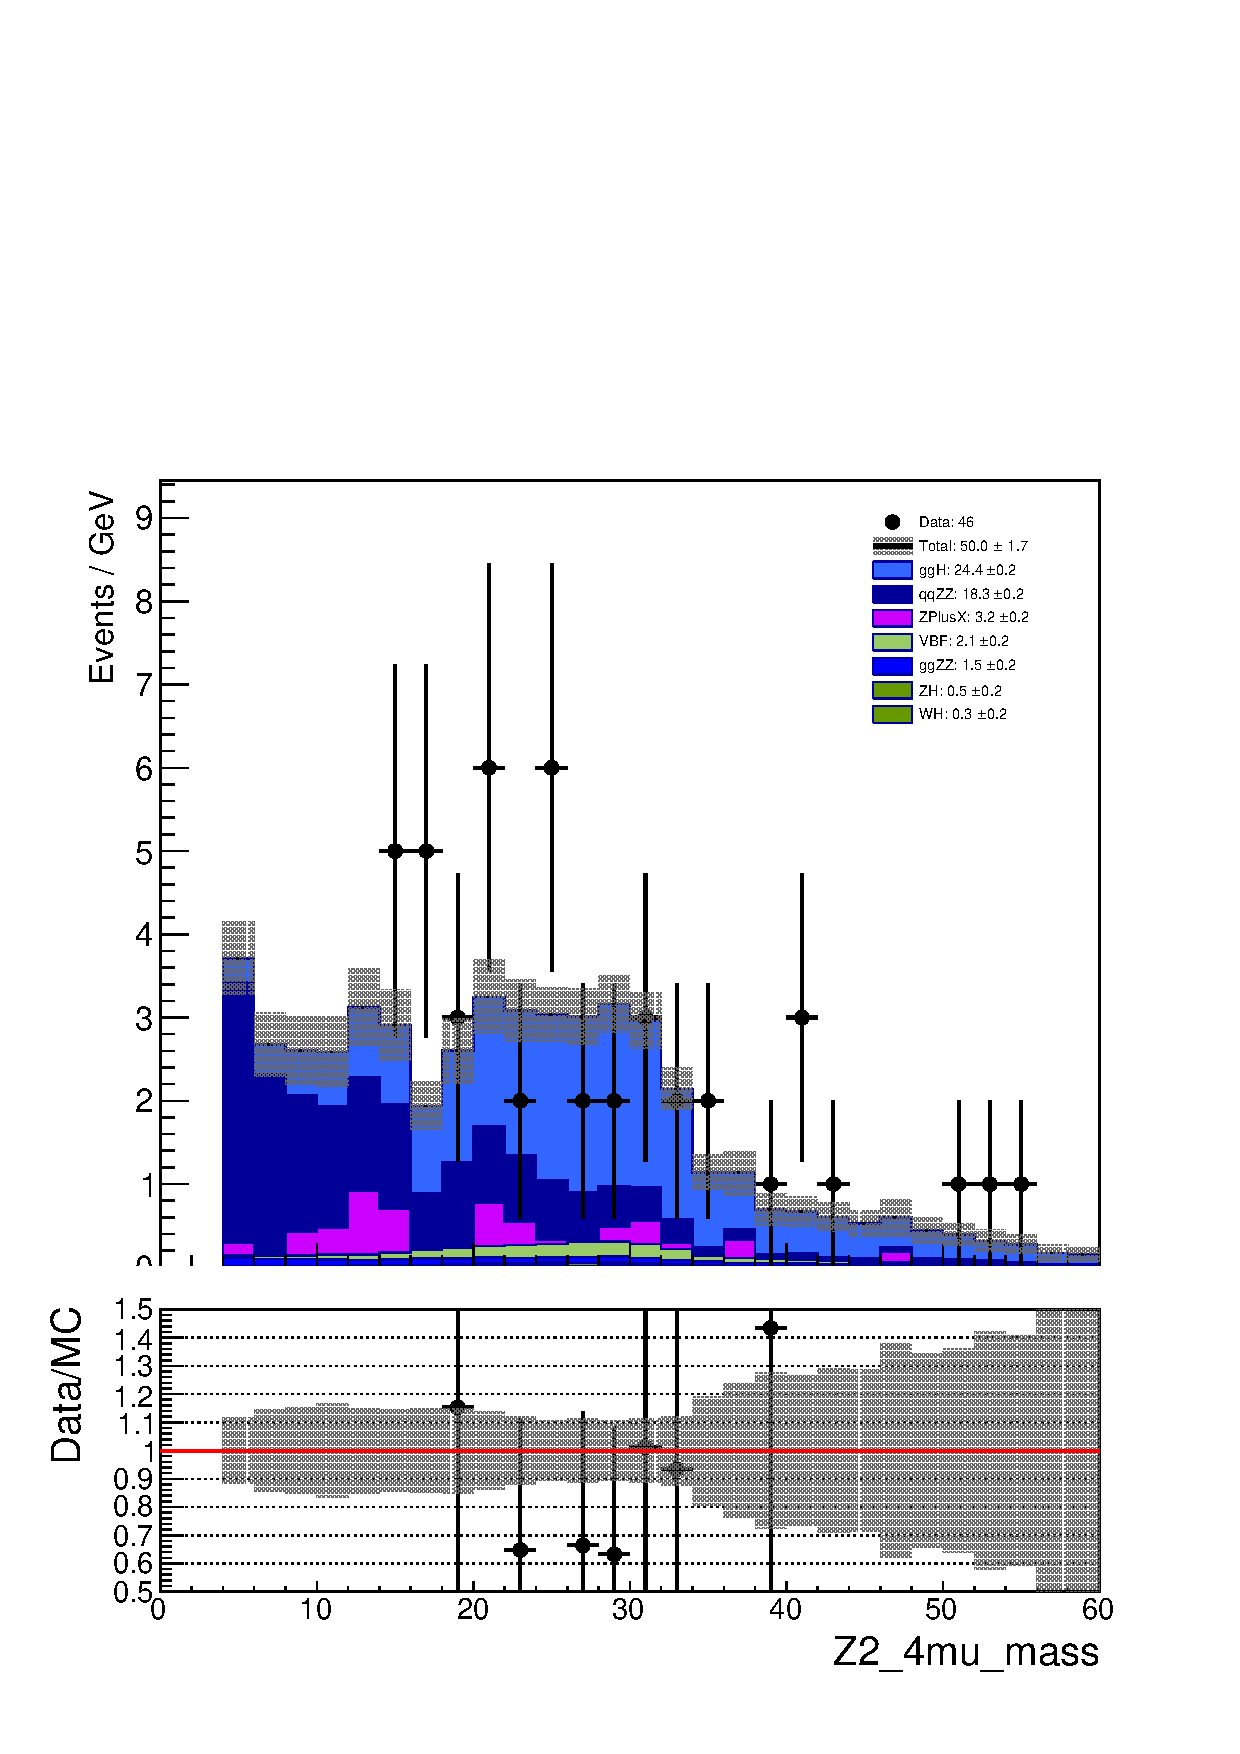
\includegraphics[width=0.45\textwidth]{Figures/Results/Distributions/DarkPhotonSR17/Z2_4mu_mass}}
{ 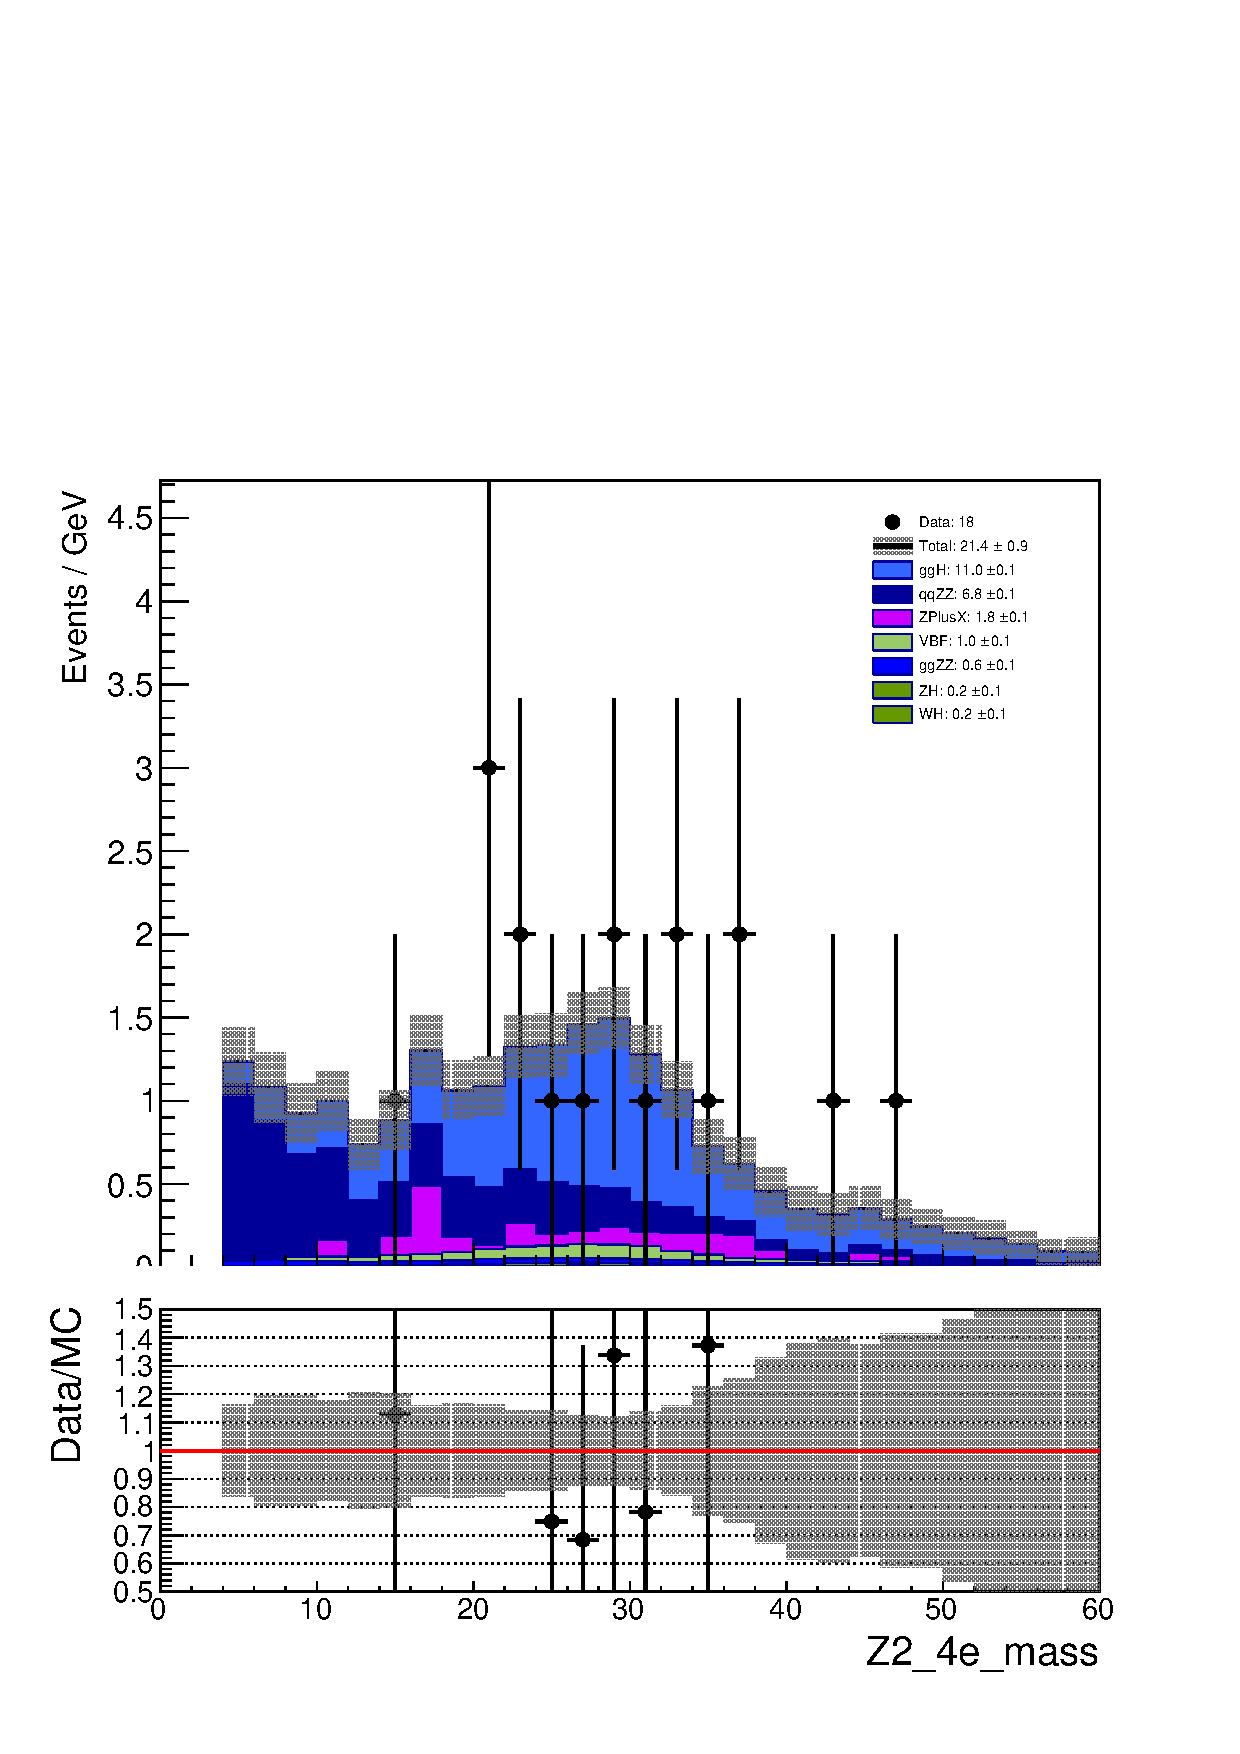
\includegraphics[width=0.45\textwidth]{Figures/Results/Distributions/DarkPhotonSR17/Z2_4e_mass}}
{ 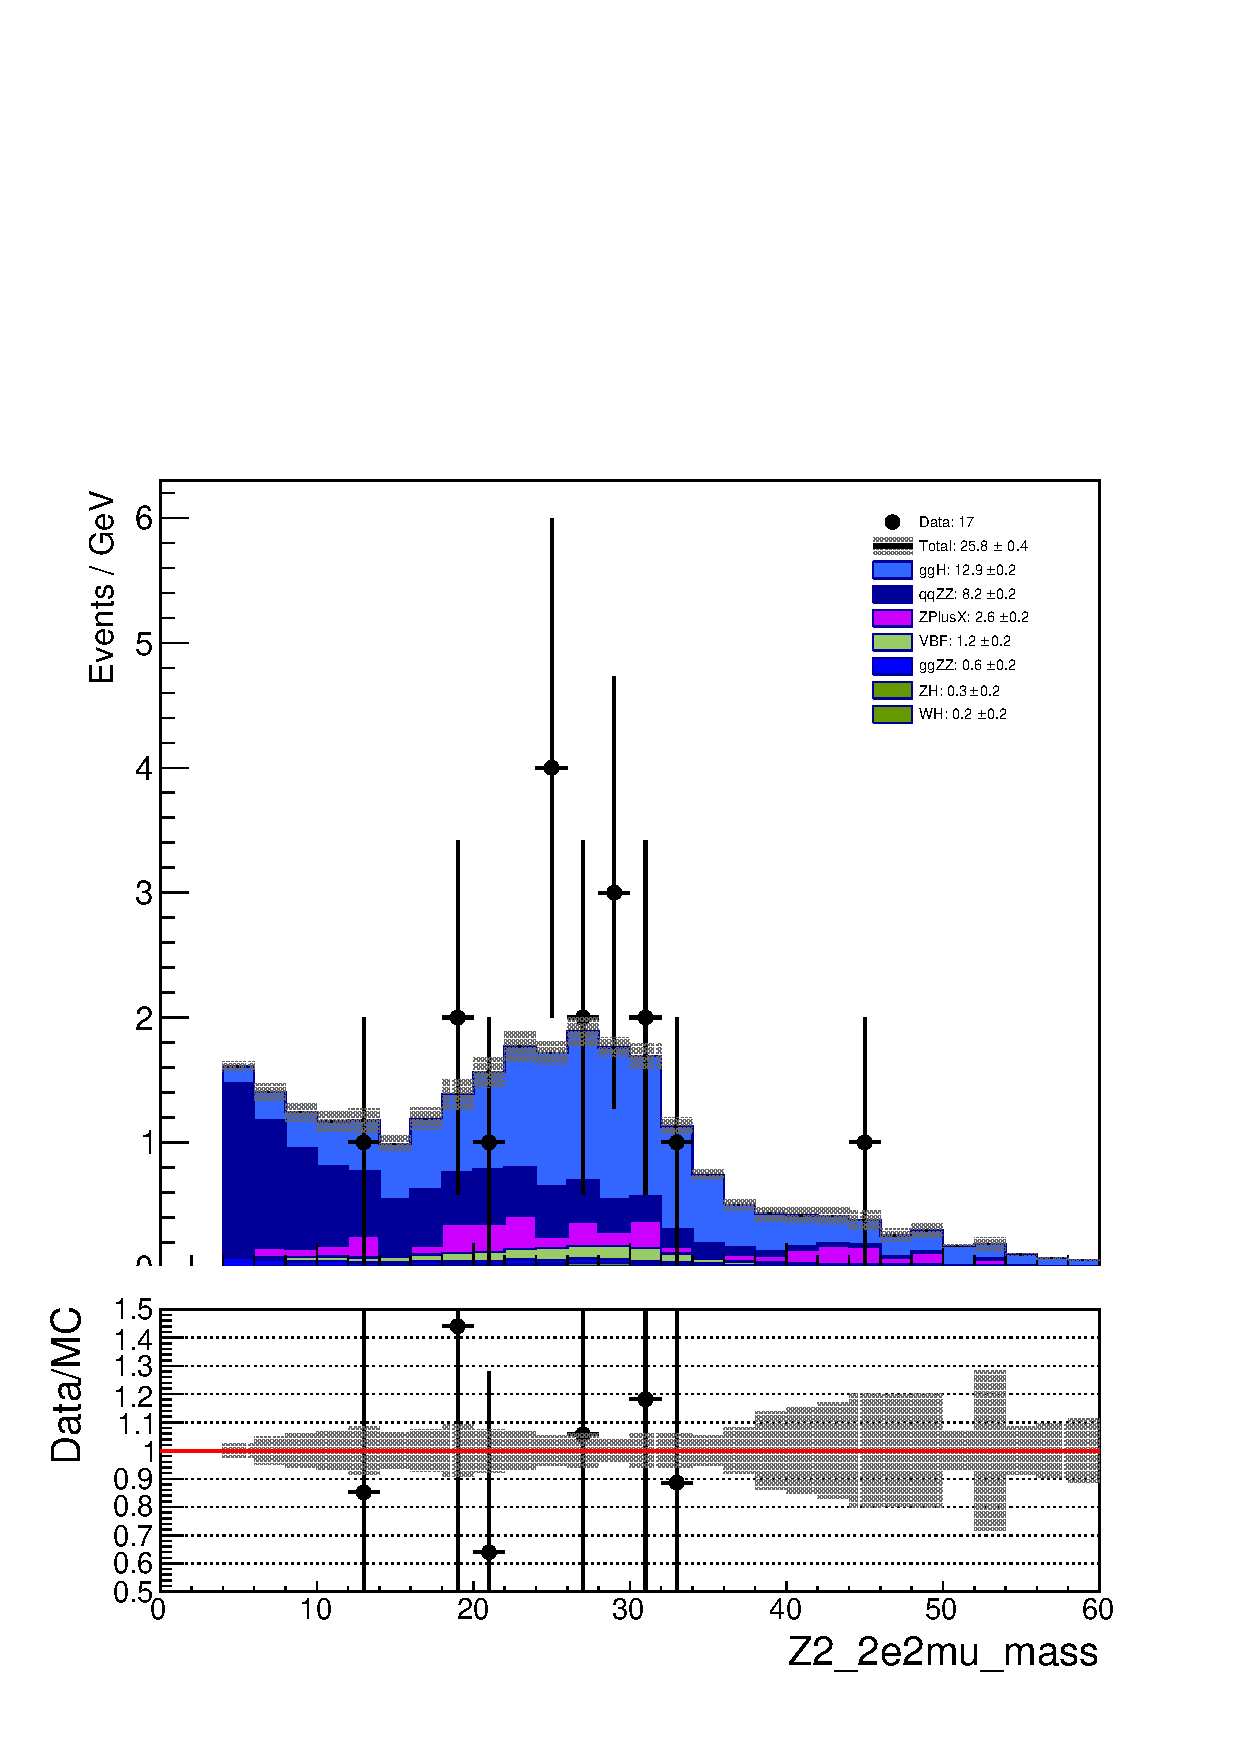
\includegraphics[width=0.45\textwidth]{Figures/Results/Distributions/DarkPhotonSR17/Z2_2e2mu_mass}}
{ 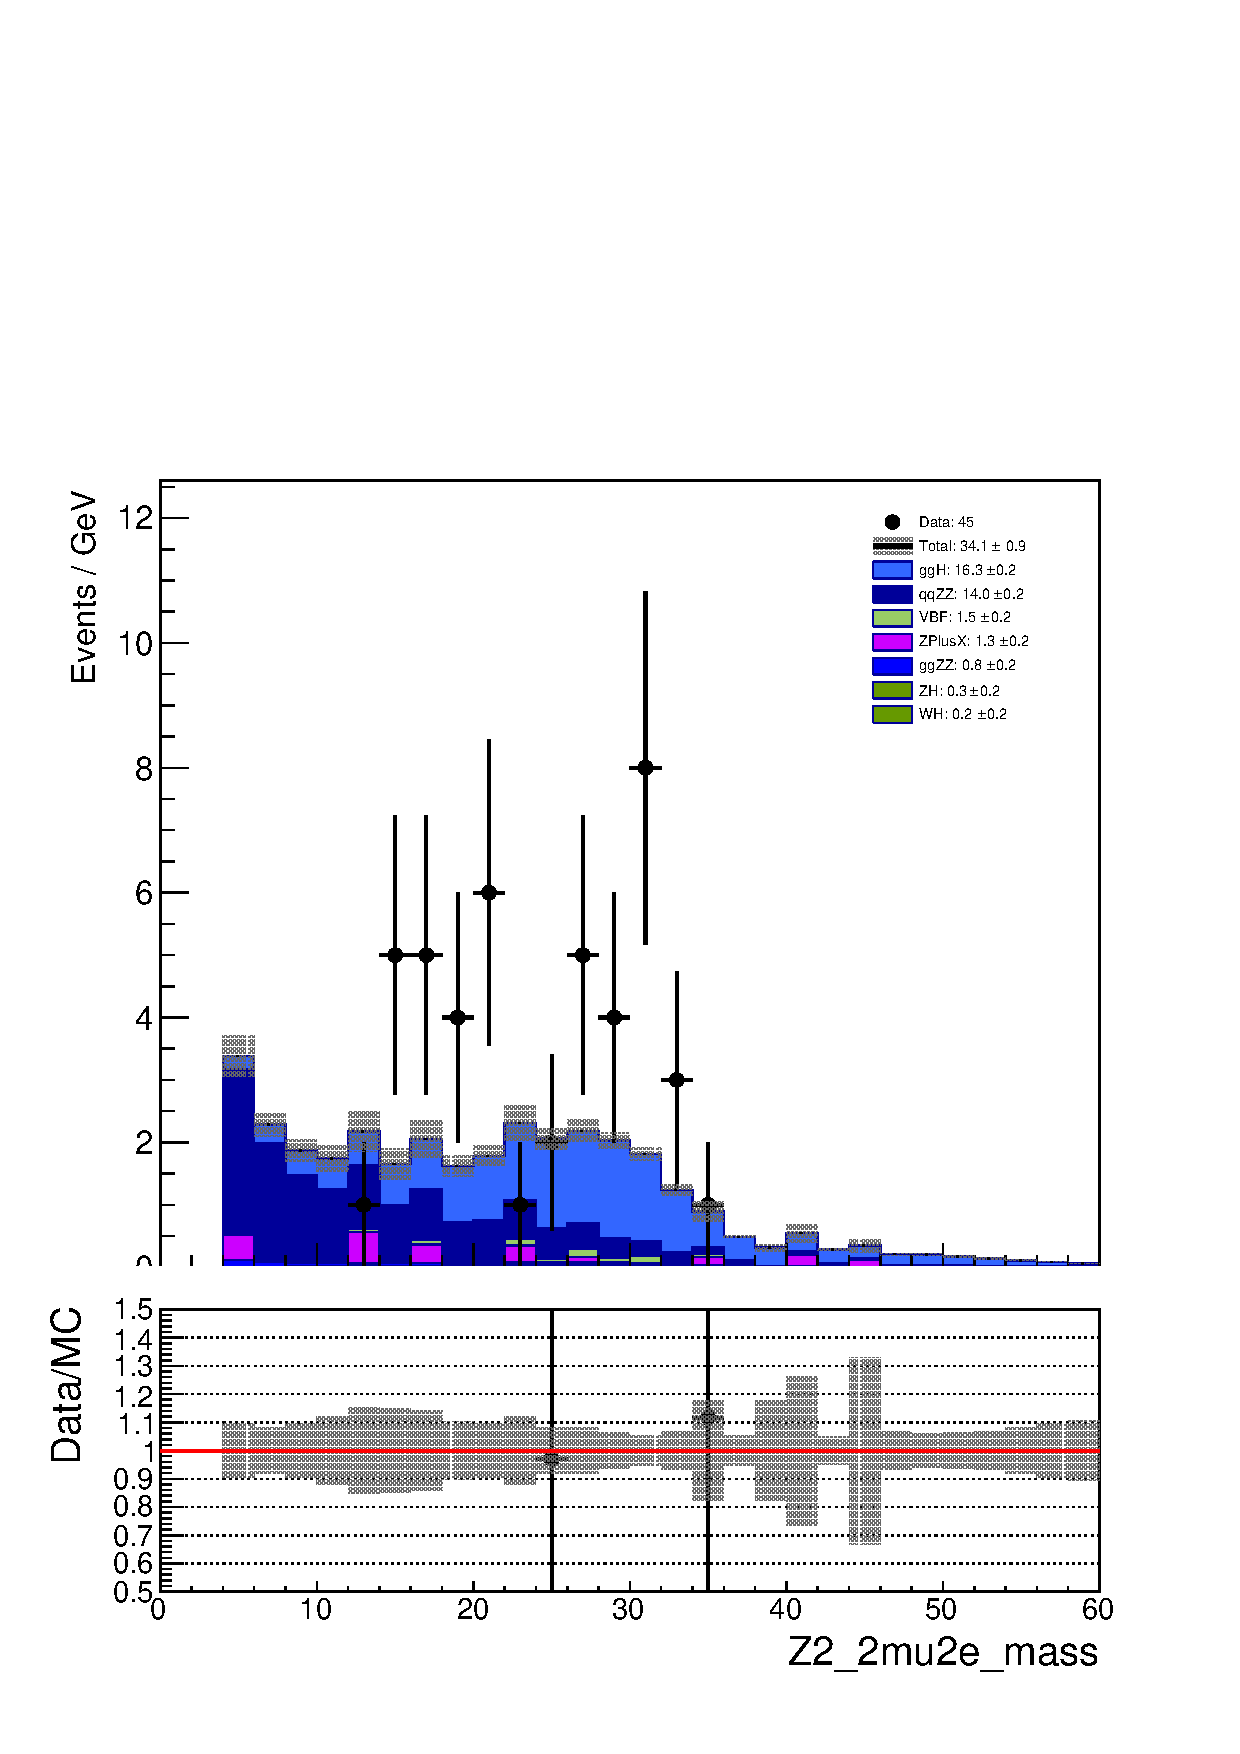
\includegraphics[width=0.45\textwidth]{Figures/Results/Distributions/DarkPhotonSR17/Z2_2mu2e_mass}}
\caption{Distributions of the reconstructed \mass{Z2} and a comparison to predicted backgrounds using 2017 dataset. Different \zd signal hypothesis are also shown.
\label{fig:massZ2_17}}
\end{figure}

